%% 
%% Copyright 2019-2024 Elsevier Ltd
%% 
%% This file is part of the 'CAS Bundle'.
%% --------------------------------------
%% 
%% It may be distributed under the conditions of the LaTeX Project Public
%% License, either version 1.3c of this license or (at your option) any
%% later version.  The latest version of this license is in
%%    http://www.latex-project.org/lppl.txt
%% and version 1.3c or later is part of all distributions of LaTeX
%% version 1999/12/01 or later.
%% 
%% The list of all files belonging to the 'CAS Bundle' is
%% given in the file `manifest.txt'.
%% 
%% Template article for cas-sc documentclass for 
%% double column output.

\documentclass[a4paper,fleqn]{cas-sc}

% If the frontmatter runs over more than one page
% use the longmktitle option.

%\documentclass[a4paper,fleqn,longmktitle]{cas-sc}

%\usepackage[numbers]{natbib}
%\usepackage[authoryear]{natbib}
\usepackage[authoryear]{natbib}
\usepackage{amssymb}
%% The amsmath package provides various useful equation environments.
\usepackage{amsmath}
\usepackage[T1]{fontenc}
\usepackage[utf8]{inputenc}
\usepackage{graphicx}
\usepackage{amssymb}
\graphicspath{ {./images/} }
\usepackage{booktabs}
\usepackage{array}
\usepackage{tabularx}
\usepackage{aligned-overset}
\usepackage{bm}
\usepackage{float}
\usepackage{hyperref}
\usepackage{xcolor}
\usepackage{comment}
\usepackage{longtable}
\usepackage{pdflscape}
\usepackage{tikz}
\usetikzlibrary{shapes.geometric, arrows.meta, positioning, calc, fit, backgrounds}
%%%Author macros
\def\tsc#1{\csdef{#1}{\textsc{\lowercase{#1}}\xspace}}
\tsc{WGM}
\tsc{QE}
%%%

% Avoid spaces after figures 
\setlength{\floatsep}{12pt plus 2pt minus 2pt}
\setlength{\textfloatsep}{12pt plus 2pt minus 2pt}

% A generated table, typeset at the full text width. Every table in latex/ is a tabularx or a tabular* that
% already fills \textwidth, so no template has to box or scale one; this hook stays so that a journal needing
% something of its own can redefine it in one place.
\newcommand{\projtable}[1]{\input{#1}}

% One declaration: the statement is shared, the heading belongs to the layout. The declarations are
% listed in sections/manuscript_declarations.tex and this is the only place a layout decides how they
% are presented.
\newcommand{\projdeclaration}[2]{\section*{#1}\input{#2}}

% The front matter as data: title, authors, their e-mail, ORCID and contributions, and the one affiliation.
% No journal's syntax appears here, because every class asks for the same facts in a different shape: one wants
% a single name per author with the address as key=value pairs, another wants the given and family names split
% into separate commands and the address broken into fields of its own, and the reading copy wants one
% \and-separated line. So this file states each fact once and a template renders it, exactly as the abstract and
% the keywords already work. Supporting one more journal means writing the renderers below in the new
% template, and changing nothing here.
%
% A template must define, before it uses \projauthorlist:
%   \projauthor{initials}{given}{family}{email}{orcid}{CRediT roles}      one non-corresponding author
%   \projauthorcorr{...}                                                 same six, for the corresponding author
% ORCID may be empty, so a renderer that prints it guards the field with \projifhasorcid.

\newcommand{\projtitle}{Leakage-Free Benchmarking of Classical Machine Learning and Graph Neural Networks for Low-Data TgDHFR Bioactivity Prediction}
\newcommand{\projshorttitle}{Leakage-Free Benchmarking of Classical ML and Graph Neural Networks}
\newcommand{\projrunningauthors}{Vinajera-Zamora et al., 2026}

\newcommand{\projaffildiv}{Instituto Universitario de Investigaci\'on y Desarrollo Tecnol\'ogico}
\newcommand{\projaffilorg}{Universidad Tecnol\'ogica Metropolitana}
\newcommand{\projaffilstreet}{Ignacio Valdivieso 2409}
\newcommand{\projaffilcity}{Santiago}
\newcommand{\projaffilstate}{Regi\'on Metropolitana}
\newcommand{\projaffilpostcode}{97279}
\newcommand{\projaffilcountry}{Chile}

% Not every author has an ORCID on file, and a renderer that prints the field unconditionally would emit an empty
% link for the ones who do not. This runs its second argument only when the first is a non-empty ORCID.
\newcommand{\projifhasorcid}[2]{\def\projorcidarg{#1}\ifx\projorcidarg\empty\else#2\fi}

% The authors in the order they appear on the paper. The corresponding author is marked by which macro the line
% calls, not by a flag, so no layout has to decide what "corresponding" looks like in its own notation.
% The roles are the CRediT taxonomy's own terms: they go into the author block of a class that has one, and into
% the contributions declaration, which is rendered from this same list.
\newcommand{\projauthorlist}{%
	\projauthorcorr{A.V.-Z.}{Andrey}{Vinajera-Zamora}{avinajera@utem.cl}{0000-0002-4922-457X}%
		{Conceptualization, Methodology, Formal analysis, Software, Validation, Investigation,
		 Writing -- original draft, Visualization}%
	\projauthor{J.C.-G.}{Juan}{Castillo-Garit}{j.castillo@utem.cl}{0000-0003-0896-9484}%
		{Methodology, Validation, Writing -- review \& editing, Supervision}%
	\projauthor{S.M.-S.}{Samuel}{Montejo-S\'anchez}{smontejo@utem.cl}{0000-0003-1622-3180}%
		{Validation, Writing -- review \& editing, Supervision}%
	\projauthor{R.A.-C.}{Raul}{Arias-Carrasco}{raul.arias@utem.cl}{0000-0003-1698-9282}%
		{Validation, Supervision, Writing -- review \& editing, Visualization}%
}

% Every macro file the pipeline generates, in one place, so that a template or the supplement needs a single
% \input instead of sixteen. This file is written by hand, which is why it lives here and not in latex/:
% everything in that directory is a build product. Step 11 follows this chain, so a document that reads this
% file is verified like the others. A new step that writes macros adds its line here and nowhere else.
% =====================================================
% Nested CV Benchmark Variables (Auto-generated)
% =====================================================

\newcommand{\NCompounds}{859}
\newcommand{\OuterKFolds}{5}
\newcommand{\OuterRepeats}{5}
\newcommand{\TotalOuterFolds}{25}
\newcommand{\InnerKFolds}{5}
\newcommand{\MaxComboSize}{3}

\newcommand{\PaperBaselineRTwo}{0.75}
\newcommand{\PaperSelectedRTwo}{0.82}
\newcommand{\PaperFinalRTwo}{0.85}

\newcommand{\RdkitTwoDThreeDFpRTwoMean}{0.774}
\newcommand{\RdkitTwoDThreeDFpRTwoStd}{0.041}
\newcommand{\RdkitTwoDThreeDFpNFolds}{25}
\newcommand{\RdkitTwoDThreeDFpBestArchitecture}{ET+LGBM+SVM}
\newcommand{\RdkitTwoDThreeDFpBestArchitectureSafe}{ETLGBMSVM}
\newcommand{\RdkitTwoDThreeDFpStability}{60.0}
\newcommand{\RdkitTwoDThreeDFpMaeMean}{0.428}
\newcommand{\RdkitTwoDThreeDFpNFeaturesTotal}{2275}
\newcommand{\RdkitTwoDThreeDFpNFeaturesSelectedMean}{1312.7}
\newcommand{\SelRdkitTwoDThreeDFpRFPct}{8}
\newcommand{\SelRdkitTwoDThreeDFpETPct}{100}
\newcommand{\SelRdkitTwoDThreeDFpLGBMPct}{60}
\newcommand{\SelRdkitTwoDThreeDFpXGBPct}{4}
\newcommand{\SelRdkitTwoDThreeDFpSVMPct}{100}
\newcommand{\SelRdkitTwoDThreeDFpkNNPct}{8}
\newcommand{\SelRdkitTwoDThreeDFpSizeOnePct}{0}
\newcommand{\SelRdkitTwoDThreeDFpSizeTwoPct}{20}
\newcommand{\SelRdkitTwoDThreeDFpSizeThreePct}{80}
\newcommand{\SelRdkitTwoDThreeDFpNArchitectures}{5}
\newcommand{\SelRdkitTwoDThreeDFpTopCount}{15}
\newcommand{\SelRdkitTwoDThreeDFpSecond}{ET+SVM}
\newcommand{\SelRdkitTwoDThreeDFpSecondCount}{5}
\newcommand{\SelRdkitTwoDThreeDFpOthersMaxCount}{2}
\newcommand{\SelRdkitTwoDThreeDFpNOthers}{3}
\newcommand{\RdkitTwoDFpRTwoMean}{0.774}
\newcommand{\RdkitTwoDFpRTwoStd}{0.043}
\newcommand{\RdkitTwoDFpNFolds}{25}
\newcommand{\RdkitTwoDFpBestArchitecture}{ET+LGBM+SVM}
\newcommand{\RdkitTwoDFpBestArchitectureSafe}{ETLGBMSVM}
\newcommand{\RdkitTwoDFpStability}{32.0}
\newcommand{\RdkitTwoDFpMaeMean}{0.428}
\newcommand{\RdkitTwoDFpNFeaturesTotal}{2265}
\newcommand{\RdkitTwoDFpNFeaturesSelectedMean}{1320.6}
\newcommand{\SelRdkitTwoDFpRFPct}{20}
\newcommand{\SelRdkitTwoDFpETPct}{100}
\newcommand{\SelRdkitTwoDFpLGBMPct}{36}
\newcommand{\SelRdkitTwoDFpXGBPct}{16}
\newcommand{\SelRdkitTwoDFpSVMPct}{96}
\newcommand{\SelRdkitTwoDFpkNNPct}{8}
\newcommand{\SelRdkitTwoDFpSizeOnePct}{0}
\newcommand{\SelRdkitTwoDFpSizeTwoPct}{24}
\newcommand{\SelRdkitTwoDFpSizeThreePct}{76}
\newcommand{\SelRdkitTwoDFpNArchitectures}{6}
\newcommand{\SelRdkitTwoDFpTopCount}{8}
\newcommand{\SelRdkitTwoDFpSecond}{ET+SVM}
\newcommand{\SelRdkitTwoDFpSecondCount}{6}
\newcommand{\SelRdkitTwoDFpOthersMaxCount}{4}
\newcommand{\SelRdkitTwoDFpNOthers}{4}
\newcommand{\MorganRTwoMean}{0.769}
\newcommand{\MorganRTwoStd}{0.041}
\newcommand{\MorganNFolds}{25}
\newcommand{\MorganBestArchitecture}{RF+XGB+SVM}
\newcommand{\MorganBestArchitectureSafe}{RFXGBSVM}
\newcommand{\MorganStability}{76.0}
\newcommand{\MorganMaeMean}{0.434}
\newcommand{\MorganNFeaturesTotal}{2048}
\newcommand{\MorganNFeaturesSelectedMean}{2048.0}
\newcommand{\SelMorganRFPct}{84}
\newcommand{\SelMorganETPct}{4}
\newcommand{\SelMorganLGBMPct}{4}
\newcommand{\SelMorganXGBPct}{92}
\newcommand{\SelMorganSVMPct}{100}
\newcommand{\SelMorgankNNPct}{12}
\newcommand{\SelMorganSizeOnePct}{0}
\newcommand{\SelMorganSizeTwoPct}{4}
\newcommand{\SelMorganSizeThreePct}{96}
\newcommand{\SelMorganNArchitectures}{5}
\newcommand{\SelMorganTopCount}{19}
\newcommand{\SelMorganSecond}{XGB+SVM+kNN}
\newcommand{\SelMorganSecondCount}{3}
\newcommand{\SelMorganOthersMaxCount}{1}
\newcommand{\SelMorganNOthers}{3}
\newcommand{\RdkitTwoDRTwoMean}{0.728}
\newcommand{\RdkitTwoDRTwoStd}{0.048}
\newcommand{\RdkitTwoDNFolds}{25}
\newcommand{\RdkitTwoDBestArchitecture}{ET+LGBM+SVM}
\newcommand{\RdkitTwoDBestArchitectureSafe}{ETLGBMSVM}
\newcommand{\RdkitTwoDStability}{52.0}
\newcommand{\RdkitTwoDMaeMean}{0.468}
\newcommand{\RdkitTwoDNFeaturesTotal}{217}
\newcommand{\RdkitTwoDNFeaturesSelectedMean}{184.8}
\newcommand{\SelRdkitTwoDRFPct}{28}
\newcommand{\SelRdkitTwoDETPct}{100}
\newcommand{\SelRdkitTwoDLGBMPct}{56}
\newcommand{\SelRdkitTwoDXGBPct}{0}
\newcommand{\SelRdkitTwoDSVMPct}{92}
\newcommand{\SelRdkitTwoDkNNPct}{0}
\newcommand{\SelRdkitTwoDSizeOnePct}{4}
\newcommand{\SelRdkitTwoDSizeTwoPct}{16}
\newcommand{\SelRdkitTwoDSizeThreePct}{80}
\newcommand{\SelRdkitTwoDNArchitectures}{5}
\newcommand{\SelRdkitTwoDTopCount}{13}
\newcommand{\SelRdkitTwoDSecond}{RF+ET+SVM}
\newcommand{\SelRdkitTwoDSecondCount}{7}
\newcommand{\SelRdkitTwoDOthersMaxCount}{3}
\newcommand{\SelRdkitTwoDNOthers}{3}

\newcommand{\NClippedPredictions}{0}
\newcommand{\NArchitectureCombos}{41}
\newcommand{\NInnerFitsPerOuterFold}{205}
\newcommand{\MorganNCellsMissing}{0}
\newcommand{\MorganNThreeDFailed}{0}
\newcommand{\MorganFeaturizationSec}{0.4}
\newcommand{\RdkitTwoDNCellsMissing}{0}
\newcommand{\RdkitTwoDNThreeDFailed}{0}
\newcommand{\RdkitTwoDFeaturizationSec}{3.8}
\newcommand{\RdkitTwoDFpNCellsMissing}{0}
\newcommand{\RdkitTwoDFpNThreeDFailed}{0}
\newcommand{\RdkitTwoDFpFeaturizationSec}{1.8}
\newcommand{\RdkitTwoDThreeDFpNCellsMissing}{0}
\newcommand{\RdkitTwoDThreeDFpNThreeDFailed}{0}
\newcommand{\RdkitTwoDThreeDFpFeaturizationSec}{6.9}

\newcommand{\PValueMorganVsPaperBaseline}{0.3971}
\newcommand{\TStatMorganVsPaperBaseline}{0.862}
\newcommand{\SigDiffMorganVsPaperBaseline}{false}
\newcommand{\PValueMorganVsPaperSelected}{0.0280}
\newcommand{\TStatMorganVsPaperSelected}{-2.339}
\newcommand{\SigDiffMorganVsPaperSelected}{true}
\newcommand{\PValueMorganVsPaperFinal}{0.0011}
\newcommand{\TStatMorganVsPaperFinal}{-3.712}
\newcommand{\SigDiffMorganVsPaperFinal}{true}
\newcommand{\PValueRdkitTwoDVsPaperBaseline}{0.4088}
\newcommand{\TStatRdkitTwoDVsPaperBaseline}{-0.841}
\newcommand{\SigDiffRdkitTwoDVsPaperBaseline}{false}
\newcommand{\PValueRdkitTwoDVsPaperSelected}{0.0017}
\newcommand{\TStatRdkitTwoDVsPaperSelected}{-3.527}
\newcommand{\SigDiffRdkitTwoDVsPaperSelected}{true}
\newcommand{\PValueRdkitTwoDVsPaperFinal}{0.0001}
\newcommand{\TStatRdkitTwoDVsPaperFinal}{-4.679}
\newcommand{\SigDiffRdkitTwoDVsPaperFinal}{true}
\newcommand{\PValueRdkitTwoDFpVsPaperBaseline}{0.3187}
\newcommand{\TStatRdkitTwoDFpVsPaperBaseline}{1.018}
\newcommand{\SigDiffRdkitTwoDFpVsPaperBaseline}{false}
\newcommand{\PValueRdkitTwoDFpVsPaperSelected}{0.0553}
\newcommand{\TStatRdkitTwoDFpVsPaperSelected}{-2.014}
\newcommand{\SigDiffRdkitTwoDFpVsPaperSelected}{false}
\newcommand{\PValueRdkitTwoDFpVsPaperFinal}{0.0029}
\newcommand{\TStatRdkitTwoDFpVsPaperFinal}{-3.314}
\newcommand{\SigDiffRdkitTwoDFpVsPaperFinal}{true}
\newcommand{\PValueRdkitTwoDThreeDFpVsPaperBaseline}{0.2862}
\newcommand{\TStatRdkitTwoDThreeDFpVsPaperBaseline}{1.091}
\newcommand{\SigDiffRdkitTwoDThreeDFpVsPaperBaseline}{false}
\newcommand{\PValueRdkitTwoDThreeDFpVsPaperSelected}{0.0486}
\newcommand{\TStatRdkitTwoDThreeDFpVsPaperSelected}{-2.078}
\newcommand{\SigDiffRdkitTwoDThreeDFpVsPaperSelected}{true}
\newcommand{\PValueRdkitTwoDThreeDFpVsPaperFinal}{0.0022}
\newcommand{\TStatRdkitTwoDThreeDFpVsPaperFinal}{-3.436}
\newcommand{\SigDiffRdkitTwoDThreeDFpVsPaperFinal}{true}

\newcommand{\TopModeOne}{RdkitTwoDThreeDFp}
\newcommand{\TopModeTwo}{RdkitTwoDFp}
\newcommand{\PairedTTestStat}{0.224}
\newcommand{\PairedTTestP}{0.8243}

\newcommand{\WinnerMode}{RdkitTwoDThreeDFp}
\newcommand{\WinnerRTwoMean}{0.774}
\newcommand{\WinnerRTwoStd}{0.041}
\newcommand{\InnerRepeats}{5}
\newcommand{\MorganPooledRTwoMean}{0.771}
\newcommand{\MorganPooledRTwoMin}{0.761}
\newcommand{\MorganPooledRTwoMax}{0.779}
\newcommand{\MorganPooledMaeMean}{0.434}
\newcommand{\MorganPooledMaeMin}{0.429}
\newcommand{\MorganPooledMaeMax}{0.441}
\newcommand{\RdkitTwoDPooledRTwoMean}{0.731}
\newcommand{\RdkitTwoDPooledRTwoMin}{0.717}
\newcommand{\RdkitTwoDPooledRTwoMax}{0.743}
\newcommand{\RdkitTwoDPooledMaeMean}{0.468}
\newcommand{\RdkitTwoDPooledMaeMin}{0.456}
\newcommand{\RdkitTwoDPooledMaeMax}{0.483}
\newcommand{\RdkitTwoDThreeDFpPooledRTwoMean}{0.776}
\newcommand{\RdkitTwoDThreeDFpPooledRTwoMin}{0.767}
\newcommand{\RdkitTwoDThreeDFpPooledRTwoMax}{0.784}
\newcommand{\RdkitTwoDThreeDFpPooledMaeMean}{0.428}
\newcommand{\RdkitTwoDThreeDFpPooledMaeMin}{0.420}
\newcommand{\RdkitTwoDThreeDFpPooledMaeMax}{0.438}
\newcommand{\RdkitTwoDFpPooledRTwoMean}{0.776}
\newcommand{\RdkitTwoDFpPooledRTwoMin}{0.769}
\newcommand{\RdkitTwoDFpPooledRTwoMax}{0.784}
\newcommand{\RdkitTwoDFpPooledMaeMean}{0.428}
\newcommand{\RdkitTwoDFpPooledMaeMin}{0.420}
\newcommand{\RdkitTwoDFpPooledMaeMax}{0.435}

% =====================================================
% Variables auto-generated by 04_augmentation_training.py
% Includes rigorous bootstrap CIs and non-parametric p-values
% =====================================================

\newcommand{\ExpNDev}{730}
\newcommand{\ExpNTest}{129}

% --- Experiment A: Baseline Stacking (No Feat Sel, No Aug) ---
\newcommand{\ExpARTwoMean}{0.7341}
\newcommand{\ExpAMae}{0.4378}
\newcommand{\ExpARTwoCILow}{0.6278}
\newcommand{\ExpARTwoCIHigh}{0.8176}

% --- Experiment B: Permutation Importance Selection ---
\newcommand{\ExpBRTwoMean}{0.7409}
\newcommand{\ExpBMae}{0.4376}
\newcommand{\ExpBRTwoCILow}{0.6394}
\newcommand{\ExpBRTwoCIHigh}{0.8218}
\newcommand{\ExpBNFeaturesTotal}{2048}
\newcommand{\ExpBNFeaturesSelected}{765}

% --- Experiment C: Feature Selection + Gaussian Augmentation ---
\newcommand{\ExpCRTwoMean}{0.7233}
\newcommand{\ExpCMae}{0.4485}
\newcommand{\ExpCRTwoCILow}{0.6119}
\newcommand{\ExpCRTwoCIHigh}{0.8115}
\newcommand{\ExpCAugFactor}{3}
\newcommand{\ExpCAugSizeTrain}{2190}
\newcommand{\ExpCNoiseLevels}{0.01, 0.001}

% --- Diagnostic: Experiments B/C with selection on the test set (leaky, original-study protocol) ---
\newcommand{\ExpBleakyRTwoMean}{0.8303}
\newcommand{\ExpBleakyMae}{0.3507}
\newcommand{\ExpBleakyRTwoCILow}{0.7521}
\newcommand{\ExpBleakyRTwoCIHigh}{0.8900}
\newcommand{\ExpBleakyNFeaturesSelected}{463}
\newcommand{\ExpCleakyRTwoMean}{0.8315}
\newcommand{\ExpCleakyMae}{0.3563}
\newcommand{\ExpCleakyRTwoCILow}{0.7555}
\newcommand{\ExpCleakyRTwoCIHigh}{0.8881}
\newcommand{\ExpCleakyNFeaturesSelected}{463}
\newcommand{\ExpLeakyMaskJaccard}{0.3319}

% --- Reference Benchmarks ---
\providecommand{\PaperBaselineRTwo}{0.75}
\providecommand{\PaperSelectedRTwo}{0.82}
\providecommand{\PaperFinalRTwo}{0.85}

% --- Rigorous Statistical Evaluations vs Benchmarks ---
\newcommand{\ExpAVsPaperBaselineInCI}{true}
\newcommand{\ExpAVsPaperBaselinePBoot}{0.7230}
\newcommand{\ExpAVsPaperBaselineSig}{false}
\newcommand{\ExpAVsPaperSelectedInCI}{false}
\newcommand{\ExpAVsPaperSelectedPBoot}{0.0470}
\newcommand{\ExpAVsPaperSelectedSig}{true}
\newcommand{\ExpAVsPaperFinalInCI}{false}
\newcommand{\ExpAVsPaperFinalPBoot}{0.0050}
\newcommand{\ExpAVsPaperFinalSig}{true}
\newcommand{\ExpBVsPaperBaselineInCI}{true}
\newcommand{\ExpBVsPaperBaselinePBoot}{0.8260}
\newcommand{\ExpBVsPaperBaselineSig}{false}
\newcommand{\ExpBVsPaperSelectedInCI}{true}
\newcommand{\ExpBVsPaperSelectedPBoot}{0.0610}
\newcommand{\ExpBVsPaperSelectedSig}{false}
\newcommand{\ExpBVsPaperFinalInCI}{false}
\newcommand{\ExpBVsPaperFinalPBoot}{0.0060}
\newcommand{\ExpBVsPaperFinalSig}{true}
\newcommand{\ExpCVsPaperBaselineInCI}{true}
\newcommand{\ExpCVsPaperBaselinePBoot}{0.5930}
\newcommand{\ExpCVsPaperBaselineSig}{false}
\newcommand{\ExpCVsPaperSelectedInCI}{false}
\newcommand{\ExpCVsPaperSelectedPBoot}{0.0280}
\newcommand{\ExpCVsPaperSelectedSig}{true}
\newcommand{\ExpCVsPaperFinalInCI}{false}
\newcommand{\ExpCVsPaperFinalPBoot}{0.0040}
\newcommand{\ExpCVsPaperFinalSig}{true}
\newcommand{\ExpBleakyVsPaperBaselineInCI}{false}
\newcommand{\ExpBleakyVsPaperBaselinePBoot}{0.0440}
\newcommand{\ExpBleakyVsPaperBaselineSig}{true}
\newcommand{\ExpBleakyVsPaperSelectedInCI}{true}
\newcommand{\ExpBleakyVsPaperSelectedPBoot}{0.7580}
\newcommand{\ExpBleakyVsPaperSelectedSig}{false}
\newcommand{\ExpBleakyVsPaperFinalInCI}{true}
\newcommand{\ExpBleakyVsPaperFinalPBoot}{0.5450}
\newcommand{\ExpBleakyVsPaperFinalSig}{false}
\newcommand{\ExpCleakyVsPaperBaselineInCI}{false}
\newcommand{\ExpCleakyVsPaperBaselinePBoot}{0.0340}
\newcommand{\ExpCleakyVsPaperBaselineSig}{true}
\newcommand{\ExpCleakyVsPaperSelectedInCI}{true}
\newcommand{\ExpCleakyVsPaperSelectedPBoot}{0.7330}
\newcommand{\ExpCleakyVsPaperSelectedSig}{false}
\newcommand{\ExpCleakyVsPaperFinalInCI}{true}
\newcommand{\ExpCleakyVsPaperFinalPBoot}{0.5450}
\newcommand{\ExpCleakyVsPaperFinalSig}{false}

% --- Paired bootstrap R2 differences (same resampled test indices) ---
\newcommand{\ExpCvsADeltaRTwo}{-0.0108}
\newcommand{\ExpCvsADeltaCILow}{-0.0431}
\newcommand{\ExpCvsADeltaCIHigh}{+0.0152}
\newcommand{\ExpCvsADeltaPBoot}{0.4300}
\newcommand{\ExpBvsADeltaRTwo}{+0.0068}
\newcommand{\ExpBvsADeltaCILow}{-0.0223}
\newcommand{\ExpBvsADeltaCIHigh}{+0.0326}
\newcommand{\ExpBvsADeltaPBoot}{0.6140}
\newcommand{\ExpCvsBDeltaRTwo}{-0.0176}
\newcommand{\ExpCvsBDeltaCILow}{-0.0360}
\newcommand{\ExpCvsBDeltaCIHigh}{-0.0018}
\newcommand{\ExpCvsBDeltaPBoot}{0.0250}
\newcommand{\ExpBleakyvsADeltaRTwo}{+0.0962}
\newcommand{\ExpBleakyvsADeltaCILow}{+0.0548}
\newcommand{\ExpBleakyvsADeltaCIHigh}{+0.1471}
\newcommand{\ExpBleakyvsADeltaPBoot}{0.0000}
\newcommand{\ExpBleakyvsBDeltaRTwo}{+0.0894}
\newcommand{\ExpBleakyvsBDeltaCILow}{+0.0458}
\newcommand{\ExpBleakyvsBDeltaCIHigh}{+0.1424}
\newcommand{\ExpBleakyvsBDeltaPBoot}{0.0000}
\newcommand{\ExpCleakyvsCDeltaRTwo}{+0.1082}
\newcommand{\ExpCleakyvsCDeltaCILow}{+0.0615}
\newcommand{\ExpCleakyvsCDeltaCIHigh}{+0.1676}
\newcommand{\ExpCleakyvsCDeltaPBoot}{0.0000}

% Auto-generated by 07_molecular_docking.py
% Include with: \input{docking_variables.tex}

\newcommand{\DockNTotal}{17}
\newcommand{\DockNValidated}{5}
\newcommand{\DockNDiscordant}{1}
\newcommand{\DockExhaustiveness}{32}
\newcommand{\DockBoxSize}{20.0}
\newcommand{\DockCenterX}{3.689}
\newcommand{\DockCenterY}{39.992}
\newcommand{\DockCenterZ}{-62.818}
\newcommand{\DockMLActiveThresh}{6.5}
\newcommand{\DockActiveThresh}{-8.0}
\newcommand{\DockMLInactiveThresh}{6.0}
\newcommand{\DockInactiveThresh}{-7.5}
\newcommand{\DockNPoses}{3}
\newcommand{\DockSpearmanRho}{-0.422}
\newcommand{\DockSpearmanP}{0.0911}
\newcommand{\DockNNegative}{0}
\newcommand{\DockNFalseNegative}{2}
\newcommand{\DockNNeutral}{9}
\newcommand{\DockNValidatedUnique}{4}
\newcommand{\DockBestCandidate}{TrimetrexateGlucuron}
\newcommand{\DockBestMLpIC}{7.4136}
\newcommand{\DockBestDockScore}{-8.76}
\newcommand{\DockRawBestDockScore}{-9.43}
\newcommand{\BisacodylMLpIC}{4.9568}
\newcommand{\BisacodylDockScore}{-8.82}
\newcommand{\PyrimethamineMLpIC}{6.5315}
\newcommand{\PyrimethamineDockScore}{-7.62}
\newcommand{\FolicAcidMLpIC}{6.3026}
\newcommand{\FolicAcidDockScore}{-9.43}
\newcommand{\MethotrexateMLpIC}{7.4421}
\newcommand{\MethotrexateDockScore}{-8.66}
\newcommand{\TriamtereneMLpIC}{6.9270}
\newcommand{\TriamtereneDockScore}{-8.07}
\newcommand{\PralatrexateMLpIC}{7.1170}
\newcommand{\PralatrexateDockScore}{-8.68}
\newcommand{\TrimetrexateMLpIC}{7.4136}
\newcommand{\TrimetrexateDockScore}{-8.76}
\newcommand{\TrimethoprimMLpIC}{5.7171}
\newcommand{\TrimethoprimDockScore}{-7.56}

% Auto-generated by 05_virtual_screening.py
\newcommand{\ScreenNLibrary}{3378}
\newcommand{\ScreenNStructural}{3056}
\newcommand{\ScreenNDomain}{14}
\newcommand{\ScreenNCandidates}{17}
\newcommand{\ScreenNTopML}{10}
\newcommand{\ScreenNReference}{7}
\newcommand{\ScreenNTrainMols}{859}
\newcommand{\ScreenMaskBits}{747}
\newcommand{\ScreenMaxMW}{1000}
\newcommand{\ScreenADNeighbors}{5}
\newcommand{\ScreenADZ}{0.5}
\newcommand{\ScreenADMinSimilarity}{0.638}
\newcommand{\ScreenConformalHalfWidth}{0.99}
\newcommand{\ScreenConformalCoverage}{90}
\newcommand{\ScreenConformalNCal}{129}
\newcommand{\ScreenADSensitivityMin}{13}
\newcommand{\ScreenADSensitivityMax}{32}
\newcommand{\ScreenADTrainMedian}{0.70}
\newcommand{\ScreenADFdaMedian}{0.17}
\newcommand{\ScreenADFdaLow}{0.11}
\newcommand{\ScreenADFdaHigh}{0.26}
\newcommand{\ScreenADFdaMax}{0.79}
\newcommand{\ScreenNCandidatesInDomain}{6}
\newcommand{\ScreenNCandidatesInTrain}{7}
\newcommand{\ScreenNCandidatesInDomainNovel}{0}
\newcommand{\ScreenADCandidatesMedian}{0.55}
\newcommand{\ScreenTrainMaxMW}{594}
\newcommand{\ScreenTrainNOutsideElements}{0}
\newcommand{\CandMethotrexatePred}{7.44}
\newcommand{\CandMethotrexateLE}{0.31}
\newcommand{\CandMethotrexateBEI}{16.4}
\newcommand{\CandMethotrexateSim}{0.63}
\newcommand{\CandMethotrexateLower}{6.45}
\newcommand{\CandMethotrexateUpper}{8.44}
\newcommand{\CandTrimetrexatePred}{7.93}
\newcommand{\CandTrimetrexateLE}{0.40}
\newcommand{\CandTrimetrexateBEI}{21.5}
\newcommand{\CandTrimetrexateSim}{0.76}
\newcommand{\CandTrimetrexateLower}{6.94}
\newcommand{\CandTrimetrexateUpper}{8.92}
\newcommand{\CandPralatrexatePred}{7.00}
\newcommand{\CandPralatrexateLE}{0.27}
\newcommand{\CandPralatrexateBEI}{14.7}
\newcommand{\CandPralatrexateSim}{0.49}
\newcommand{\CandPralatrexateLower}{6.01}
\newcommand{\CandPralatrexateUpper}{7.99}
\newcommand{\CandTriamterenePred}{7.01}
\newcommand{\CandTriamtereneLE}{0.51}
\newcommand{\CandTriamtereneBEI}{27.7}
\newcommand{\CandTriamtereneSim}{0.60}
\newcommand{\CandTriamtereneLower}{6.02}
\newcommand{\CandTriamtereneUpper}{8.00}
\newcommand{\CandPyrimethaminePred}{6.57}
\newcommand{\CandPyrimethamineLE}{0.53}
\newcommand{\CandPyrimethamineBEI}{26.4}
\newcommand{\CandPyrimethamineSim}{0.67}
\newcommand{\CandPyrimethamineLower}{5.58}
\newcommand{\CandPyrimethamineUpper}{7.56}
\newcommand{\AntifolateLEMin}{0.27}
\newcommand{\AntifolateLEMax}{0.40}
\newcommand{\ControlPyrimethamineExp}{6.56}
\newcommand{\ControlPyrimethaminePred}{6.57}
\newcommand{\ControlPyrimethamineErr}{0.01}
\newcommand{\ControlTrimethoprimExp}{5.57}
\newcommand{\ControlTrimethoprimPred}{5.67}
\newcommand{\ControlTrimethoprimErr}{0.10}

% Auto-generated by 00_prepare_dataset.py
\newcommand{\DataNRaw}{875}
\newcommand{\DataNOutliers}{2}
\newcommand{\DataNAfterOutliers}{873}
\newcommand{\DataNDuplicatesRemoved}{14}
\newcommand{\DataNMain}{859}
\newcommand{\DataNSensitivity}{861}
\newcommand{\DataNDuplicateGroups}{14}
\newcommand{\DataDuplicateMaxSpread}{0.18}

% Auto-generated by 08_admet_profiling.py
\newcommand{\AdmetNDocked}{17}
\newcommand{\AdmetNLipinski}{14}
\newcommand{\AdmetNHergFlagged}{6}
\newcommand{\AdmetNRemaining}{8}
\newcommand{\AdmetNOral}{6}
\newcommand{\AdmetNParenteral}{2}
\newcommand{\AdmetNHergTrain}{655}
\newcommand{\AdmetNCacoTrain}{910}
\newcommand{\AdmetOverlapHerg}{6}
\newcommand{\AdmetOverlapCaco}{1}
\newcommand{\AdmetHergThresh}{0.5}
\newcommand{\AdmetCacoThresh}{-5.15}
\newcommand{\AdmetLipinskiHBD}{5}
\newcommand{\AdmetLipinskiHBA}{10}
\newcommand{\AdmetLipinskiLogP}{5}
\newcommand{\AdmetNConsensus}{4}
\newcommand{\AdmetNConsensusSurvivors}{3}
\newcommand{\AdmetHergPralatrexate}{0.31}
\newcommand{\AdmetCacoPralatrexate}{-5.41}
\newcommand{\AdmetHergMethotrexate}{0.40}
\newcommand{\AdmetCacoMethotrexate}{-5.87}
\newcommand{\AdmetHergTriamterene}{0.80}
\newcommand{\AdmetCacoTriamterene}{-4.66}
\newcommand{\AdmetHergPyrimethamine}{0.12}
\newcommand{\AdmetCacoPyrimethamine}{-4.42}

% Auto-generated by 09_gnn_baseline.py
\newcommand{\GnnFoldSecMean}{197}
\newcommand{\GnnFoldSecMin}{168}
\newcommand{\GnnFoldSecMax}{210}
\newcommand{\GnnTotalMin}{82}
\newcommand{\GnnSearchFits}{205}
\newcommand{\GnnSearchHoursPerFold}{11}
\newcommand{\GnnSearchDaysTotal}{12}
\newcommand{\ClassicalFoldSecMin}{398}
\newcommand{\ClassicalFoldSecMax}{833}
\newcommand{\ClassicalMorganFoldSec}{614}
\newcommand{\ClassicalMorganTotalHours}{4.3}

\newcommand{\ChemPropDMPNNFoldRTwoMean}{0.7249}
\newcommand{\ChemPropDMPNNFoldMae}{0.4745}
\newcommand{\ChemPropDMPNNFoldRTwoStd}{0.0426}
\newcommand{\ChemPropDMPNNFoldCILow}{0.6775}
\newcommand{\ChemPropDMPNNFoldCIHigh}{0.7722}
\newcommand{\GnnVsMorganDiffRTwo}{-0.0440}
\newcommand{\GnnVsMorganPRTwo}{0.048}
\newcommand{\GnnVsMorganEquivPRTwo}{0.367}
\newcommand{\GnnVsMorganCILowRTwo}{-0.074}
\newcommand{\GnnVsMorganCIHighRTwo}{-0.014}
\newcommand{\GnnVsRdkitTwoDDiffRTwo}{-0.0032}
\newcommand{\GnnVsRdkitTwoDPRTwo}{0.866}
\newcommand{\GnnVsRdkitTwoDEquivPRTwo}{0.010}
\newcommand{\GnnVsRdkitTwoDCILowRTwo}{-0.035}
\newcommand{\GnnVsRdkitTwoDCIHighRTwo}{+0.029}
\newcommand{\GnnVsRdkitTwoDFpDiffRTwo}{-0.0486}
\newcommand{\GnnVsRdkitTwoDFpPRTwo}{0.048}
\newcommand{\GnnVsRdkitTwoDFpEquivPRTwo}{0.471}
\newcommand{\GnnVsRdkitTwoDFpCILowRTwo}{-0.081}
\newcommand{\GnnVsRdkitTwoDFpCIHighRTwo}{-0.017}
\newcommand{\GnnVsRdkitTwoDThreeDFpDiffRTwo}{-0.0492}
\newcommand{\GnnVsRdkitTwoDThreeDFpPRTwo}{0.048}
\newcommand{\GnnVsRdkitTwoDThreeDFpEquivPRTwo}{0.483}
\newcommand{\GnnVsRdkitTwoDThreeDFpCILowRTwo}{-0.080}
\newcommand{\GnnVsRdkitTwoDThreeDFpCIHighRTwo}{-0.018}
\newcommand{\GnnVsMorganDiffMae}{+0.0403}
\newcommand{\GnnVsMorganPMae}{0.031}
\newcommand{\GnnVsMorganEquivPMae}{0.270}
\newcommand{\GnnVsMorganCILowMae}{+0.014}
\newcommand{\GnnVsMorganCIHighMae}{+0.067}
\newcommand{\GnnVsRdkitTwoDDiffMae}{+0.0063}
\newcommand{\GnnVsRdkitTwoDPMae}{0.680}
\newcommand{\GnnVsRdkitTwoDEquivPMae}{0.004}
\newcommand{\GnnVsRdkitTwoDCILowMae}{-0.020}
\newcommand{\GnnVsRdkitTwoDCIHighMae}{+0.032}
\newcommand{\GnnVsRdkitTwoDFpDiffMae}{+0.0468}
\newcommand{\GnnVsRdkitTwoDFpPMae}{0.020}
\newcommand{\GnnVsRdkitTwoDFpEquivPMae}{0.420}
\newcommand{\GnnVsRdkitTwoDFpCILowMae}{+0.020}
\newcommand{\GnnVsRdkitTwoDFpCIHighMae}{+0.074}
\newcommand{\GnnVsRdkitTwoDThreeDFpDiffMae}{+0.0467}
\newcommand{\GnnVsRdkitTwoDThreeDFpPMae}{0.019}
\newcommand{\GnnVsRdkitTwoDThreeDFpEquivPMae}{0.413}
\newcommand{\GnnVsRdkitTwoDThreeDFpCILowMae}{+0.021}
\newcommand{\GnnVsRdkitTwoDThreeDFpCIHighMae}{+0.072}
\newcommand{\GnnVsMinPRTwo}{0.048}
\newcommand{\GnnVsMinPMae}{0.019}

% Auto-generated by 06_redocking_validation.py pipeline
\newcommand{\RedockRMSD}{1.11}
\newcommand{\RedockCentroidDist}{0.35}
\newcommand{\RedockEnergy}{-7.63}
\newcommand{\RedockThreshold}{2.0}
\newcommand{\RedockLigand}{CP6}
\newcommand{\RedockChain}{B}
\newcommand{\RedockCenterX}{3.689}
\newcommand{\RedockCenterY}{39.992}
\newcommand{\RedockCenterZ}{-62.818}
\newcommand{\RedockCenterOffset}{0.001}
\newcommand{\RedockValidated}{true}

% Auto-generated by 02_statistical_tests.py; include with % Auto-generated by 02_statistical_tests.py; include with \input{latex/nadeau_bengio_variables.tex}
\newcommand{\CorrectedTStat}{1.162}
\newcommand{\CorrectedTP}{0.2566}
\newcommand{\NBpRTwoMorganVsTwoD}{0.0020}
\newcommand{\NBpHolmRTwoMorganVsTwoD}{0.0081}
\newcommand{\NBdiffRTwoMorganVsTwoD}{0.041}
\newcommand{\NBequivPRTwoMorganVsTwoD}{0.2201}
\newcommand{\NBciLowRTwoMorganVsTwoD}{+0.021}
\newcommand{\NBciHighRTwoMorganVsTwoD}{+0.061}
\newcommand{\NBpRTwoMorganVsTwoDFp}{0.5061}
\newcommand{\NBpHolmRTwoMorganVsTwoDFp}{1.0000}
\newcommand{\NBdiffRTwoMorganVsTwoDFp}{0.005}
\newcommand{\NBequivPRTwoMorganVsTwoDFp}{0.0000}
\newcommand{\NBciLowRTwoMorganVsTwoDFp}{-0.016}
\newcommand{\NBciHighRTwoMorganVsTwoDFp}{+0.007}
\newcommand{\NBpRTwoMorganVsTwoDThreeDFp}{0.4006}
\newcommand{\NBpHolmRTwoMorganVsTwoDThreeDFp}{1.0000}
\newcommand{\NBdiffRTwoMorganVsTwoDThreeDFp}{0.005}
\newcommand{\NBequivPRTwoMorganVsTwoDThreeDFp}{0.0000}
\newcommand{\NBciLowRTwoMorganVsTwoDThreeDFp}{-0.016}
\newcommand{\NBciHighRTwoMorganVsTwoDThreeDFp}{+0.005}
\newcommand{\NBpRTwoTwoDVsTwoDFp}{0.0002}
\newcommand{\NBpHolmRTwoTwoDVsTwoDFp}{0.0009}
\newcommand{\NBdiffRTwoTwoDVsTwoDFp}{0.045}
\newcommand{\NBequivPRTwoTwoDVsTwoDFp}{0.3288}
\newcommand{\NBciLowRTwoTwoDVsTwoDFp}{-0.063}
\newcommand{\NBciHighRTwoTwoDVsTwoDFp}{-0.028}
\newcommand{\NBpRTwoTwoDVsTwoDThreeDFp}{0.0001}
\newcommand{\NBpHolmRTwoTwoDVsTwoDThreeDFp}{0.0008}
\newcommand{\NBdiffRTwoTwoDVsTwoDThreeDFp}{0.046}
\newcommand{\NBequivPRTwoTwoDVsTwoDThreeDFp}{0.3489}
\newcommand{\NBciLowRTwoTwoDVsTwoDThreeDFp}{-0.063}
\newcommand{\NBciHighRTwoTwoDVsTwoDThreeDFp}{-0.029}
\newcommand{\NBpRTwoTwoDFpVsTwoDThreeDFp}{0.8243}
\newcommand{\NBpHolmRTwoTwoDFpVsTwoDThreeDFp}{1.0000}
\newcommand{\NBdiffRTwoTwoDFpVsTwoDThreeDFp}{0.001}
\newcommand{\NBequivPRTwoTwoDFpVsTwoDThreeDFp}{0.0000}
\newcommand{\NBciLowRTwoTwoDFpVsTwoDThreeDFp}{-0.005}
\newcommand{\NBciHighRTwoTwoDFpVsTwoDThreeDFp}{+0.004}
\newcommand{\NBpMAEMorganVsTwoD}{0.0025}
\newcommand{\NBpHolmMAEMorganVsTwoD}{0.0099}
\newcommand{\NBdiffMAEMorganVsTwoD}{0.034}
\newcommand{\NBequivPMAEMorganVsTwoD}{0.0625}
\newcommand{\NBciLowMAEMorganVsTwoD}{-0.051}
\newcommand{\NBciHighMAEMorganVsTwoD}{-0.017}
\newcommand{\NBpMAEMorganVsTwoDFp}{0.2739}
\newcommand{\NBpHolmMAEMorganVsTwoDFp}{0.7689}
\newcommand{\NBdiffMAEMorganVsTwoDFp}{0.006}
\newcommand{\NBequivPMAEMorganVsTwoDFp}{0.0000}
\newcommand{\NBciLowMAEMorganVsTwoDFp}{-0.003}
\newcommand{\NBciHighMAEMorganVsTwoDFp}{+0.016}
\newcommand{\NBpMAEMorganVsTwoDThreeDFp}{0.2563}
\newcommand{\NBpHolmMAEMorganVsTwoDThreeDFp}{0.7689}
\newcommand{\NBdiffMAEMorganVsTwoDThreeDFp}{0.006}
\newcommand{\NBequivPMAEMorganVsTwoDThreeDFp}{0.0000}
\newcommand{\NBciLowMAEMorganVsTwoDThreeDFp}{-0.003}
\newcommand{\NBciHighMAEMorganVsTwoDThreeDFp}{+0.016}
\newcommand{\NBpMAETwoDVsTwoDFp}{0.0000}
\newcommand{\NBpHolmMAETwoDVsTwoDFp}{0.0002}
\newcommand{\NBdiffMAETwoDVsTwoDFp}{0.040}
\newcommand{\NBequivPMAETwoDVsTwoDFp}{0.1273}
\newcommand{\NBciLowMAETwoDVsTwoDFp}{+0.026}
\newcommand{\NBciHighMAETwoDVsTwoDFp}{+0.054}
\newcommand{\NBpMAETwoDVsTwoDThreeDFp}{0.0000}
\newcommand{\NBpHolmMAETwoDVsTwoDThreeDFp}{0.0001}
\newcommand{\NBdiffMAETwoDVsTwoDThreeDFp}{0.040}
\newcommand{\NBequivPMAETwoDVsTwoDThreeDFp}{0.0980}
\newcommand{\NBciLowMAETwoDVsTwoDThreeDFp}{+0.028}
\newcommand{\NBciHighMAETwoDVsTwoDThreeDFp}{+0.053}
\newcommand{\NBpMAETwoDFpVsTwoDThreeDFp}{0.9664}
\newcommand{\NBpHolmMAETwoDFpVsTwoDThreeDFp}{0.9664}
\newcommand{\NBdiffMAETwoDFpVsTwoDThreeDFp}{0.000}
\newcommand{\NBequivPMAETwoDFpVsTwoDThreeDFp}{0.0000}
\newcommand{\NBciLowMAETwoDFpVsTwoDThreeDFp}{-0.005}
\newcommand{\NBciHighMAETwoDFpVsTwoDThreeDFp}{+0.005}
\newcommand{\EquivMarginRTwo}{0.05}

\newcommand{\CorrectedTStat}{1.162}
\newcommand{\CorrectedTP}{0.2566}
\newcommand{\NBpRTwoMorganVsTwoD}{0.0020}
\newcommand{\NBpHolmRTwoMorganVsTwoD}{0.0081}
\newcommand{\NBdiffRTwoMorganVsTwoD}{0.041}
\newcommand{\NBequivPRTwoMorganVsTwoD}{0.2201}
\newcommand{\NBciLowRTwoMorganVsTwoD}{+0.021}
\newcommand{\NBciHighRTwoMorganVsTwoD}{+0.061}
\newcommand{\NBpRTwoMorganVsTwoDFp}{0.5061}
\newcommand{\NBpHolmRTwoMorganVsTwoDFp}{1.0000}
\newcommand{\NBdiffRTwoMorganVsTwoDFp}{0.005}
\newcommand{\NBequivPRTwoMorganVsTwoDFp}{0.0000}
\newcommand{\NBciLowRTwoMorganVsTwoDFp}{-0.016}
\newcommand{\NBciHighRTwoMorganVsTwoDFp}{+0.007}
\newcommand{\NBpRTwoMorganVsTwoDThreeDFp}{0.4006}
\newcommand{\NBpHolmRTwoMorganVsTwoDThreeDFp}{1.0000}
\newcommand{\NBdiffRTwoMorganVsTwoDThreeDFp}{0.005}
\newcommand{\NBequivPRTwoMorganVsTwoDThreeDFp}{0.0000}
\newcommand{\NBciLowRTwoMorganVsTwoDThreeDFp}{-0.016}
\newcommand{\NBciHighRTwoMorganVsTwoDThreeDFp}{+0.005}
\newcommand{\NBpRTwoTwoDVsTwoDFp}{0.0002}
\newcommand{\NBpHolmRTwoTwoDVsTwoDFp}{0.0009}
\newcommand{\NBdiffRTwoTwoDVsTwoDFp}{0.045}
\newcommand{\NBequivPRTwoTwoDVsTwoDFp}{0.3288}
\newcommand{\NBciLowRTwoTwoDVsTwoDFp}{-0.063}
\newcommand{\NBciHighRTwoTwoDVsTwoDFp}{-0.028}
\newcommand{\NBpRTwoTwoDVsTwoDThreeDFp}{0.0001}
\newcommand{\NBpHolmRTwoTwoDVsTwoDThreeDFp}{0.0008}
\newcommand{\NBdiffRTwoTwoDVsTwoDThreeDFp}{0.046}
\newcommand{\NBequivPRTwoTwoDVsTwoDThreeDFp}{0.3489}
\newcommand{\NBciLowRTwoTwoDVsTwoDThreeDFp}{-0.063}
\newcommand{\NBciHighRTwoTwoDVsTwoDThreeDFp}{-0.029}
\newcommand{\NBpRTwoTwoDFpVsTwoDThreeDFp}{0.8243}
\newcommand{\NBpHolmRTwoTwoDFpVsTwoDThreeDFp}{1.0000}
\newcommand{\NBdiffRTwoTwoDFpVsTwoDThreeDFp}{0.001}
\newcommand{\NBequivPRTwoTwoDFpVsTwoDThreeDFp}{0.0000}
\newcommand{\NBciLowRTwoTwoDFpVsTwoDThreeDFp}{-0.005}
\newcommand{\NBciHighRTwoTwoDFpVsTwoDThreeDFp}{+0.004}
\newcommand{\NBpMAEMorganVsTwoD}{0.0025}
\newcommand{\NBpHolmMAEMorganVsTwoD}{0.0099}
\newcommand{\NBdiffMAEMorganVsTwoD}{0.034}
\newcommand{\NBequivPMAEMorganVsTwoD}{0.0625}
\newcommand{\NBciLowMAEMorganVsTwoD}{-0.051}
\newcommand{\NBciHighMAEMorganVsTwoD}{-0.017}
\newcommand{\NBpMAEMorganVsTwoDFp}{0.2739}
\newcommand{\NBpHolmMAEMorganVsTwoDFp}{0.7689}
\newcommand{\NBdiffMAEMorganVsTwoDFp}{0.006}
\newcommand{\NBequivPMAEMorganVsTwoDFp}{0.0000}
\newcommand{\NBciLowMAEMorganVsTwoDFp}{-0.003}
\newcommand{\NBciHighMAEMorganVsTwoDFp}{+0.016}
\newcommand{\NBpMAEMorganVsTwoDThreeDFp}{0.2563}
\newcommand{\NBpHolmMAEMorganVsTwoDThreeDFp}{0.7689}
\newcommand{\NBdiffMAEMorganVsTwoDThreeDFp}{0.006}
\newcommand{\NBequivPMAEMorganVsTwoDThreeDFp}{0.0000}
\newcommand{\NBciLowMAEMorganVsTwoDThreeDFp}{-0.003}
\newcommand{\NBciHighMAEMorganVsTwoDThreeDFp}{+0.016}
\newcommand{\NBpMAETwoDVsTwoDFp}{0.0000}
\newcommand{\NBpHolmMAETwoDVsTwoDFp}{0.0002}
\newcommand{\NBdiffMAETwoDVsTwoDFp}{0.040}
\newcommand{\NBequivPMAETwoDVsTwoDFp}{0.1273}
\newcommand{\NBciLowMAETwoDVsTwoDFp}{+0.026}
\newcommand{\NBciHighMAETwoDVsTwoDFp}{+0.054}
\newcommand{\NBpMAETwoDVsTwoDThreeDFp}{0.0000}
\newcommand{\NBpHolmMAETwoDVsTwoDThreeDFp}{0.0001}
\newcommand{\NBdiffMAETwoDVsTwoDThreeDFp}{0.040}
\newcommand{\NBequivPMAETwoDVsTwoDThreeDFp}{0.0980}
\newcommand{\NBciLowMAETwoDVsTwoDThreeDFp}{+0.028}
\newcommand{\NBciHighMAETwoDVsTwoDThreeDFp}{+0.053}
\newcommand{\NBpMAETwoDFpVsTwoDThreeDFp}{0.9664}
\newcommand{\NBpHolmMAETwoDFpVsTwoDThreeDFp}{0.9664}
\newcommand{\NBdiffMAETwoDFpVsTwoDThreeDFp}{0.000}
\newcommand{\NBequivPMAETwoDFpVsTwoDThreeDFp}{0.0000}
\newcommand{\NBciLowMAETwoDFpVsTwoDThreeDFp}{-0.005}
\newcommand{\NBciHighMAETwoDFpVsTwoDThreeDFp}{+0.005}
\newcommand{\EquivMarginRTwo}{0.05}

% Auto-generated by 13_scaffold_split.py
\newcommand{\RandomMorganRTwoMean}{0.7592}
\newcommand{\RandomMorganRTwoStd}{0.0449}
\newcommand{\RandomMorganMae}{0.4477}
\newcommand{\ScaffoldMorganRTwoMean}{0.5778}
\newcommand{\ScaffoldMorganRTwoStd}{0.1015}
\newcommand{\ScaffoldMorganMae}{0.6096}
\newcommand{\ScaffoldMorganDropRTwo}{0.1814}
\newcommand{\RandomRdkitTwoDRTwoMean}{0.7225}
\newcommand{\RandomRdkitTwoDRTwoStd}{0.0492}
\newcommand{\RandomRdkitTwoDMae}{0.4711}
\newcommand{\ScaffoldRdkitTwoDRTwoMean}{0.4837}
\newcommand{\ScaffoldRdkitTwoDRTwoStd}{0.1240}
\newcommand{\ScaffoldRdkitTwoDMae}{0.6789}
\newcommand{\ScaffoldRdkitTwoDDropRTwo}{0.2388}
\newcommand{\RandomRdkitTwoDFpRTwoMean}{0.7700}
\newcommand{\RandomRdkitTwoDFpRTwoStd}{0.0467}
\newcommand{\RandomRdkitTwoDFpMae}{0.4305}
\newcommand{\ScaffoldRdkitTwoDFpRTwoMean}{0.5518}
\newcommand{\ScaffoldRdkitTwoDFpRTwoStd}{0.1108}
\newcommand{\ScaffoldRdkitTwoDFpMae}{0.6226}
\newcommand{\ScaffoldRdkitTwoDFpDropRTwo}{0.2182}
\newcommand{\RandomRdkitTwoDThreeDFpRTwoMean}{0.7680}
\newcommand{\RandomRdkitTwoDThreeDFpRTwoStd}{0.0437}
\newcommand{\RandomRdkitTwoDThreeDFpMae}{0.4315}
\newcommand{\ScaffoldRdkitTwoDThreeDFpRTwoMean}{0.5549}
\newcommand{\ScaffoldRdkitTwoDThreeDFpRTwoStd}{0.1163}
\newcommand{\ScaffoldRdkitTwoDThreeDFpMae}{0.6199}
\newcommand{\ScaffoldRdkitTwoDThreeDFpDropRTwo}{0.2131}
\newcommand{\RandomGnnRTwoMean}{0.7213}
\newcommand{\RandomGnnRTwoStd}{0.0471}
\newcommand{\RandomGnnMae}{0.4766}
\newcommand{\ScaffoldGnnRTwoMean}{0.5260}
\newcommand{\ScaffoldGnnRTwoStd}{0.1212}
\newcommand{\ScaffoldGnnMae}{0.6428}
\newcommand{\ScaffoldGnnDropRTwo}{0.1953}
\newcommand{\RandomDnnBaseRTwoMean}{0.6733}
\newcommand{\RandomDnnBaseRTwoStd}{0.0862}
\newcommand{\RandomDnnBaseMae}{0.4808}
\newcommand{\ScaffoldDnnBaseRTwoMean}{0.4886}
\newcommand{\ScaffoldDnnBaseRTwoStd}{0.1692}
\newcommand{\ScaffoldDnnBaseMae}{0.6142}
\newcommand{\ScaffoldDnnBaseDropRTwo}{0.1847}
\newcommand{\RandomDnnFullRTwoMean}{0.7151}
\newcommand{\RandomDnnFullRTwoStd}{0.0766}
\newcommand{\RandomDnnFullMae}{0.4568}
\newcommand{\ScaffoldDnnFullRTwoMean}{0.5103}
\newcommand{\ScaffoldDnnFullRTwoStd}{0.1272}
\newcommand{\ScaffoldDnnFullMae}{0.6108}
\newcommand{\ScaffoldDnnFullDropRTwo}{0.2048}
\newcommand{\RandomDmpnnEnsRTwoMean}{0.7409}
\newcommand{\RandomDmpnnEnsRTwoStd}{0.0405}
\newcommand{\RandomDmpnnEnsMae}{0.4599}
\newcommand{\ScaffoldDmpnnEnsRTwoMean}{0.5548}
\newcommand{\ScaffoldDmpnnEnsRTwoStd}{0.1127}
\newcommand{\ScaffoldDmpnnEnsMae}{0.6227}
\newcommand{\ScaffoldDmpnnEnsDropRTwo}{0.1861}
\newcommand{\RandomChemeleonRTwoMean}{0.7615}
\newcommand{\RandomChemeleonRTwoStd}{0.0415}
\newcommand{\RandomChemeleonMae}{0.4416}
\newcommand{\ScaffoldChemeleonRTwoMean}{0.6005}
\newcommand{\ScaffoldChemeleonRTwoStd}{0.0875}
\newcommand{\ScaffoldChemeleonMae}{0.5988}
\newcommand{\ScaffoldChemeleonDropRTwo}{0.1610}
\newcommand{\ScaffoldMorganVsRdkitTwoDDiffRTwo}{+0.0941}
\newcommand{\ScaffoldMorganVsRdkitTwoDPRTwo}{0.027}
\newcommand{\ScaffoldMorganVsRdkitTwoDFpDiffRTwo}{+0.0260}
\newcommand{\ScaffoldMorganVsRdkitTwoDFpPRTwo}{1.000}
\newcommand{\ScaffoldMorganVsRdkitTwoDThreeDFpDiffRTwo}{+0.0229}
\newcommand{\ScaffoldMorganVsRdkitTwoDThreeDFpPRTwo}{1.000}
\newcommand{\ScaffoldRdkitTwoDVsRdkitTwoDFpDiffRTwo}{-0.0681}
\newcommand{\ScaffoldRdkitTwoDVsRdkitTwoDFpPRTwo}{0.106}
\newcommand{\ScaffoldRdkitTwoDVsRdkitTwoDThreeDFpDiffRTwo}{-0.0712}
\newcommand{\ScaffoldRdkitTwoDVsRdkitTwoDThreeDFpPRTwo}{0.123}
\newcommand{\ScaffoldRdkitTwoDFpVsRdkitTwoDThreeDFpDiffRTwo}{-0.0031}
\newcommand{\ScaffoldRdkitTwoDFpVsRdkitTwoDThreeDFpPRTwo}{1.000}
\newcommand{\ScaffoldMorganVsRdkitTwoDDiffMae}{-0.0692}
\newcommand{\ScaffoldMorganVsRdkitTwoDPMae}{0.050}
\newcommand{\ScaffoldMorganVsRdkitTwoDFpDiffMae}{-0.0129}
\newcommand{\ScaffoldMorganVsRdkitTwoDFpPMae}{1.000}
\newcommand{\ScaffoldMorganVsRdkitTwoDThreeDFpDiffMae}{-0.0103}
\newcommand{\ScaffoldMorganVsRdkitTwoDThreeDFpPMae}{1.000}
\newcommand{\ScaffoldRdkitTwoDVsRdkitTwoDFpDiffMae}{+0.0563}
\newcommand{\ScaffoldRdkitTwoDVsRdkitTwoDFpPMae}{0.059}
\newcommand{\ScaffoldRdkitTwoDVsRdkitTwoDThreeDFpDiffMae}{+0.0589}
\newcommand{\ScaffoldRdkitTwoDVsRdkitTwoDThreeDFpPMae}{0.066}
\newcommand{\ScaffoldRdkitTwoDFpVsRdkitTwoDThreeDFpDiffMae}{+0.0026}
\newcommand{\ScaffoldRdkitTwoDFpVsRdkitTwoDThreeDFpPMae}{1.000}
\newcommand{\ScaffoldGnnVsMorganDiffRTwo}{-0.0518}
\newcommand{\ScaffoldGnnVsMorganPRTwo}{0.821}
\newcommand{\ScaffoldGnnVsMorganEquivPRTwo}{0.518}
\newcommand{\ScaffoldGnnVsMorganCILowRTwo}{-0.120}
\newcommand{\ScaffoldGnnVsMorganCIHighRTwo}{+0.016}
\newcommand{\ScaffoldGnnVsRdkitTwoDDiffRTwo}{+0.0423}
\newcommand{\ScaffoldGnnVsRdkitTwoDPRTwo}{1.000}
\newcommand{\ScaffoldGnnVsRdkitTwoDEquivPRTwo}{0.438}
\newcommand{\ScaffoldGnnVsRdkitTwoDCILowRTwo}{-0.042}
\newcommand{\ScaffoldGnnVsRdkitTwoDCIHighRTwo}{+0.127}
\newcommand{\ScaffoldGnnVsRdkitTwoDFpDiffRTwo}{-0.0258}
\newcommand{\ScaffoldGnnVsRdkitTwoDFpPRTwo}{1.000}
\newcommand{\ScaffoldGnnVsRdkitTwoDFpEquivPRTwo}{0.308}
\newcommand{\ScaffoldGnnVsRdkitTwoDFpCILowRTwo}{-0.107}
\newcommand{\ScaffoldGnnVsRdkitTwoDFpCIHighRTwo}{+0.056}
\newcommand{\ScaffoldGnnVsRdkitTwoDThreeDFpDiffRTwo}{-0.0290}
\newcommand{\ScaffoldGnnVsRdkitTwoDThreeDFpPRTwo}{1.000}
\newcommand{\ScaffoldGnnVsRdkitTwoDThreeDFpEquivPRTwo}{0.333}
\newcommand{\ScaffoldGnnVsRdkitTwoDThreeDFpCILowRTwo}{-0.111}
\newcommand{\ScaffoldGnnVsRdkitTwoDThreeDFpCIHighRTwo}{+0.054}
\newcommand{\ScaffoldGnnVsMorganDiffMae}{+0.0332}
\newcommand{\ScaffoldGnnVsMorganPMae}{0.943}
\newcommand{\ScaffoldGnnVsMorganEquivPMae}{0.272}
\newcommand{\ScaffoldGnnVsMorganCILowMae}{-0.014}
\newcommand{\ScaffoldGnnVsMorganCIHighMae}{+0.080}
\newcommand{\ScaffoldGnnVsRdkitTwoDDiffMae}{-0.0360}
\newcommand{\ScaffoldGnnVsRdkitTwoDPMae}{0.966}
\newcommand{\ScaffoldGnnVsRdkitTwoDEquivPMae}{0.349}
\newcommand{\ScaffoldGnnVsRdkitTwoDCILowMae}{-0.097}
\newcommand{\ScaffoldGnnVsRdkitTwoDCIHighMae}{+0.025}
\newcommand{\ScaffoldGnnVsRdkitTwoDFpDiffMae}{+0.0203}
\newcommand{\ScaffoldGnnVsRdkitTwoDFpPMae}{1.000}
\newcommand{\ScaffoldGnnVsRdkitTwoDFpEquivPMae}{0.221}
\newcommand{\ScaffoldGnnVsRdkitTwoDFpCILowMae}{-0.045}
\newcommand{\ScaffoldGnnVsRdkitTwoDFpCIHighMae}{+0.085}
\newcommand{\ScaffoldGnnVsRdkitTwoDThreeDFpDiffMae}{+0.0229}
\newcommand{\ScaffoldGnnVsRdkitTwoDThreeDFpPMae}{1.000}
\newcommand{\ScaffoldGnnVsRdkitTwoDThreeDFpEquivPMae}{0.241}
\newcommand{\ScaffoldGnnVsRdkitTwoDThreeDFpCILowMae}{-0.042}
\newcommand{\ScaffoldGnnVsRdkitTwoDThreeDFpCIHighMae}{+0.088}
\newcommand{\ScaffoldGnnVsMinPRTwo}{0.821}
\newcommand{\ScaffoldGnnVsMinPMae}{0.943}
\newcommand{\ScaffoldDnnBaseVsMorganDiffRTwo}{-0.0892}
\newcommand{\ScaffoldDnnBaseVsMorganPRTwo}{0.748}
\newcommand{\ScaffoldDnnBaseVsMorganEquivPRTwo}{0.722}
\newcommand{\ScaffoldDnnBaseVsMorganCILowRTwo}{-0.201}
\newcommand{\ScaffoldDnnBaseVsMorganCIHighRTwo}{+0.023}
\newcommand{\ScaffoldDnnBaseVsRdkitTwoDDiffRTwo}{+0.0050}
\newcommand{\ScaffoldDnnBaseVsRdkitTwoDPRTwo}{1.000}
\newcommand{\ScaffoldDnnBaseVsRdkitTwoDEquivPRTwo}{0.252}
\newcommand{\ScaffoldDnnBaseVsRdkitTwoDCILowRTwo}{-0.109}
\newcommand{\ScaffoldDnnBaseVsRdkitTwoDCIHighRTwo}{+0.119}
\newcommand{\ScaffoldDnnBaseVsRdkitTwoDFpDiffRTwo}{-0.0632}
\newcommand{\ScaffoldDnnBaseVsRdkitTwoDFpPRTwo}{1.000}
\newcommand{\ScaffoldDnnBaseVsRdkitTwoDFpEquivPRTwo}{0.575}
\newcommand{\ScaffoldDnnBaseVsRdkitTwoDFpCILowRTwo}{-0.181}
\newcommand{\ScaffoldDnnBaseVsRdkitTwoDFpCIHighRTwo}{+0.055}
\newcommand{\ScaffoldDnnBaseVsRdkitTwoDThreeDFpDiffRTwo}{-0.0663}
\newcommand{\ScaffoldDnnBaseVsRdkitTwoDThreeDFpPRTwo}{1.000}
\newcommand{\ScaffoldDnnBaseVsRdkitTwoDThreeDFpEquivPRTwo}{0.589}
\newcommand{\ScaffoldDnnBaseVsRdkitTwoDThreeDFpCILowRTwo}{-0.189}
\newcommand{\ScaffoldDnnBaseVsRdkitTwoDThreeDFpCIHighRTwo}{+0.057}
\newcommand{\ScaffoldDnnBaseVsMorganDiffMae}{+0.0046}
\newcommand{\ScaffoldDnnBaseVsMorganPMae}{1.000}
\newcommand{\ScaffoldDnnBaseVsMorganEquivPMae}{0.052}
\newcommand{\ScaffoldDnnBaseVsMorganCILowMae}{-0.042}
\newcommand{\ScaffoldDnnBaseVsMorganCIHighMae}{+0.051}
\newcommand{\ScaffoldDnnBaseVsRdkitTwoDDiffMae}{-0.0647}
\newcommand{\ScaffoldDnnBaseVsRdkitTwoDPMae}{0.314}
\newcommand{\ScaffoldDnnBaseVsRdkitTwoDEquivPMae}{0.660}
\newcommand{\ScaffoldDnnBaseVsRdkitTwoDCILowMae}{-0.125}
\newcommand{\ScaffoldDnnBaseVsRdkitTwoDCIHighMae}{-0.004}
\newcommand{\ScaffoldDnnBaseVsRdkitTwoDFpDiffMae}{-0.0084}
\newcommand{\ScaffoldDnnBaseVsRdkitTwoDFpPMae}{1.000}
\newcommand{\ScaffoldDnnBaseVsRdkitTwoDFpEquivPMae}{0.132}
\newcommand{\ScaffoldDnnBaseVsRdkitTwoDFpCILowMae}{-0.071}
\newcommand{\ScaffoldDnnBaseVsRdkitTwoDFpCIHighMae}{+0.054}
\newcommand{\ScaffoldDnnBaseVsRdkitTwoDThreeDFpDiffMae}{-0.0058}
\newcommand{\ScaffoldDnnBaseVsRdkitTwoDThreeDFpPMae}{1.000}
\newcommand{\ScaffoldDnnBaseVsRdkitTwoDThreeDFpEquivPMae}{0.119}
\newcommand{\ScaffoldDnnBaseVsRdkitTwoDThreeDFpCILowMae}{-0.068}
\newcommand{\ScaffoldDnnBaseVsRdkitTwoDThreeDFpCIHighMae}{+0.057}
\newcommand{\ScaffoldDnnBaseVsMinPRTwo}{0.748}
\newcommand{\ScaffoldDnnBaseVsMinPMae}{0.314}
\newcommand{\ScaffoldDnnFullVsMorganDiffRTwo}{-0.0675}
\newcommand{\ScaffoldDnnFullVsMorganPRTwo}{0.654}
\newcommand{\ScaffoldDnnFullVsMorganEquivPRTwo}{0.644}
\newcommand{\ScaffoldDnnFullVsMorganCILowRTwo}{-0.148}
\newcommand{\ScaffoldDnnFullVsMorganCIHighRTwo}{+0.013}
\newcommand{\ScaffoldDnnFullVsRdkitTwoDDiffRTwo}{+0.0266}
\newcommand{\ScaffoldDnnFullVsRdkitTwoDPRTwo}{1.000}
\newcommand{\ScaffoldDnnFullVsRdkitTwoDEquivPRTwo}{0.328}
\newcommand{\ScaffoldDnnFullVsRdkitTwoDCILowRTwo}{-0.062}
\newcommand{\ScaffoldDnnFullVsRdkitTwoDCIHighRTwo}{+0.115}
\newcommand{\ScaffoldDnnFullVsRdkitTwoDFpDiffRTwo}{-0.0415}
\newcommand{\ScaffoldDnnFullVsRdkitTwoDFpPRTwo}{1.000}
\newcommand{\ScaffoldDnnFullVsRdkitTwoDFpEquivPRTwo}{0.433}
\newcommand{\ScaffoldDnnFullVsRdkitTwoDFpCILowRTwo}{-0.126}
\newcommand{\ScaffoldDnnFullVsRdkitTwoDFpCIHighRTwo}{+0.043}
\newcommand{\ScaffoldDnnFullVsRdkitTwoDThreeDFpDiffRTwo}{-0.0447}
\newcommand{\ScaffoldDnnFullVsRdkitTwoDThreeDFpPRTwo}{1.000}
\newcommand{\ScaffoldDnnFullVsRdkitTwoDThreeDFpEquivPRTwo}{0.459}
\newcommand{\ScaffoldDnnFullVsRdkitTwoDThreeDFpCILowRTwo}{-0.132}
\newcommand{\ScaffoldDnnFullVsRdkitTwoDThreeDFpCIHighRTwo}{+0.042}
\newcommand{\ScaffoldDnnFullVsMorganDiffMae}{+0.0012}
\newcommand{\ScaffoldDnnFullVsMorganPMae}{1.000}
\newcommand{\ScaffoldDnnFullVsMorganEquivPMae}{0.112}
\newcommand{\ScaffoldDnnFullVsMorganCILowMae}{-0.066}
\newcommand{\ScaffoldDnnFullVsMorganCIHighMae}{+0.068}
\newcommand{\ScaffoldDnnFullVsRdkitTwoDDiffMae}{-0.0681}
\newcommand{\ScaffoldDnnFullVsRdkitTwoDPMae}{0.413}
\newcommand{\ScaffoldDnnFullVsRdkitTwoDEquivPMae}{0.672}
\newcommand{\ScaffoldDnnFullVsRdkitTwoDCILowMae}{-0.137}
\newcommand{\ScaffoldDnnFullVsRdkitTwoDCIHighMae}{+0.001}
\newcommand{\ScaffoldDnnFullVsRdkitTwoDFpDiffMae}{-0.0118}
\newcommand{\ScaffoldDnnFullVsRdkitTwoDFpPMae}{1.000}
\newcommand{\ScaffoldDnnFullVsRdkitTwoDFpEquivPMae}{0.189}
\newcommand{\ScaffoldDnnFullVsRdkitTwoDFpCILowMae}{-0.084}
\newcommand{\ScaffoldDnnFullVsRdkitTwoDFpCIHighMae}{+0.061}
\newcommand{\ScaffoldDnnFullVsRdkitTwoDThreeDFpDiffMae}{-0.0092}
\newcommand{\ScaffoldDnnFullVsRdkitTwoDThreeDFpPMae}{1.000}
\newcommand{\ScaffoldDnnFullVsRdkitTwoDThreeDFpEquivPMae}{0.183}
\newcommand{\ScaffoldDnnFullVsRdkitTwoDThreeDFpCILowMae}{-0.085}
\newcommand{\ScaffoldDnnFullVsRdkitTwoDThreeDFpCIHighMae}{+0.067}
\newcommand{\ScaffoldDnnFullVsMinPRTwo}{0.654}
\newcommand{\ScaffoldDnnFullVsMinPMae}{0.413}
\newcommand{\ScaffoldDmpnnEnsVsMorganDiffRTwo}{-0.0230}
\newcommand{\ScaffoldDmpnnEnsVsMorganPRTwo}{1.000}
\newcommand{\ScaffoldDmpnnEnsVsMorganEquivPRTwo}{0.245}
\newcommand{\ScaffoldDmpnnEnsVsMorganCILowRTwo}{-0.089}
\newcommand{\ScaffoldDmpnnEnsVsMorganCIHighRTwo}{+0.043}
\newcommand{\ScaffoldDmpnnEnsVsRdkitTwoDDiffRTwo}{+0.0711}
\newcommand{\ScaffoldDmpnnEnsVsRdkitTwoDPRTwo}{0.653}
\newcommand{\ScaffoldDmpnnEnsVsRdkitTwoDEquivPRTwo}{0.663}
\newcommand{\ScaffoldDmpnnEnsVsRdkitTwoDCILowRTwo}{-0.013}
\newcommand{\ScaffoldDmpnnEnsVsRdkitTwoDCIHighRTwo}{+0.156}
\newcommand{\ScaffoldDmpnnEnsVsRdkitTwoDFpDiffRTwo}{+0.0030}
\newcommand{\ScaffoldDmpnnEnsVsRdkitTwoDFpPRTwo}{1.000}
\newcommand{\ScaffoldDmpnnEnsVsRdkitTwoDFpEquivPRTwo}{0.174}
\newcommand{\ScaffoldDmpnnEnsVsRdkitTwoDFpCILowRTwo}{-0.081}
\newcommand{\ScaffoldDmpnnEnsVsRdkitTwoDFpCIHighRTwo}{+0.087}
\newcommand{\ScaffoldDmpnnEnsVsRdkitTwoDThreeDFpDiffRTwo}{-0.0001}
\newcommand{\ScaffoldDmpnnEnsVsRdkitTwoDThreeDFpPRTwo}{1.000}
\newcommand{\ScaffoldDmpnnEnsVsRdkitTwoDThreeDFpEquivPRTwo}{0.165}
\newcommand{\ScaffoldDmpnnEnsVsRdkitTwoDThreeDFpCILowRTwo}{-0.086}
\newcommand{\ScaffoldDmpnnEnsVsRdkitTwoDThreeDFpCIHighRTwo}{+0.086}
\newcommand{\ScaffoldDmpnnEnsVsMorganDiffMae}{+0.0131}
\newcommand{\ScaffoldDmpnnEnsVsMorganPMae}{1.000}
\newcommand{\ScaffoldDmpnnEnsVsMorganEquivPMae}{0.063}
\newcommand{\ScaffoldDmpnnEnsVsMorganCILowMae}{-0.027}
\newcommand{\ScaffoldDmpnnEnsVsMorganCIHighMae}{+0.053}
\newcommand{\ScaffoldDmpnnEnsVsRdkitTwoDDiffMae}{-0.0562}
\newcommand{\ScaffoldDmpnnEnsVsRdkitTwoDPMae}{0.449}
\newcommand{\ScaffoldDmpnnEnsVsRdkitTwoDEquivPMae}{0.571}
\newcommand{\ScaffoldDmpnnEnsVsRdkitTwoDCILowMae}{-0.114}
\newcommand{\ScaffoldDmpnnEnsVsRdkitTwoDCIHighMae}{+0.002}
\newcommand{\ScaffoldDmpnnEnsVsRdkitTwoDFpDiffMae}{+0.0001}
\newcommand{\ScaffoldDmpnnEnsVsRdkitTwoDFpPMae}{1.000}
\newcommand{\ScaffoldDmpnnEnsVsRdkitTwoDFpEquivPMae}{0.092}
\newcommand{\ScaffoldDmpnnEnsVsRdkitTwoDFpCILowMae}{-0.062}
\newcommand{\ScaffoldDmpnnEnsVsRdkitTwoDFpCIHighMae}{+0.062}
\newcommand{\ScaffoldDmpnnEnsVsRdkitTwoDThreeDFpDiffMae}{+0.0027}
\newcommand{\ScaffoldDmpnnEnsVsRdkitTwoDThreeDFpPMae}{1.000}
\newcommand{\ScaffoldDmpnnEnsVsRdkitTwoDThreeDFpEquivPMae}{0.106}
\newcommand{\ScaffoldDmpnnEnsVsRdkitTwoDThreeDFpCILowMae}{-0.060}
\newcommand{\ScaffoldDmpnnEnsVsRdkitTwoDThreeDFpCIHighMae}{+0.066}
\newcommand{\ScaffoldDmpnnEnsVsMinPRTwo}{0.653}
\newcommand{\ScaffoldDmpnnEnsVsMinPMae}{0.449}
\newcommand{\ScaffoldChemeleonVsMorganDiffRTwo}{+0.0227}
\newcommand{\ScaffoldChemeleonVsMorganPRTwo}{0.549}
\newcommand{\ScaffoldChemeleonVsMorganEquivPRTwo}{0.180}
\newcommand{\ScaffoldChemeleonVsMorganCILowRTwo}{-0.027}
\newcommand{\ScaffoldChemeleonVsMorganCIHighRTwo}{+0.073}
\newcommand{\ScaffoldChemeleonVsRdkitTwoDDiffRTwo}{+0.1168}
\newcommand{\ScaffoldChemeleonVsRdkitTwoDPRTwo}{0.027}
\newcommand{\ScaffoldChemeleonVsRdkitTwoDEquivPRTwo}{0.948}
\newcommand{\ScaffoldChemeleonVsRdkitTwoDCILowRTwo}{+0.049}
\newcommand{\ScaffoldChemeleonVsRdkitTwoDCIHighRTwo}{+0.184}
\newcommand{\ScaffoldChemeleonVsRdkitTwoDFpDiffRTwo}{+0.0487}
\newcommand{\ScaffoldChemeleonVsRdkitTwoDFpPRTwo}{0.549}
\newcommand{\ScaffoldChemeleonVsRdkitTwoDFpEquivPRTwo}{0.486}
\newcommand{\ScaffoldChemeleonVsRdkitTwoDFpCILowRTwo}{-0.012}
\newcommand{\ScaffoldChemeleonVsRdkitTwoDFpCIHighRTwo}{+0.110}
\newcommand{\ScaffoldChemeleonVsRdkitTwoDThreeDFpDiffRTwo}{+0.0456}
\newcommand{\ScaffoldChemeleonVsRdkitTwoDThreeDFpPRTwo}{0.549}
\newcommand{\ScaffoldChemeleonVsRdkitTwoDThreeDFpEquivPRTwo}{0.453}
\newcommand{\ScaffoldChemeleonVsRdkitTwoDThreeDFpCILowRTwo}{-0.017}
\newcommand{\ScaffoldChemeleonVsRdkitTwoDThreeDFpCIHighRTwo}{+0.108}
\newcommand{\ScaffoldChemeleonVsMorganDiffMae}{-0.0108}
\newcommand{\ScaffoldChemeleonVsMorganPMae}{1.000}
\newcommand{\ScaffoldChemeleonVsMorganEquivPMae}{0.025}
\newcommand{\ScaffoldChemeleonVsMorganCILowMae}{-0.043}
\newcommand{\ScaffoldChemeleonVsMorganCIHighMae}{+0.022}
\newcommand{\ScaffoldChemeleonVsRdkitTwoDDiffMae}{-0.0800}
\newcommand{\ScaffoldChemeleonVsRdkitTwoDPMae}{0.010}
\newcommand{\ScaffoldChemeleonVsRdkitTwoDEquivPMae}{0.890}
\newcommand{\ScaffoldChemeleonVsRdkitTwoDCILowMae}{-0.121}
\newcommand{\ScaffoldChemeleonVsRdkitTwoDCIHighMae}{-0.039}
\newcommand{\ScaffoldChemeleonVsRdkitTwoDFpDiffMae}{-0.0237}
\newcommand{\ScaffoldChemeleonVsRdkitTwoDFpPMae}{1.000}
\newcommand{\ScaffoldChemeleonVsRdkitTwoDFpEquivPMae}{0.151}
\newcommand{\ScaffoldChemeleonVsRdkitTwoDFpCILowMae}{-0.066}
\newcommand{\ScaffoldChemeleonVsRdkitTwoDFpCIHighMae}{+0.019}
\newcommand{\ScaffoldChemeleonVsRdkitTwoDThreeDFpDiffMae}{-0.0211}
\newcommand{\ScaffoldChemeleonVsRdkitTwoDThreeDFpPMae}{1.000}
\newcommand{\ScaffoldChemeleonVsRdkitTwoDThreeDFpEquivPMae}{0.142}
\newcommand{\ScaffoldChemeleonVsRdkitTwoDThreeDFpCILowMae}{-0.066}
\newcommand{\ScaffoldChemeleonVsRdkitTwoDThreeDFpCIHighMae}{+0.024}
\newcommand{\ScaffoldChemeleonVsMinPRTwo}{0.027}
\newcommand{\ScaffoldChemeleonVsMinPMae}{0.010}
\newcommand{\ScaffoldNGroups}{262}
\newcommand{\ScaffoldLargestGroup}{49}
\newcommand{\ScaffoldSingletonGroups}{159}

% Auto-generated by 12_gnn_tuned.py
\newcommand{\GnnTunedRTwoMean}{0.726}
\newcommand{\GnnTunedRTwoStd}{0.034}
\newcommand{\GnnTunedMae}{0.470}
\newcommand{\GnnTunedNConfigs}{8}
\newcommand{\GnnTunedNChosen}{7}
\newcommand{\GnnTunedDefaultChosenPct}{4}
\newcommand{\GnnTunedFoldSecMean}{2192}
\newcommand{\GnnTunedTotalHours}{15.2}
\newcommand{\GnnTunedVsMorganDiffRTwo}{-0.043}
\newcommand{\GnnTunedVsMorganPRTwo}{0.044}
\newcommand{\GnnTunedVsMorganEquivPRTwo}{0.330}
\newcommand{\GnnTunedVsMorganCILowRTwo}{-0.071}
\newcommand{\GnnTunedVsMorganCIHighRTwo}{-0.015}
\newcommand{\GnnTunedVsRdkitTwoDDiffRTwo}{-0.002}
\newcommand{\GnnTunedVsRdkitTwoDPRTwo}{0.925}
\newcommand{\GnnTunedVsRdkitTwoDEquivPRTwo}{0.013}
\newcommand{\GnnTunedVsRdkitTwoDCILowRTwo}{-0.037}
\newcommand{\GnnTunedVsRdkitTwoDCIHighRTwo}{+0.033}
\newcommand{\GnnTunedVsRdkitTwoDFpDiffRTwo}{-0.047}
\newcommand{\GnnTunedVsRdkitTwoDFpPRTwo}{0.044}
\newcommand{\GnnTunedVsRdkitTwoDFpEquivPRTwo}{0.441}
\newcommand{\GnnTunedVsRdkitTwoDFpCILowRTwo}{-0.078}
\newcommand{\GnnTunedVsRdkitTwoDFpCIHighRTwo}{-0.017}
\newcommand{\GnnTunedVsRdkitTwoDThreeDFpDiffRTwo}{-0.048}
\newcommand{\GnnTunedVsRdkitTwoDThreeDFpPRTwo}{0.041}
\newcommand{\GnnTunedVsRdkitTwoDThreeDFpEquivPRTwo}{0.452}
\newcommand{\GnnTunedVsRdkitTwoDThreeDFpCILowRTwo}{-0.077}
\newcommand{\GnnTunedVsRdkitTwoDThreeDFpCIHighRTwo}{-0.019}
\newcommand{\GnnTunedVsMorganDiffMae}{+0.036}
\newcommand{\GnnTunedVsMorganPMae}{0.046}
\newcommand{\GnnTunedVsMorganEquivPMae}{0.182}
\newcommand{\GnnTunedVsMorganCILowMae}{+0.011}
\newcommand{\GnnTunedVsMorganCIHighMae}{+0.062}
\newcommand{\GnnTunedVsRdkitTwoDDiffMae}{+0.002}
\newcommand{\GnnTunedVsRdkitTwoDPMae}{0.886}
\newcommand{\GnnTunedVsRdkitTwoDEquivPMae}{0.002}
\newcommand{\GnnTunedVsRdkitTwoDCILowMae}{-0.024}
\newcommand{\GnnTunedVsRdkitTwoDCIHighMae}{+0.028}
\newcommand{\GnnTunedVsRdkitTwoDFpDiffMae}{+0.043}
\newcommand{\GnnTunedVsRdkitTwoDFpPMae}{0.023}
\newcommand{\GnnTunedVsRdkitTwoDFpEquivPMae}{0.309}
\newcommand{\GnnTunedVsRdkitTwoDFpCILowMae}{+0.018}
\newcommand{\GnnTunedVsRdkitTwoDFpCIHighMae}{+0.068}
\newcommand{\GnnTunedVsRdkitTwoDThreeDFpDiffMae}{+0.043}
\newcommand{\GnnTunedVsRdkitTwoDThreeDFpPMae}{0.023}
\newcommand{\GnnTunedVsRdkitTwoDThreeDFpEquivPMae}{0.299}
\newcommand{\GnnTunedVsRdkitTwoDThreeDFpCILowMae}{+0.018}
\newcommand{\GnnTunedVsRdkitTwoDThreeDFpCIHighMae}{+0.067}
\newcommand{\GnnTunedVsMinPRTwo}{0.041}
\newcommand{\GnnTunedVsMinPMae}{0.023}
\newcommand{\GnnTunedVsUntunedDiffRTwo}{+0.001}
\newcommand{\GnnTunedVsUntunedPRTwo}{0.930}
\newcommand{\GnnTunedVsUntunedDiffMae}{-0.004}
\newcommand{\GnnTunedVsUntunedPMae}{0.713}

% Auto-generated by 03_y_randomization.py
\newcommand{\YRandomTrueRTwo}{0.779}
\newcommand{\YRandomMeanRTwo}{-0.014}
\newcommand{\YRandomStdRTwo}{0.008}
\newcommand{\YRandomZScore}{93.9}
\newcommand{\YRandomPValue}{0.0099}
\newcommand{\YRandomPassed}{true}
\newcommand{\YRandomPseudoTrueRTwo}{0.779}
\newcommand{\YRandomPseudoMeanRTwo}{-0.014}
\newcommand{\YRandomPseudoStdRTwo}{0.008}
\newcommand{\YRandomPseudoZScore}{95.7}
\newcommand{\YRandomPseudoPValue}{0.0099}
\newcommand{\YRandomPseudoPassed}{true}
\newcommand{\YRandomProcTrueRTwo}{0.772}
\newcommand{\YRandomProcMeanRTwo}{-0.036}
\newcommand{\YRandomProcStdRTwo}{0.017}
\newcommand{\YRandomProcZScore}{47.8}
\newcommand{\YRandomProcPValue}{0.0099}
\newcommand{\YRandomProcPassed}{true}
\newcommand{\YRandomProcPseudoTrueRTwo}{0.772}
\newcommand{\YRandomProcPseudoMeanRTwo}{-0.096}
\newcommand{\YRandomProcPseudoStdRTwo}{0.032}
\newcommand{\YRandomProcPseudoZScore}{27.0}
\newcommand{\YRandomProcPseudoPValue}{0.0099}
\newcommand{\YRandomProcPseudoPassed}{true}
\newcommand{\YRandomArchitecture}{RF+XGB+SVM}
\newcommand{\YRandomNPermutations}{100}
\newcommand{\YRandomCVFolds}{5}
\newcommand{\YRandomAlpha}{0.01}
\newcommand{\YRandomMinPValue}{0.0099}

% Auto-generated by 10_outlier_sensitivity.py
\newcommand{\OutlierNMain}{859}
\newcommand{\OutlierNSens}{861}
\newcommand{\OutlierNRemoved}{2}
\newcommand{\OutlierFenceLow}{2.06}
\newcommand{\OutlierFenceHigh}{10.80}
\newcommand{\OutlierMorganRTwoMain}{0.769}
\newcommand{\OutlierMorganRTwoSens}{0.750}
\newcommand{\OutlierMorganDeltaRTwo}{-0.019}
\newcommand{\OutlierMorganRTwoP}{0.56}
\newcommand{\OutlierMinDeltaRTwo}{-0.020}
\newcommand{\OutlierMaxDeltaRTwo}{-0.019}
\newcommand{\OutlierMinDeltaMAE}{+0.011}
\newcommand{\OutlierMaxDeltaMAE}{+0.015}
\newcommand{\OutlierMinP}{0.52}
\newcommand{\OutlierMaxP}{0.64}
\newcommand{\OutlierSameRanking}{yes}
\newcommand{\OutlierOofRMSE}{0.62}
\newcommand{\OutlierHighPIC}{11.68}
\newcommand{\OutlierHighPred}{6.59}
\newcommand{\OutlierHighErr}{5.09}
\newcommand{\OutlierHighRatio}{8.2}
\newcommand{\OutlierLowPIC}{1.56}
\newcommand{\OutlierLowPred}{4.98}
\newcommand{\OutlierLowErr}{3.42}
\newcommand{\OutlierLowRatio}{5.5}

% Auto-generated by 18_karimova_audit.py
\newcommand{\KarVerbBaselinePrintedRTwo}{0.746}
\newcommand{\KarVerbBaselineRerunRTwo}{0.753}
\newcommand{\KarVerbSelAllPrintedRTwo}{0.816}
\newcommand{\KarVerbSelAllRerunRTwo}{0.824}
\newcommand{\KarVerbSelFinalPrintedRTwo}{0.815}
\newcommand{\KarVerbSelFinalRerunRTwo}{0.812}
\newcommand{\KarVerbAugPrintedRTwo}{0.858}
\newcommand{\KarVerbAugRerunRTwo}{0.858}
\newcommand{\KarReproAugFreshRTwoMean}{0.853}
\newcommand{\KarReproAugFreshRTwoSd}{0.007}
\newcommand{\KarReproAugFreshRTwoMin}{0.845}
\newcommand{\KarReproAugFreshRTwoMax}{0.862}
\newcommand{\KarReproAugPubRTwoMean}{0.857}
\newcommand{\KarReproAugPubRTwoSd}{0.004}
\newcommand{\KarReproAugPubRTwoMin}{0.851}
\newcommand{\KarReproAugPubRTwoMax}{0.862}
\newcommand{\KarReproBaselineRTwoMean}{0.763}
\newcommand{\KarReproBaselineRTwoSd}{0.010}
\newcommand{\KarReproBaselineRTwoMin}{0.752}
\newcommand{\KarReproBaselineRTwoMax}{0.783}
\newcommand{\KarReproSelFinalFreshRTwoMean}{0.798}
\newcommand{\KarReproSelFinalFreshRTwoSd}{0.011}
\newcommand{\KarReproSelFinalFreshRTwoMin}{0.781}
\newcommand{\KarReproSelFinalFreshRTwoMax}{0.815}
\newcommand{\KarReproSelFinalPubRTwoMean}{0.812}
\newcommand{\KarReproSelFinalPubRTwoSd}{0.006}
\newcommand{\KarReproSelFinalPubRTwoMin}{0.802}
\newcommand{\KarReproSelFinalPubRTwoMax}{0.823}
\newcommand{\KarReproSelAllFreshRTwoMean}{0.799}
\newcommand{\KarReproSelAllFreshRTwoSd}{0.011}
\newcommand{\KarReproSelAllFreshRTwoMin}{0.783}
\newcommand{\KarReproSelAllFreshRTwoMax}{0.819}
\newcommand{\KarReproSelAllPubRTwoMean}{0.812}
\newcommand{\KarReproSelAllPubRTwoSd}{0.008}
\newcommand{\KarReproSelAllPubRTwoMin}{0.792}
\newcommand{\KarReproSelAllPubRTwoMax}{0.821}
\newcommand{\KarReproNSeeds}{10}
\newcommand{\KarLadderRungZeroRTwoMean}{0.853}
\newcommand{\KarLadderRungZeroRTwoSd}{0.007}
\newcommand{\KarLadderRungZeroMae}{0.357}
\newcommand{\KarLadderRungZeroNFeatures}{941}
\newcommand{\KarLadderRungOneRTwoMean}{0.825}
\newcommand{\KarLadderRungOneRTwoSd}{0.005}
\newcommand{\KarLadderRungOneMae}{0.379}
\newcommand{\KarLadderRungOneNFeatures}{941}
\newcommand{\KarLadderRungTwoRTwoMean}{0.800}
\newcommand{\KarLadderRungTwoRTwoSd}{0.013}
\newcommand{\KarLadderRungTwoMae}{0.407}
\newcommand{\KarLadderRungTwoNFeatures}{945}
\newcommand{\KarLadderRungThreeRTwoMean}{0.752}
\newcommand{\KarLadderRungThreeRTwoSd}{0.019}
\newcommand{\KarLadderRungThreeMae}{0.445}
\newcommand{\KarLadderRungThreeNFeatures}{385}
\newcommand{\KarLadderRungFourRTwoMean}{0.740}
\newcommand{\KarLadderRungFourRTwoSd}{0.024}
\newcommand{\KarLadderRungFourMae}{0.451}
\newcommand{\KarLadderRungFourNFeatures}{330}
\newcommand{\KarLadderCleanBaselineRTwoMean}{0.752}
\newcommand{\KarLadderCleanBaselineRTwoSd}{0.008}
\newcommand{\KarLadderCleanBaselineMae}{0.451}
\newcommand{\KarLadderCleanBaselineNFeatures}{1858}
\newcommand{\KarLadderCleanSelFinalRTwoMean}{0.725}
\newcommand{\KarLadderCleanSelFinalRTwoSd}{0.030}
\newcommand{\KarLadderCleanSelFinalMae}{0.466}
\newcommand{\KarLadderCleanSelFinalNFeatures}{330}
\newcommand{\KarLadderCleanSelAllRTwoMean}{0.713}
\newcommand{\KarLadderCleanSelAllRTwoSd}{0.025}
\newcommand{\KarLadderCleanSelAllMae}{0.479}
\newcommand{\KarLadderCleanSelAllNFeatures}{336}
\newcommand{\KarLadderNCommonTest}{130}
\newcommand{\KarRZeroNScored}{131}
\newcommand{\KarRZeroFromOriginalTest}{20}
\newcommand{\KarRZeroFromOriginalTrain}{111}
\newcommand{\KarDeltaRungOneVsRungZeroRTwo}{-0.028}
\newcommand{\KarDeltaRungOneVsRungZeroRTwoSd}{0.007}
\newcommand{\KarDeltaRungTwoVsRungOneRTwo}{-0.026}
\newcommand{\KarDeltaRungTwoVsRungOneRTwoSd}{0.016}
\newcommand{\KarDeltaRungTwoVsRungOneCILow}{-0.042}
\newcommand{\KarDeltaRungTwoVsRungOneCIHigh}{-0.011}
\newcommand{\KarDeltaRungThreeVsRungTwoRTwo}{-0.048}
\newcommand{\KarDeltaRungThreeVsRungTwoRTwoSd}{0.022}
\newcommand{\KarDeltaRungThreeVsRungTwoCILow}{-0.073}
\newcommand{\KarDeltaRungThreeVsRungTwoCIHigh}{-0.013}
\newcommand{\KarDeltaRungFourVsRungThreeRTwo}{-0.011}
\newcommand{\KarDeltaRungFourVsRungThreeRTwoSd}{0.035}
\newcommand{\KarDeltaRungFourVsRungThreeCILow}{-0.026}
\newcommand{\KarDeltaRungFourVsRungThreeCIHigh}{+0.005}
\newcommand{\KarDeltaRungFourVsRungZeroRTwo}{-0.113}
\newcommand{\KarDeltaRungFourVsRungZeroRTwoSd}{0.023}
\newcommand{\KarDeltaRungFourVsCleanBaselineRTwo}{-0.012}
\newcommand{\KarDeltaRungFourVsCleanBaselineRTwoSd}{0.023}
\newcommand{\KarDeltaRungFourVsCleanBaselineCILow}{-0.025}
\newcommand{\KarDeltaRungFourVsCleanBaselineCIHigh}{+0.030}
\newcommand{\DnnBaseRTwoMean}{0.6733}
\newcommand{\DnnBaseRTwoStd}{0.0862}
\newcommand{\DnnBaseMae}{0.4808}
\newcommand{\DnnBaseNClipped}{13}
\newcommand{\DnnBaseVsMorganDiffRTwo}{-0.0859}
\newcommand{\DnnBaseVsMorganPRTwo}{0.185}
\newcommand{\DnnBaseVsMorganEquivPRTwo}{0.784}
\newcommand{\DnnBaseVsMorganCILowRTwo}{-0.163}
\newcommand{\DnnBaseVsMorganCIHighRTwo}{-0.009}
\newcommand{\DnnBaseVsRdkitTwoDDiffRTwo}{-0.0492}
\newcommand{\DnnBaseVsRdkitTwoDPRTwo}{0.285}
\newcommand{\DnnBaseVsRdkitTwoDEquivPRTwo}{0.493}
\newcommand{\DnnBaseVsRdkitTwoDCILowRTwo}{-0.126}
\newcommand{\DnnBaseVsRdkitTwoDCIHighRTwo}{+0.028}
\newcommand{\DnnBaseVsRdkitTwoDFpDiffRTwo}{-0.0966}
\newcommand{\DnnBaseVsRdkitTwoDFpPRTwo}{0.185}
\newcommand{\DnnBaseVsRdkitTwoDFpEquivPRTwo}{0.840}
\newcommand{\DnnBaseVsRdkitTwoDFpCILowRTwo}{-0.175}
\newcommand{\DnnBaseVsRdkitTwoDFpCIHighRTwo}{-0.018}
\newcommand{\DnnBaseVsRdkitTwoDThreeDFpDiffRTwo}{-0.0947}
\newcommand{\DnnBaseVsRdkitTwoDThreeDFpPRTwo}{0.185}
\newcommand{\DnnBaseVsRdkitTwoDThreeDFpEquivPRTwo}{0.833}
\newcommand{\DnnBaseVsRdkitTwoDThreeDFpCILowRTwo}{-0.172}
\newcommand{\DnnBaseVsRdkitTwoDThreeDFpCIHighRTwo}{-0.017}
\newcommand{\DnnBaseVsMorganDiffMae}{+0.0332}
\newcommand{\DnnBaseVsMorganPMae}{0.135}
\newcommand{\DnnBaseVsMorganEquivPMae}{0.170}
\newcommand{\DnnBaseVsMorganCILowMae}{+0.004}
\newcommand{\DnnBaseVsMorganCIHighMae}{+0.063}
\newcommand{\DnnBaseVsRdkitTwoDDiffMae}{+0.0097}
\newcommand{\DnnBaseVsRdkitTwoDPMae}{0.577}
\newcommand{\DnnBaseVsRdkitTwoDEquivPMae}{0.014}
\newcommand{\DnnBaseVsRdkitTwoDCILowMae}{-0.020}
\newcommand{\DnnBaseVsRdkitTwoDCIHighMae}{+0.039}
\newcommand{\DnnBaseVsRdkitTwoDFpDiffMae}{+0.0503}
\newcommand{\DnnBaseVsRdkitTwoDFpPMae}{0.069}
\newcommand{\DnnBaseVsRdkitTwoDFpEquivPMae}{0.507}
\newcommand{\DnnBaseVsRdkitTwoDFpCILowMae}{+0.017}
\newcommand{\DnnBaseVsRdkitTwoDFpCIHighMae}{+0.084}
\newcommand{\DnnBaseVsRdkitTwoDThreeDFpDiffMae}{+0.0493}
\newcommand{\DnnBaseVsRdkitTwoDThreeDFpPMae}{0.069}
\newcommand{\DnnBaseVsRdkitTwoDThreeDFpEquivPMae}{0.487}
\newcommand{\DnnBaseVsRdkitTwoDThreeDFpCILowMae}{+0.016}
\newcommand{\DnnBaseVsRdkitTwoDThreeDFpCIHighMae}{+0.083}
\newcommand{\DnnBaseVsMinPRTwo}{0.185}
\newcommand{\DnnBaseVsMinPMae}{0.069}
\newcommand{\DnnFullRTwoMean}{0.7151}
\newcommand{\DnnFullRTwoStd}{0.0766}
\newcommand{\DnnFullMae}{0.4568}
\newcommand{\DnnFullNClipped}{5}
\newcommand{\DnnFullVsMorganDiffRTwo}{-0.0442}
\newcommand{\DnnFullVsMorganPRTwo}{0.955}
\newcommand{\DnnFullVsMorganEquivPRTwo}{0.449}
\newcommand{\DnnFullVsMorganCILowRTwo}{-0.122}
\newcommand{\DnnFullVsMorganCIHighRTwo}{+0.034}
\newcommand{\DnnFullVsRdkitTwoDDiffRTwo}{-0.0074}
\newcommand{\DnnFullVsRdkitTwoDPRTwo}{0.955}
\newcommand{\DnnFullVsRdkitTwoDEquivPRTwo}{0.188}
\newcommand{\DnnFullVsRdkitTwoDCILowRTwo}{-0.088}
\newcommand{\DnnFullVsRdkitTwoDCIHighRTwo}{+0.073}
\newcommand{\DnnFullVsRdkitTwoDFpDiffRTwo}{-0.0549}
\newcommand{\DnnFullVsRdkitTwoDFpPRTwo}{0.955}
\newcommand{\DnnFullVsRdkitTwoDFpEquivPRTwo}{0.543}
\newcommand{\DnnFullVsRdkitTwoDFpCILowRTwo}{-0.133}
\newcommand{\DnnFullVsRdkitTwoDFpCIHighRTwo}{+0.023}
\newcommand{\DnnFullVsRdkitTwoDThreeDFpDiffRTwo}{-0.0530}
\newcommand{\DnnFullVsRdkitTwoDThreeDFpPRTwo}{0.955}
\newcommand{\DnnFullVsRdkitTwoDThreeDFpEquivPRTwo}{0.526}
\newcommand{\DnnFullVsRdkitTwoDThreeDFpCILowRTwo}{-0.131}
\newcommand{\DnnFullVsRdkitTwoDThreeDFpCIHighRTwo}{+0.025}
\newcommand{\DnnFullVsMorganDiffMae}{+0.0091}
\newcommand{\DnnFullVsMorganPMae}{0.902}
\newcommand{\DnnFullVsMorganEquivPMae}{0.014}
\newcommand{\DnnFullVsMorganCILowMae}{-0.021}
\newcommand{\DnnFullVsMorganCIHighMae}{+0.039}
\newcommand{\DnnFullVsRdkitTwoDDiffMae}{-0.0144}
\newcommand{\DnnFullVsRdkitTwoDPMae}{0.902}
\newcommand{\DnnFullVsRdkitTwoDEquivPMae}{0.035}
\newcommand{\DnnFullVsRdkitTwoDCILowMae}{-0.046}
\newcommand{\DnnFullVsRdkitTwoDCIHighMae}{+0.018}
\newcommand{\DnnFullVsRdkitTwoDFpDiffMae}{+0.0263}
\newcommand{\DnnFullVsRdkitTwoDFpPMae}{0.596}
\newcommand{\DnnFullVsRdkitTwoDFpEquivPMae}{0.097}
\newcommand{\DnnFullVsRdkitTwoDFpCILowMae}{-0.004}
\newcommand{\DnnFullVsRdkitTwoDFpCIHighMae}{+0.057}
\newcommand{\DnnFullVsRdkitTwoDThreeDFpDiffMae}{+0.0253}
\newcommand{\DnnFullVsRdkitTwoDThreeDFpPMae}{0.596}
\newcommand{\DnnFullVsRdkitTwoDThreeDFpEquivPMae}{0.079}
\newcommand{\DnnFullVsRdkitTwoDThreeDFpCILowMae}{-0.004}
\newcommand{\DnnFullVsRdkitTwoDThreeDFpCIHighMae}{+0.054}
\newcommand{\DnnFullVsMinPRTwo}{0.955}
\newcommand{\DnnFullVsMinPMae}{0.596}
\newcommand{\DnnFullVsGnnDefaultDiffRTwo}{-0.0097}
\newcommand{\DnnFullVsGnnDefaultPRTwo}{0.833}
\newcommand{\DnnFullVsGnnDefaultEquivPRTwo}{0.192}
\newcommand{\DnnFullVsGnnDefaultDiffMae}{-0.0180}
\newcommand{\DnnFullVsGnnDefaultPMae}{0.383}
\newcommand{\DnnFullVsGnnDefaultEquivPMae}{0.064}
\newcommand{\DnnFullVsGnnTunedDiffRTwo}{-0.0111}
\newcommand{\DnnFullVsGnnTunedPRTwo}{0.800}
\newcommand{\DnnFullVsGnnTunedEquivPRTwo}{0.189}
\newcommand{\DnnFullVsGnnTunedDiffMae}{-0.0136}
\newcommand{\DnnFullVsGnnTunedPMae}{0.455}
\newcommand{\DnnFullVsGnnTunedEquivPMae}{0.026}
\newcommand{\DnnFullVsDnnBaseDiffRTwo}{+0.0417}
\newcommand{\DnnFullVsDnnBasePRTwo}{0.414}
\newcommand{\DnnFullVsDnnBaseEquivPRTwo}{0.435}
\newcommand{\DnnFullVsDnnBaseDiffMae}{-0.0241}
\newcommand{\DnnFullVsDnnBasePMae}{0.168}
\newcommand{\DnnFullVsDnnBaseEquivPMae}{0.070}
\newcommand{\DnnBaseVsGnnDefaultDiffRTwo}{-0.0514}
\newcommand{\DnnBaseVsGnnDefaultPRTwo}{0.263}
\newcommand{\DnnBaseVsGnnDefaultEquivPRTwo}{0.513}
\newcommand{\DnnBaseVsGnnDefaultDiffMae}{+0.0061}
\newcommand{\DnnBaseVsGnnDefaultPMae}{0.758}
\newcommand{\DnnBaseVsGnnDefaultEquivPMae}{0.017}
\newcommand{\DnnBaseVsGnnTunedDiffRTwo}{-0.0528}
\newcommand{\DnnBaseVsGnnTunedPRTwo}{0.243}
\newcommand{\DnnBaseVsGnnTunedEquivPRTwo}{0.525}
\newcommand{\DnnBaseVsGnnTunedDiffMae}{+0.0105}
\newcommand{\DnnBaseVsGnnTunedPMae}{0.534}
\newcommand{\DnnBaseVsGnnTunedEquivPMae}{0.013}

% Auto-generated by 19_gnn_strong_baselines.py
\newcommand{\MlpEcfpRTwoMean}{0.7090}
\newcommand{\MlpEcfpRTwoStd}{0.0542}
\newcommand{\MlpEcfpMae}{0.4989}
\newcommand{\MlpEcfpFoldMinutes}{0.5}
\newcommand{\MlpEcfpVsMorganDiffRTwo}{-0.0598}
\newcommand{\MlpEcfpVsMorganPRTwo}{0.097}
\newcommand{\MlpEcfpVsMorganEquivPRTwo}{0.646}
\newcommand{\MlpEcfpVsMorganCILowRTwo}{-0.104}
\newcommand{\MlpEcfpVsMorganCIHighRTwo}{-0.015}
\newcommand{\MlpEcfpVsRdkitTwoDDiffRTwo}{-0.0190}
\newcommand{\MlpEcfpVsRdkitTwoDPRTwo}{0.519}
\newcommand{\MlpEcfpVsRdkitTwoDEquivPRTwo}{0.149}
\newcommand{\MlpEcfpVsRdkitTwoDCILowRTwo}{-0.069}
\newcommand{\MlpEcfpVsRdkitTwoDCIHighRTwo}{+0.031}
\newcommand{\MlpEcfpVsRdkitTwoDFpDiffRTwo}{-0.0645}
\newcommand{\MlpEcfpVsRdkitTwoDFpPRTwo}{0.097}
\newcommand{\MlpEcfpVsRdkitTwoDFpEquivPRTwo}{0.703}
\newcommand{\MlpEcfpVsRdkitTwoDFpCILowRTwo}{-0.110}
\newcommand{\MlpEcfpVsRdkitTwoDFpCIHighRTwo}{-0.019}
\newcommand{\MlpEcfpVsRdkitTwoDThreeDFpDiffRTwo}{-0.0651}
\newcommand{\MlpEcfpVsRdkitTwoDThreeDFpPRTwo}{0.097}
\newcommand{\MlpEcfpVsRdkitTwoDThreeDFpEquivPRTwo}{0.708}
\newcommand{\MlpEcfpVsRdkitTwoDThreeDFpCILowRTwo}{-0.111}
\newcommand{\MlpEcfpVsRdkitTwoDThreeDFpCIHighRTwo}{-0.019}
\newcommand{\MlpEcfpVsMorganDiffMae}{+0.0648}
\newcommand{\MlpEcfpVsMorganPMae}{0.006}
\newcommand{\MlpEcfpVsMorganEquivPMae}{0.777}
\newcommand{\MlpEcfpVsMorganCILowMae}{+0.032}
\newcommand{\MlpEcfpVsMorganCIHighMae}{+0.097}
\newcommand{\MlpEcfpVsRdkitTwoDDiffMae}{+0.0308}
\newcommand{\MlpEcfpVsRdkitTwoDPMae}{0.165}
\newcommand{\MlpEcfpVsRdkitTwoDEquivPMae}{0.190}
\newcommand{\MlpEcfpVsRdkitTwoDCILowMae}{-0.006}
\newcommand{\MlpEcfpVsRdkitTwoDCIHighMae}{+0.067}
\newcommand{\MlpEcfpVsRdkitTwoDFpDiffMae}{+0.0712}
\newcommand{\MlpEcfpVsRdkitTwoDFpPMae}{0.006}
\newcommand{\MlpEcfpVsRdkitTwoDFpEquivPMae}{0.848}
\newcommand{\MlpEcfpVsRdkitTwoDFpCILowMae}{+0.037}
\newcommand{\MlpEcfpVsRdkitTwoDFpCIHighMae}{+0.106}
\newcommand{\MlpEcfpVsRdkitTwoDThreeDFpDiffMae}{+0.0711}
\newcommand{\MlpEcfpVsRdkitTwoDThreeDFpPMae}{0.006}
\newcommand{\MlpEcfpVsRdkitTwoDThreeDFpEquivPMae}{0.852}
\newcommand{\MlpEcfpVsRdkitTwoDThreeDFpCILowMae}{+0.037}
\newcommand{\MlpEcfpVsRdkitTwoDThreeDFpCIHighMae}{+0.105}
\newcommand{\MlpEcfpVsMinPRTwo}{0.097}
\newcommand{\MlpEcfpVsMinPMae}{0.006}
\newcommand{\MlpEcfpVsGnnDefaultDiffRTwo}{-0.0158}
\newcommand{\MlpEcfpVsGnnDefaultPRTwo}{0.557}
\newcommand{\MlpEcfpVsGnnDefaultDiffMae}{+0.0244}
\newcommand{\MlpEcfpVsGnnDefaultPMae}{0.260}
\newcommand{\DmpnnEnsRTwoMean}{0.7409}
\newcommand{\DmpnnEnsRTwoStd}{0.0405}
\newcommand{\DmpnnEnsMae}{0.4599}
\newcommand{\DmpnnEnsFoldMinutes}{34.6}
\newcommand{\DmpnnEnsVsMorganDiffRTwo}{-0.0279}
\newcommand{\DmpnnEnsVsMorganPRTwo}{0.162}
\newcommand{\DmpnnEnsVsMorganEquivPRTwo}{0.058}
\newcommand{\DmpnnEnsVsMorganCILowRTwo}{-0.051}
\newcommand{\DmpnnEnsVsMorganCIHighRTwo}{-0.005}
\newcommand{\DmpnnEnsVsRdkitTwoDDiffRTwo}{+0.0128}
\newcommand{\DmpnnEnsVsRdkitTwoDPRTwo}{0.460}
\newcommand{\DmpnnEnsVsRdkitTwoDEquivPRTwo}{0.020}
\newcommand{\DmpnnEnsVsRdkitTwoDCILowRTwo}{-0.016}
\newcommand{\DmpnnEnsVsRdkitTwoDCIHighRTwo}{+0.042}
\newcommand{\DmpnnEnsVsRdkitTwoDFpDiffRTwo}{-0.0326}
\newcommand{\DmpnnEnsVsRdkitTwoDFpPRTwo}{0.162}
\newcommand{\DmpnnEnsVsRdkitTwoDFpEquivPRTwo}{0.137}
\newcommand{\DmpnnEnsVsRdkitTwoDFpCILowRTwo}{-0.059}
\newcommand{\DmpnnEnsVsRdkitTwoDFpCIHighRTwo}{-0.006}
\newcommand{\DmpnnEnsVsRdkitTwoDThreeDFpDiffRTwo}{-0.0332}
\newcommand{\DmpnnEnsVsRdkitTwoDThreeDFpPRTwo}{0.162}
\newcommand{\DmpnnEnsVsRdkitTwoDThreeDFpEquivPRTwo}{0.141}
\newcommand{\DmpnnEnsVsRdkitTwoDThreeDFpCILowRTwo}{-0.059}
\newcommand{\DmpnnEnsVsRdkitTwoDThreeDFpCIHighRTwo}{-0.007}
\newcommand{\DmpnnEnsVsMorganDiffMae}{+0.0258}
\newcommand{\DmpnnEnsVsMorganPMae}{0.155}
\newcommand{\DmpnnEnsVsMorganEquivPMae}{0.048}
\newcommand{\DmpnnEnsVsMorganCILowMae}{+0.002}
\newcommand{\DmpnnEnsVsMorganCIHighMae}{+0.050}
\newcommand{\DmpnnEnsVsRdkitTwoDDiffMae}{-0.0082}
\newcommand{\DmpnnEnsVsRdkitTwoDPMae}{0.526}
\newcommand{\DmpnnEnsVsRdkitTwoDEquivPMae}{0.002}
\newcommand{\DmpnnEnsVsRdkitTwoDCILowMae}{-0.030}
\newcommand{\DmpnnEnsVsRdkitTwoDCIHighMae}{+0.014}
\newcommand{\DmpnnEnsVsRdkitTwoDFpDiffMae}{+0.0322}
\newcommand{\DmpnnEnsVsRdkitTwoDFpPMae}{0.093}
\newcommand{\DmpnnEnsVsRdkitTwoDFpEquivPMae}{0.108}
\newcommand{\DmpnnEnsVsRdkitTwoDFpCILowMae}{+0.008}
\newcommand{\DmpnnEnsVsRdkitTwoDFpCIHighMae}{+0.056}
\newcommand{\DmpnnEnsVsRdkitTwoDThreeDFpDiffMae}{+0.0321}
\newcommand{\DmpnnEnsVsRdkitTwoDThreeDFpPMae}{0.093}
\newcommand{\DmpnnEnsVsRdkitTwoDThreeDFpEquivPMae}{0.095}
\newcommand{\DmpnnEnsVsRdkitTwoDThreeDFpCILowMae}{+0.009}
\newcommand{\DmpnnEnsVsRdkitTwoDThreeDFpCIHighMae}{+0.055}
\newcommand{\DmpnnEnsVsMinPRTwo}{0.162}
\newcommand{\DmpnnEnsVsMinPMae}{0.093}
\newcommand{\DmpnnEnsVsGnnDefaultDiffRTwo}{+0.0160}
\newcommand{\DmpnnEnsVsGnnDefaultPRTwo}{0.096}
\newcommand{\DmpnnEnsVsGnnDefaultDiffMae}{-0.0146}
\newcommand{\DmpnnEnsVsGnnDefaultPMae}{0.033}
\newcommand{\DmpnnRdkitRTwoMean}{0.7008}
\newcommand{\DmpnnRdkitRTwoStd}{0.0497}
\newcommand{\DmpnnRdkitMae}{0.4949}
\newcommand{\DmpnnRdkitFoldMinutes}{8.1}
\newcommand{\DmpnnRdkitVsMorganDiffRTwo}{-0.0681}
\newcommand{\DmpnnRdkitVsMorganPRTwo}{0.012}
\newcommand{\DmpnnRdkitVsMorganEquivPRTwo}{0.805}
\newcommand{\DmpnnRdkitVsMorganCILowRTwo}{-0.103}
\newcommand{\DmpnnRdkitVsMorganCIHighRTwo}{-0.033}
\newcommand{\DmpnnRdkitVsRdkitTwoDDiffRTwo}{-0.0273}
\newcommand{\DmpnnRdkitVsRdkitTwoDPRTwo}{0.266}
\newcommand{\DmpnnRdkitVsRdkitTwoDEquivPRTwo}{0.176}
\newcommand{\DmpnnRdkitVsRdkitTwoDCILowRTwo}{-0.068}
\newcommand{\DmpnnRdkitVsRdkitTwoDCIHighRTwo}{+0.014}
\newcommand{\DmpnnRdkitVsRdkitTwoDFpDiffRTwo}{-0.0727}
\newcommand{\DmpnnRdkitVsRdkitTwoDFpPRTwo}{0.012}
\newcommand{\DmpnnRdkitVsRdkitTwoDFpEquivPRTwo}{0.835}
\newcommand{\DmpnnRdkitVsRdkitTwoDFpCILowRTwo}{-0.112}
\newcommand{\DmpnnRdkitVsRdkitTwoDFpCIHighRTwo}{-0.034}
\newcommand{\DmpnnRdkitVsRdkitTwoDThreeDFpDiffRTwo}{-0.0733}
\newcommand{\DmpnnRdkitVsRdkitTwoDThreeDFpPRTwo}{0.012}
\newcommand{\DmpnnRdkitVsRdkitTwoDThreeDFpEquivPRTwo}{0.846}
\newcommand{\DmpnnRdkitVsRdkitTwoDThreeDFpCILowRTwo}{-0.112}
\newcommand{\DmpnnRdkitVsRdkitTwoDThreeDFpCIHighRTwo}{-0.035}
\newcommand{\DmpnnRdkitVsMorganDiffMae}{+0.0608}
\newcommand{\DmpnnRdkitVsMorganPMae}{0.007}
\newcommand{\DmpnnRdkitVsMorganEquivPMae}{0.714}
\newcommand{\DmpnnRdkitVsMorganCILowMae}{+0.028}
\newcommand{\DmpnnRdkitVsMorganCIHighMae}{+0.093}
\newcommand{\DmpnnRdkitVsRdkitTwoDDiffMae}{+0.0268}
\newcommand{\DmpnnRdkitVsRdkitTwoDPMae}{0.125}
\newcommand{\DmpnnRdkitVsRdkitTwoDEquivPMae}{0.091}
\newcommand{\DmpnnRdkitVsRdkitTwoDCILowMae}{-0.002}
\newcommand{\DmpnnRdkitVsRdkitTwoDCIHighMae}{+0.056}
\newcommand{\DmpnnRdkitVsRdkitTwoDFpDiffMae}{+0.0672}
\newcommand{\DmpnnRdkitVsRdkitTwoDFpPMae}{0.005}
\newcommand{\DmpnnRdkitVsRdkitTwoDFpEquivPMae}{0.812}
\newcommand{\DmpnnRdkitVsRdkitTwoDFpCILowMae}{+0.035}
\newcommand{\DmpnnRdkitVsRdkitTwoDFpCIHighMae}{+0.100}
\newcommand{\DmpnnRdkitVsRdkitTwoDThreeDFpDiffMae}{+0.0671}
\newcommand{\DmpnnRdkitVsRdkitTwoDThreeDFpPMae}{0.005}
\newcommand{\DmpnnRdkitVsRdkitTwoDThreeDFpEquivPMae}{0.821}
\newcommand{\DmpnnRdkitVsRdkitTwoDThreeDFpCILowMae}{+0.036}
\newcommand{\DmpnnRdkitVsRdkitTwoDThreeDFpCIHighMae}{+0.098}
\newcommand{\DmpnnRdkitVsMinPRTwo}{0.012}
\newcommand{\DmpnnRdkitVsMinPMae}{0.005}
\newcommand{\DmpnnRdkitVsGnnDefaultDiffRTwo}{-0.0241}
\newcommand{\DmpnnRdkitVsGnnDefaultPRTwo}{0.262}
\newcommand{\DmpnnRdkitVsGnnDefaultDiffMae}{+0.0205}
\newcommand{\DmpnnRdkitVsGnnDefaultPMae}{0.109}
\newcommand{\ChemeleonRTwoMean}{0.7615}
\newcommand{\ChemeleonRTwoStd}{0.0415}
\newcommand{\ChemeleonMae}{0.4416}
\newcommand{\ChemeleonFoldMinutes}{270.0}
\newcommand{\ChemeleonVsMorganDiffRTwo}{-0.0074}
\newcommand{\ChemeleonVsMorganPRTwo}{1.000}
\newcommand{\ChemeleonVsMorganEquivPRTwo}{0.004}
\newcommand{\ChemeleonVsMorganCILowRTwo}{-0.033}
\newcommand{\ChemeleonVsMorganCIHighRTwo}{+0.018}
\newcommand{\ChemeleonVsRdkitTwoDDiffRTwo}{+0.0334}
\newcommand{\ChemeleonVsRdkitTwoDPRTwo}{0.487}
\newcommand{\ChemeleonVsRdkitTwoDEquivPRTwo}{0.216}
\newcommand{\ChemeleonVsRdkitTwoDCILowRTwo}{-0.002}
\newcommand{\ChemeleonVsRdkitTwoDCIHighRTwo}{+0.069}
\newcommand{\ChemeleonVsRdkitTwoDFpDiffRTwo}{-0.0120}
\newcommand{\ChemeleonVsRdkitTwoDFpPRTwo}{1.000}
\newcommand{\ChemeleonVsRdkitTwoDFpEquivPRTwo}{0.015}
\newcommand{\ChemeleonVsRdkitTwoDFpCILowRTwo}{-0.040}
\newcommand{\ChemeleonVsRdkitTwoDFpCIHighRTwo}{+0.016}
\newcommand{\ChemeleonVsRdkitTwoDThreeDFpDiffRTwo}{-0.0126}
\newcommand{\ChemeleonVsRdkitTwoDThreeDFpPRTwo}{1.000}
\newcommand{\ChemeleonVsRdkitTwoDThreeDFpEquivPRTwo}{0.014}
\newcommand{\ChemeleonVsRdkitTwoDThreeDFpCILowRTwo}{-0.040}
\newcommand{\ChemeleonVsRdkitTwoDThreeDFpCIHighRTwo}{+0.015}
\newcommand{\ChemeleonVsMorganDiffMae}{+0.0075}
\newcommand{\ChemeleonVsMorganPMae}{1.000}
\newcommand{\ChemeleonVsMorganEquivPMae}{0.007}
\newcommand{\ChemeleonVsMorganCILowMae}{-0.020}
\newcommand{\ChemeleonVsMorganCIHighMae}{+0.035}
\newcommand{\ChemeleonVsRdkitTwoDDiffMae}{-0.0265}
\newcommand{\ChemeleonVsRdkitTwoDPMae}{0.516}
\newcommand{\ChemeleonVsRdkitTwoDEquivPMae}{0.089}
\newcommand{\ChemeleonVsRdkitTwoDCILowMae}{-0.055}
\newcommand{\ChemeleonVsRdkitTwoDCIHighMae}{+0.002}
\newcommand{\ChemeleonVsRdkitTwoDFpDiffMae}{+0.0139}
\newcommand{\ChemeleonVsRdkitTwoDFpPMae}{1.000}
\newcommand{\ChemeleonVsRdkitTwoDFpEquivPMae}{0.017}
\newcommand{\ChemeleonVsRdkitTwoDFpCILowMae}{-0.014}
\newcommand{\ChemeleonVsRdkitTwoDFpCIHighMae}{+0.042}
\newcommand{\ChemeleonVsRdkitTwoDThreeDFpDiffMae}{+0.0138}
\newcommand{\ChemeleonVsRdkitTwoDThreeDFpPMae}{1.000}
\newcommand{\ChemeleonVsRdkitTwoDThreeDFpEquivPMae}{0.013}
\newcommand{\ChemeleonVsRdkitTwoDThreeDFpCILowMae}{-0.012}
\newcommand{\ChemeleonVsRdkitTwoDThreeDFpCIHighMae}{+0.040}
\newcommand{\ChemeleonVsMinPRTwo}{0.487}
\newcommand{\ChemeleonVsMinPMae}{0.516}
\newcommand{\ChemeleonVsGnnDefaultDiffRTwo}{+0.0366}
\newcommand{\ChemeleonVsGnnDefaultPRTwo}{0.102}
\newcommand{\ChemeleonVsGnnDefaultDiffMae}{-0.0329}
\newcommand{\ChemeleonVsGnnDefaultPMae}{0.094}



% Uncomment and use as if needed
%\newtheorem{theorem}{Theorem}
%\newtheorem{lemma}[theorem]{Lemma}
%\newdefinition{rmk}{Remark}
%\newproof{pf}{Proof}
%\newproof{pot}{Proof of Theorem \ref{thm}}


% The class writes the page total in an \AtEndDocument hook that runs before the pending pages are shipped out, so the
% footer showed a stale total ("Page 21 of 19"). Flush first and write it again; the later aux entry wins.
\makeatletter
\AtEndDocument{\clearpage\immediate\write\@auxout{\string\csxdef{lastpage}{\the\numexpr\value{page}-1\relax}}}
\makeatother

\begin{document}
	\let\WriteBookmarks\relax
	\def\floatpagepagefraction{1}
	\def\textpagefraction{.001}
	
	% The front matter, from sections/manuscript_metadata.tex. cas-sc wants the title, the running heads, then one
	% \author per author with its e-mail, URL and CRediT roles following it, and the address in key=value form.
	% This block is the only place that knows that; the facts themselves are in the metadata file.
	\shorttitle{\projshorttitle}
	\shortauthors{\projrunningauthors}
	\title [mode = title]{\projtitle}

	\newcommand{\projauthorbody}[6]{%
		\ead{#4}\projifhasorcid{#5}{\ead[url]{https://orcid.org/#5}}\credit{#6}}
	\newcommand{\projauthor}[6]{\author[1]{#2 #3}\projauthorbody{#1}{#2}{#3}{#4}{#5}{#6}}
	\newcommand{\projauthorcorr}[6]{\author[1]{#2 #3}\cormark[1]\projauthorbody{#1}{#2}{#3}{#4}{#5}{#6}}
	\projauthorlist
	\cortext[1]{Corresponding author}

	\affiliation[1]{organization={\projaffildiv, \projaffilorg},
		addressline={\projaffilstreet},
		city={\projaffilcity},
		postcode={\projaffilpostcode},
		state={\projaffilstate},
		country={\projaffilcountry}}

	% For a title note without a number/mark
	%\nonumnote{}
	
	% The abstract and the keywords, both before \maketitle, because that is where this class consumes them: the
	% keywords go into a box that the abstract block measures and places beside itself, and the abstract is read
	% back from \jobname.abs.
	%
	% The abstract is deliberately not wrapped in the class's own abstract environment. That environment captures
	% its body VERBATIM into \jobname.abs, so an \input inside it is written out as characters instead of being
	% expanded, and the abstract came out of the PDF as the literal path "sections/00abstract.tex". Writing that
	% file ourselves, with one line the class expands when it reads it back, is what keeps the abstract in
	% sections/ where every other layout takes it from.
	\newwrite\projabsout
	\immediate\openout\projabsout=\jobname.abs
	\immediate\write\projabsout{\string% The abstract text only, with no environment of its own. Some classes want it wrapped in an environment and
% others in a command, and a class that typesets the environment where it stands would put the abstract before
% the title, so the choice belongs to the template.
Small bioactivity data sets invite optimistic results: test molecules leak into training, and the model that
	reports the score is the one chosen on it. We re-examined both on \NCompounds\ curated inhibitors of
	\textit{Toxoplasma gondii} dihydrofolate reductase (TgDHFR). Removing the leaks from the original study's code
	one at a time lowered its $R^2$ from \KarLadderRungZeroRTwoMean\ to \KarLadderRungFourRTwoMean, the level of a
	model with no feature selection; the largest was a feature importance computed on the test molecules. The same
	leak applied to a classical learner reproduced the reported gain, so the gain came from the protocol and not
	from the method.

	Free of leakage, four classical representations and seven neural models were scored on the same
	\TotalOuterFolds\ outer folds of a repeated nested cross-validation. Morgan-fingerprint ensembles reached $R^2 =
	\MorganRTwoMean \pm \MorganRTwoStd$, and ten 3D shape descriptors added to the best descriptor set changed
	nothing. A Directed Message Passing Neural Network reached \ChemPropDMPNNFoldRTwoMean\ by default and
	\GnnTunedRTwoMean\ after a nested search, below the fingerprint ensembles, though only narrowly after
	multiple-comparison correction. Only a network initialized from a pretrained foundation model caught up
	(\ChemeleonRTwoMean, equivalent in $R^2$ and MAE), at eight times the cost; none exceeded it. Holding whole
	scaffolds out cost every model between \ScaffoldDropMin\ and \ScaffoldDropMax\ units of $R^2$.

	On an FDA-approved library the deployed model placed only \ScreenNDomain\ of \ScreenNStructural\ scored
	compounds inside its applicability domain, so its top-ranked compounds are hypotheses, not leads. On this
	target, keeping the evaluation clean mattered more than making the model complex, and a fixed fingerprint
	ensemble was enough. We claim no more than that: one target, one protocol.
}
	\immediate\closeout\projabsout

	\begin{keywords}
		% The keyword list only, comma separated, for whatever the template's keyword command or environment is.
Quantitative Structure-Activity Relationship, Low-Data Regimes, Nested Cross-Validation, Data Leakage, Graph Neural Networks, Applicability Domain, Model Selection Bias

	\end{keywords}

	\maketitle

	% The manuscript itself, independent of any journal template: the sections in order, each one free of preamble.
% A template supplies the class, the author block and the bibliography style; this file supplies the content.
% The declarations (funding, competing interests and the rest) are not here: a layout wraps them in its own
% way, so it reads sections/manuscript_declarations.tex separately, after this file.
\section{Introduction}

% ==========================================
% 1. SECTION 1.1
% ==========================================

\subsection{Predictive Modeling in Low-Data Bioactivity Regimes}

Quantitative structure--activity relationship (QSAR) modeling is constrained when few labeled compounds are available
\citep{winkler2026}. In that regime, simpler and more interpretable approaches, such as multivariate linear regression
or classical tree-based ensembles, often match or exceed the predictive reliability of neural networks
\citep{hadas2023, xiewt2023}. These models carry more bias and less variance, and they are less sensitive to the random
composition of the training sample than overparameterized alternatives, particularly when they are given descriptors
derived from quantum-chemical calculations \citep{xiewt2023}.

Small data sets invite overfitting, and the risk grows as the number of molecular descriptors approaches or exceeds
the number of compounds \citep{hawkins2004, godarzi2013}. One common response is to enlarge the training set by data
augmentation or synthetic sample generation \citep{gerz2026, tyler2025}, which costs computation \citep{tyler2025,
calle2025} and, applied carelessly, obscures what the base algorithm can do on its own. When augmentation precedes
partitioning, the ``augment-then-split'' fallacy, perturbed copies of a test molecule reach the training set; the
partitions are then no longer independent and the reported metrics are inflated \citep{gerz2026, john2025,
kannoth2024}. Augmentation therefore has to stay inside the training folds of a partition fixed beforehand
\citep{gerz2026, john2025}.

Evaluating complex architectures in this regime also requires separating model building from model assessment. Tuning
hyperparameters on a small sample with a large search space biases the selection \citep{cawley2010}, so an architecture
scored on the same data that chose it says little about its behavior on unseen compounds. Double, or nested,
cross-validation is the established way to decouple the two \citep{bauman2014, cawley2010}. Even then, a random
$k$-fold partition measures interpolation among related compounds rather than extrapolation to new chemotypes
\citep{kyrali2022, xiong2020}, and generative deep learning extrapolates poorly in the sparse, discrete space of
Simplified Molecular-Input Line-Entry System (SMILES) strings \citep{yifan2023}.

A model fitted to few compounds can also reach a good score by chance correlation, which an empirical check can
detect. In y-randomization the response is permuted and the model refitted, so that a score close to the one obtained
with the true responses points to chance correlation rather than to a learned relationship \citep{rucker2007}. R\"ucker
et al.\ prescribe more than permuting the response: the whole model-building procedure, descriptor selection included,
should be repeated inside each randomization, and the result compared with models built on random descriptors
\citep{rucker2007}. Where curated descriptors pass these checks, machine learning has been used to rank candidate
compounds, for instance to separate amyloid-$\beta$ aggregation inhibitors from decoys \citep{avantika2025}.

Transfer learning offers a different route around data scarcity, by adapting networks trained on a large source domain
\citep{samuel2023}. Reduced learning rates during fine-tuning \citep{damilola2025} and lighter convolutional
architectures in place of Transformers \citep{riza2025} have been reported to help with class imbalance and selection
bias in low-resource settings.

% ==========================================
% 1. SECTION 1.2
% ==========================================
\subsection{Domain-Engineered Features versus End-to-End Representation Learning}

Feature-based machine learning relies on domain-engineered descriptors and molecular fingerprints \citep{rajesh2026}.
Morgan (ECFP4) fingerprints encode local substructures, while physicochemical and 3D descriptors quantify specific
molecular properties; both are computed deterministically and need no large training corpus \citep{avantika2025,
beatrice2026, xiewt2023}. Their drawback is dimensionality: accumulating handcrafted features produces large and
redundant matrices \citep{godarzi2013, hadas2023}, which on restricted data sets raises computational cost and makes
feature selection itself a source of error \citep{godarzi2013, hadas2023}.

End-to-end representation learning avoids manual feature engineering. Variational autoencoders (VAEs), generative
adversarial networks (GANs) and graph neural networks (GNNs) map molecular topologies into continuous latent spaces
and model nonlinear interactions without a predefined descriptor set \citep{abul2026, rajesh2026, yifan2023}, and
chemical language processing (CLP) applies the same idea to string representations such as SMILES \citep{riza2025}. The
discrete nature of those strings is a weakness of the approach, since altering a single character can produce an
invalid structure \citep{yifan2023}.

How much this flexibility is worth when labels are scarce remains unsettled. Representation learning needs enough
examples to recover what a descriptor encodes by construction, which makes it less effective as the labeled set
shrinks \citep{sotirios2025}. For inhibitors of \textit{Toxoplasma gondii} dihydrofolate reductase (TgDHFR), \citet{karimova2025} addressed this limitation with Gaussian noise-based data augmentation and ensembles
of deep neural networks, raising their baseline $R^2$ from \PaperBaselineRTwo{} to \PaperFinalRTwo{}, and released
both the curated data set and the code that produced it. Their result poses the question this study takes up: on a set
of this size, is synthetic data generation necessary for predictive reliability? Classical ensembles are reported to
match or exceed deep architectures when data are scarce \citep{beatrice2026, hadas2023, rajesh2026, salman2023,
samuel2023, xiewt2023}, although such comparisons are rarely run on identical, leakage-free folds.

Opinion on nonlinear models in limited-data settings is itself shifting \citep{Dalmau2025}. Regularized nonlinear
algorithms combined with structured linear priors reach results comparable to classical methods \citep{Dalmau2025,
salman2023}, and fine-tuning pretrained networks such as ChemBERTa has produced usable predictions from a few dozen
labeled compounds \citep{latefa2025, samuel2023}.

% ==========================================
% 1. SECTION 1.3
% ==========================================
\subsection{Data Leakage in Low-Data Molecular Modeling}

Data leakage, the entry of test-set information into the training process, inflates performance estimates without
producing an error or a warning \citep{brva2026, gerz2026}. In low-data QSAR it arises most often in two places. The
first is preprocessing: when scaling, imputation or variance-based filtering is fitted on the complete data set, the
model is given information about the distribution of the test compounds, the independence of the partitions is lost,
and the resulting estimate is optimistic \citep{correa2025, lewis2023}.

The second is model selection. A validation set that repeatedly guides hyperparameter choices stops being independent
of the model, and highly parameterized architectures such as deep neural networks are the best placed to exploit that
overlap, fitting noise and returning optimistic estimates of the generalization error \citep{bauman2014, sotirios2025}.
Both paths are closed by fitting every transformation and every selection step inside the training partition at hand.
Because the details of the partitioning are often reported incompletely, performance is sometimes attributed to a new
architecture when it comes from leakage instead \citep{rojas2026}.

% ==========================================
% 1. SECTION 1.4
% ==========================================

\subsection{Objectives and Principal Contributions}

This study asks whether, on one small and well-characterized bioactivity set (\NCompounds\ TgDHFR inhibitors), graph networks, 3D descriptors, feature selection and data augmentation improve on classical ensembles trained on fingerprints once the evaluation is free of leakage. We do not assume the answer; we design the evaluation so that either outcome would be detectable. Our contributions are:

\begin{itemize}
	\item \textbf{Leakage-free, paired evaluation:} A reproducible Python pipeline built on a $\OuterKFolds \times \OuterRepeats$ repeated nested cross-validation protocol (\TotalOuterFolds{} outer evaluations) in which every preprocessing and selection step is fitted inside the training partitions, and in which the classical models and the D-MPNN are scored on exactly the same folds.

	\item \textbf{Calibrated statistical inference:} Use of the Nadeau--Bengio corrected $t$-test with Holm adjustment for the comparisons, which accounts for the overlap of training sets across repeated folds, and of an equivalence test (TOST) with a pre-specified margin, so that ``no significant difference'' is distinguished from ``demonstrated equivalence''.

	\item \textbf{Classical ensembles versus a graph network:} A comparison of four classical representations against a Chemprop D-MPNN with default hyperparameters and with a hyperparameter search nested in the same folds, extended to a seed ensemble, a descriptor-augmented network, a feed-forward network on the same fingerprints and a pretrained foundation model, together with the measured computational cost of each.

	\item \textbf{Audit of the original pipeline:} Re-execution of the published code, followed by the removal of one information leak at a time, which quantifies what each leak contributes to the reported $R^2$ and how much of it survives.

	\item \textbf{Replication of the original study's gains:} A test of whether the feature selection and Gaussian-noise augmentation reported by \citet{karimova2025}, which took their $R^2$ from \PaperBaselineRTwo{} to \PaperFinalRTwo{} on a single hold-out split, transfer to a classical learner under nested cross-validation, with and without the leak that the original selection contains.

	\item \textbf{Robustness checks:} Repetition of the benchmark under scaffold-grouped splits and with the extreme-potency records retained, to quantify how much the conclusions depend on the splitting scheme and on the curation.

	\item \textbf{Screening as hypothesis generation:} Application of the final model to FDA-approved drugs, followed by molecular docking and in silico ADMET filters, to produce a short list of candidates. These are computational hypotheses; none was tested experimentally, and selectivity against human DHFR was not assessed.
\end{itemize}

\section{Materials and Methods}
% Figure 1: what the study does, in the order of the paper. Every number is a macro produced by the pipeline, so the
% figure cannot drift from the results; step 11 verifies that each one exists.
\newcommand{\boxheight}{4.75cm}
\begin{figure}[!h]
	\centering
	\resizebox{\textwidth}{!}{%
		\begin{tikzpicture}[
			font=\sffamily\scriptsize,
			>=Stealth,
			node distance=0.45cm,
			basebox/.style={
				thick,
				rounded corners=4pt,
				inner sep=6pt,
				anchor=center,
				align=center
			},
			phase1/.style={basebox, draw=red!70!black, fill=red!4},
			phase2/.style={basebox, draw=blue!75!black, fill=blue!4},
			phase3/.style={basebox, draw=teal!80!black, fill=teal!4},
			phase4/.style={basebox, draw=violet!75!black, fill=violet!4},
			phase5/.style={basebox, draw=gray!70!black, fill=gray!5},
			arrowline/.style={->, ultra thick, draw=gray!65}
			]

			% STAGE 1: AUDIT OF THE PUBLISHED PIPELINE
			\node[phase1] (box1) {
				\begin{minipage}[t][\boxheight][t]{3.15cm}
					\centering
					\textbf{\footnotesize 1. Audit} \par\vspace{2pt}\hrule\vspace{7pt}
					\textbf{Object:} \\published code, re-run as released \par\vspace{4pt}
					\textbf{Leak classes:} \\re-split after augmentation; early stopping on test; in-sample importance; duplicates \par\vspace{4pt}
					\textbf{Removed one at a time:} \\$R^2$ \KarLadderRungZeroRTwoMean\ $\rightarrow$ \KarLadderRungFourRTwoMean
				\end{minipage}
			};

			% STAGE 2: LEAKAGE-FREE BENCHMARK
			\node[phase2, right=of box1] (box2) {
				\begin{minipage}[t][\boxheight][t]{3.15cm}
					\centering
					\textbf{\footnotesize 2. Benchmark} \par\vspace{2pt}\hrule\vspace{7pt}
					\textbf{Data:} \\$N = \NCompounds$ TgDHFR \par\vspace{4pt}
					\textbf{Protocol:} \\$\OuterKFolds \times \OuterRepeats$ nested CV, \TotalOuterFolds\ shared folds \par\vspace{4pt}
					\textbf{Models:} \\4 representations vs.\ 7 neural \par\vspace{4pt}
					\textbf{Inference:} \\Nadeau--Bengio, Holm, TOST
				\end{minipage}
			};

			% STAGE 3: ROBUSTNESS
			\node[phase3, right=of box2] (box3) {
				\begin{minipage}[t][\boxheight][t]{3.15cm}
					\centering
					\textbf{\footnotesize 3. Robustness} \par\vspace{2pt}\hrule\vspace{7pt}
					\textbf{Chance correlation:} \\y-randomization, 4 forms \par\vspace{4pt}
					\textbf{Chemotype shift:} \\scaffold-grouped splits (\ScaffoldNGroups\ groups) \par\vspace{4pt}
					\textbf{Curation:} \\extreme-potency records retained \par\vspace{4pt}
					\textbf{Cost:} \\wall-clock time per model
				\end{minipage}
			};

			% STAGE 4: FINDINGS
			\node[phase4, right=of box3] (box4) {
				\begin{minipage}[t][\boxheight][t]{3.15cm}
					\centering
					\textbf{\footnotesize 4. Findings} \par\vspace{2pt}\hrule\vspace{7pt}
					\textbf{Morgan ensemble:} \\$R^2 = \MorganRTwoMean$ \par\vspace{4pt}
					\textbf{Default D-MPNN:} \\$R^2 = \ChemPropDMPNNFoldRTwoMean$ \par\vspace{4pt}
					\textbf{Pretrained D-MPNN:} \\$R^2 = \ChemeleonRTwoMean$, the only equivalent model \par\vspace{4pt}
					\textbf{Reported gain:} \\accounted for by the leaks
				\end{minipage}
			};

			% STAGE 5: APPLICATION
			\node[phase5, right=of box4] (box5) {
				\begin{minipage}[t][\boxheight][t]{3.15cm}
					\centering
					\textbf{\footnotesize 5. Application} \par\vspace{2pt}\hrule\vspace{7pt}
					\textbf{Library:} \\$N = \ScreenNLibrary$ FDA-approved \par\vspace{4pt}
					\textbf{Applicability domain:} \\\ScreenNDomain\ of \ScreenNStructural\ inside \par\vspace{4pt}
					\textbf{Orthogonal check:} \\docking, redock RMSD \RedockRMSD\,\AA \par\vspace{4pt}
					\textit{Hypotheses, not leads; no selectivity assay}
				\end{minipage}
			};

			\draw[arrowline] (box1) -- (box2);
			\draw[arrowline] (box2) -- (box3);
			\draw[arrowline] (box3) -- (box4);
			\draw[arrowline] (box4) -- (box5);

		\end{tikzpicture}%
	}
	\caption{\textbf{Structure of the study.} The published pipeline is first re-executed and taken apart one leak at a
		time, which measures what each class of leak contributes to its reported $R^2$ (1). The same data are then used
		for a leakage-free benchmark in which every model is scored on identical outer folds and every comparison is
		corrected for the overlap of training sets and tested for equivalence (2), and the conclusions are checked
		against chance correlation, a harder splitting scheme, the curation decision and computational cost (3). The
		findings (4) are that a fingerprint ensemble is not outperformed by a graph network at this data volume, that
		only a pretrained network reaches equivalence with it, and that the gain reported by the original study is
		accounted for by the leaks removed in (1). The final model is applied to approved drugs as hypothesis
		generation, with each candidate placed relative to the applicability domain (5).}
	\label{fig:pipeline_flowchart}
	\vspace{-10pt}
\end{figure}


Figure~\ref{fig:pipeline_flowchart} summarizes the audit, the benchmark, the robustness analyses and the
virtual-screening application.

% ==========================================
% 2. SECTION 2.1
% ==========================================

\subsection{Bioactivity Benchmark Dataset and Curation}
\label{sec:materials_curation}

This study uses the published benchmark of \textit{Toxoplasma gondii} dihydrofolate reductase (TgDHFR) inhibitors
compiled by Karimova and Senanayake \citep{karimova2025}, taken as released, after their curation. Working on their
data rather than on a set of our own keeps the comparison with their results on one protocol and one object, so that a
difference in score cannot be attributed to a difference in curation. The primary benchmark uses no synthetic
augmentation, which leaves the measured performance attributable to the algorithms and to the empirical measurements
alone.

The curation inherited from the original study merged drug--protein interaction parameters and SMILES structures from
BindingDB with bioactivity data from ChEMBL, standardized the structures by salt stripping and structural validation,
and resolved compounds measured more than once: assays whose bioactivity varied by more than 1.5 log units were
discarded by the interquartile-range rule and the remaining values averaged into one measurement per ligand
\citep{karimova2025}. None of those steps was repeated here. The released table, file
\texttt{1-Training\_Database/V2-combined\_bd\_chmbl\_unique.csv} of the authors' repository, contains \DataNRaw\
records, and the copy used here is identical to it.

Two decisions were taken on top of it, and both are ours. The first is an exclusion rule for extreme potencies,
specified before any model was fitted: Tukey's rule on the $pIC_{50}$ distribution (fences at Q1 $-$ 1.5\,IQR $=
\OutlierFenceLow$ and Q3 $+$ 1.5\,IQR $= \OutlierFenceHigh$) places \DataNOutliers\ records outside the fences, a
classical antifolate analogue at $pIC_{50} = \OutlierHighPIC$ and a practically inactive compound at $pIC_{50} =
\OutlierLowPIC$, which leaves \DataNAfterOutliers\ entries. Because an exclusion of this kind can itself shape the
reported performance, every conclusion of this study was also re-derived in a separate execution of the complete
benchmark that keeps the two records (Section~\ref{sec:outlier_sensitivity}).

The second decision is structural deduplication, which the Organization for Economic Co-operation and Development
(OECD) principles for QSAR validation require \citep{tropsha2010, cherkasov2014, iwuala2025} and without which the
same molecule can train and test a model. All SMILES were canonicalized with RDKit, and the \DataNAfterOutliers\
entries turned out to describe only \DataNMain\ distinct structures: \DataNDuplicatesRemoved\ molecules appeared twice
under different PubChem CIDs, and the second occurrence of each was removed. The measured $pIC_{50}$ values within
each pair differed by at most \DataDuplicateMaxSpread\ units, so the target distribution is practically unchanged. The
removed records are listed in \texttt{data/V2-combined\_bd\_chmbl\_unique\_duplicates.csv}.

Two benchmarks follow from those decisions and are kept distinct throughout. The \emph{primary benchmark} comprises
the $\OutlierNMain$ unique structures that remain once the two extreme-potency records are excluded, and carries every
result reported below unless stated otherwise. The \emph{sensitivity benchmark} comprises the $\OutlierNSens$ unique
structures obtained when those two records are retained, and is used in Section~\ref{sec:outlier_sensitivity} alone.
The target is $pIC_{50}$ ($-\log_{10}(IC_{50})$) \citep{karimova2025}; the logarithmic transformation places potency
measurements on the conventional and more numerically tractable scale for regression.

% ==========================================
% 2. SECTION 2.2 (classical replication of the published interventions)
% ==========================================

\subsection{Classical Replication of the Published Interventions}
\label{sec:materials_replication}

To quantify what the interventions reported in the original study contribute, its hold-out protocol was replicated in
an isolated ablation. A 15\% hold-out partition was separated first (seed 42), and everything below was learned from the development partition only. The baseline (A) is the stacking ensemble on all \MorganNFeaturesTotal\ Morgan bits. The feature-selection variant (B) computes the permutation importance of every bit on the development partition (5 repeats, negative mean squared error) and keeps the bits whose mean importance is positive beyond floating-point noise (greater than $10^{-9}$), because bits that the model never uses have an importance that is zero up to rounding error. The augmentation variant (C) adds, to the selected features, perturbation of the training features via additive Gaussian noise: applying the two noise levels of the published code ($\sigma = 0.01$ and $\sigma = 0.001$, which that code introduces as a factor to be adjusted to the scale of the data and does not otherwise justify) generated two synthetic variants per original molecule, which triplicated the training space (to \ExpCAugSizeTrain\ rows) with the held-out molecules left untouched. Each variant is the average of five stacking ensembles that differ in the seed of their tree models.

The leak that the original selection contains was also measured on this classical replication, where it needs no deep
network. Variant B computes its permutation importance on the development partition alone. A second version of it,
identical except that the importance is computed on the complete data set as the original study does, was fitted and
scored on the same held-out molecules, and the two sets of selected bits were compared by their Jaccard index. Variant
C was treated in the same way.

% ==========================================
% 2. SECTION 2.3 (audit of the original pipeline)
% ==========================================

\subsection{Audit of the Original Pipeline}
\label{sec:materials_audit}

The comparison above treats the figures of the original study as given. To establish what produces them, its published
code was obtained and run in its original TensorFlow environment before anything was changed, which fixes the object of
the audit as the pipeline as published rather than a reimplementation of it. Because one run of a stochastic pipeline
carries its own variability, every stage was then repeated over \KarReproNSeeds\ random seeds.

The pipeline was then taken apart one mechanism at a time. Each of the four mechanisms below is a property of the
published code, verifiable by reading it; what the audit establishes is therefore not whether a mechanism is present,
but how much of the reported $R^2$ it accounts for. Starting from the published protocol (R0), four modifications were
applied in sequence, each closing one path by which information about the test molecules reaches the fitted model:
(R1) the synthetic copies produced by Gaussian augmentation are no longer re-partitioned after augmentation, so a
perturbed copy of a test molecule can no longer train the model; (R2) early stopping and model choice use an internal
split of the training partition instead of the test set; (R3) the permutation importance that drives feature selection
is computed out of fold inside the training rows instead of on the test molecules; and (R4) structures that occur more
than once are removed from both sides of the split. Every rung was run over \KarReproNSeeds\ random seeds.

Each rung alters only the mechanism it names. What follows from that alteration---how many bits the selection retains,
and which molecules remain evaluable once duplicate structures are removed---is a consequence of it and is reported as
such, not a further change to the protocol.

The ladder therefore yields two quantities that are not of the same kind, and they are reported differently. The
differences between rungs R1 to R4 are paired: those rungs share the \KarLadderNCommonTest\ molecules common to all of
them, so each difference estimates the effect of closing one path on one fixed set of test molecules, and a percentile
bootstrap over those molecules gives its confidence interval. The difference between R0 and R1 is not paired, because
the published protocol builds its own evaluation partition by re-splitting the augmented data and therefore shares no
test molecules with the rungs below it; that difference estimates the gap between the performance the published
protocol reports and the performance of the same pipeline without the re-split, and is summarized over seeds rather
than over molecules. A reference model with no feature selection of any kind was fitted on the same clean split.

% ==========================================
% 2. SECTION 2.4
% ==========================================

\subsection{Representation Spaces: Molecular Fingerprints and Conformational Descriptors}

We generated four distinct molecular representation spaces using RDKit \citep{landrum2025} to systematically map the structure-activity relationship. The structural baseline relied on Morgan fingerprints (ECFP4). We computed these with a radius of 2 and folded them into a fixed-length vector of \MorganNFeaturesTotal\ bits. Extended-connectivity fingerprints offer rapid calculation and capture a vast array of distinct local substructural features \citep{rogers2010}; chirality was not encoded. Classical 2D fingerprint-based models frequently achieve predictive parity with state-of-the-art 3D structure-based models when relying exclusively on ligand information \citep{gao2020}.

To establish a physicochemical baseline, the pipeline extracted the complete RDKit descriptor list (\RdkitTwoDNFeaturesTotal\ conventional two-dimensional topological and physicochemical descriptors). Curated 2D molecular representations demonstrate substantial robustness; recent studies confirm they maintain scaffold-independent advantages over 3D alternatives across various property prediction tasks \citep{tiwari2026}. A third hybrid space concatenated these \RdkitTwoDNFeaturesTotal\ descriptors with the \MorganNFeaturesTotal-bit Morgan fingerprints to evaluate potential synergistic effects.

A fourth representation appended ten 3D shape descriptors (asphericity, eccentricity, inertial shape factor, the two normalized principal moment ratios, the three principal moments of inertia, radius of gyration, and spherocity index) to this hybrid, for \RdkitTwoDThreeDFpNFeaturesTotal\ features in total, to assess the predictive value of spatial geometry. Hydrogens were added and a single conformer per molecule was generated with the Experimental-Torsion Knowledge Distance Geometry algorithm (ETKDGv3, fixed random seed of 42, random initial coordinates as a fallback) \citep{riniker2015}. Because purely distance-based constraints often distort aromatic rings and $sp^2$ centers, ETKDGv3 integrates experimental torsion-angle preferences derived from small-molecule crystallographic data. The conformer was then locally minimized with the MMFF94 force field before descriptor extraction. Conformer embedding failed for \RdkitTwoDThreeDFpNThreeDFailed\ of the \DataNMain\ molecules, and \RdkitTwoDThreeDFpNCellsMissing\ descriptor values of the 2D+3D+FP matrix were missing or infinite before imputation.

Although integrating spatial information remains critical for molecular image-based modeling \citep{matsu2023} and geometry-augmented representation learning \citep{yanan2024}, recent empirical evaluations suggest that 3D conformer descriptors yield limited incremental predictive value over curated 2D representations in standard tabular benchmarks \citep{tiwari2026}. Our nested cross-validation framework explicitly tested this hypothesis. The purely structural Morgan fingerprints yielded a mean $R^2$ of \MorganRTwoMean, without a significant difference from the 3D hybrid space ($R^2 = \RdkitTwoDThreeDFpRTwoMean$; Nadeau-Bengio-corrected paired $t$-test on the per-fold $R^2$, $p = \NBpRTwoMorganVsTwoDThreeDFp$). The two best-scoring spaces, the 2D descriptors with fingerprints and the 3D hybrid, were likewise indistinguishable from each other ($p = \NBpRTwoTwoDFpVsTwoDThreeDFp$). Since no space was reliably superior and the Morgan space needs neither descriptor calculation nor conformer generation, it was adopted for all downstream feature selection, data augmentation, and virtual screening protocols.


% ==========================================
% 2. SECTION 2.5
% ==========================================
\subsection{Nested Cross-Validation Protocol and Variance Correction}
\label{sec:materials_ncv}

Model building and model assessment were separated by a $\OuterRepeats \times \OuterKFolds$ repeated nested
cross-validation with random seed 42: a \OuterKFolds-fold outer loop repeated \OuterRepeats\ times, giving
\TotalOuterFolds\ outer evaluations, with a \InnerKFolds-fold inner loop inside each outer training partition
\citep{krstajic2014, cawley2010}. Methodological frameworks do not require the two loops to use the same number of
folds \citep{krstajic2014}, and a systematic comparison of validation schemes finds no uniformly superior variant, its
ranking depending on the algorithm, the data and the circumstances of the study \citep{heberger2023}. The same outer
partitions were used for every representation and every model, so that all comparisons reported here are paired.
Figure~\ref{fig:nested_cv} shows one outer fold of this protocol.

% Figure 2: one outer fold of the protocol of Section 2.4. The point of the figure is the hatched marker: every
% data-dependent transformation is estimated inside the partition that encloses it, never on the data it is scored on.
\begin{figure}[!h]
	\centering
	\resizebox{0.93\textwidth}{!}{%
		\begin{tikzpicture}[
			font=\sffamily\small,
			>=Stealth,
			node distance=6mm and 9mm,
			cvbox/.style={draw=gray!60!black, fill=gray!4, thick, rounded corners=3pt,
				align=center, text width=4.5cm, inner sep=5pt},
			outerstep/.style={cvbox, draw=blue!70!black, fill=blue!5},
			innerstep/.style={cvbox, draw=teal!70!black, fill=teal!5},
			fitstep/.style={cvbox, draw=orange!85!black, fill=orange!8, text width=4.9cm},
			testbox/.style={cvbox, draw=red!65!black, fill=red!4, text width=3.9cm},
			flow/.style={->, thick, draw=gray!65},
			note/.style={font=\sffamily\scriptsize\itshape, text=gray!45!black, align=left, text width=4.3cm}
			]

			\node[cvbox, text width=5.2cm] (data)
			{\textbf{Data set}\\$N = \NCompounds$ compounds};

			\node[outerstep, below=of data, text width=5.2cm] (split)
			{\textbf{Outer split}\\$\OuterKFolds$ folds $\times\ \OuterRepeats$ repeats $=\ \TotalOuterFolds$ evaluations\\\footnotesize shared by every representation and model};

			\node[outerstep, below left=8mm and 6mm of split] (pool)
			{\textbf{Outer training pool}};

			\node[testbox, below right=8mm and 6mm of split] (test)
			{\textbf{Outer test fold}\\\footnotesize held out from everything below};

			\draw[flow] (data) -- (split);
			\draw[flow] (split) -- (pool);
			\draw[flow] (split) -- (test);

			% ---- inner loop ----
			\node[innerstep, below=9mm of pool] (inner)
			{\textbf{Inner loop: $\InnerKFolds$ folds}\\\footnotesize $\NArchitectureCombos$ candidate architectures\\\footnotesize 1--$\MaxComboSize$ of RF, ET, LGBM, XGB, SVR, kNN};

			\node[fitstep, below=of inner] (prep)
			{\textbf{Preprocessing, fitted here}\\\footnotesize median imputation $\rightarrow$ scaling $\rightarrow$ feature selection\\\footnotesize estimated on the inner training fold only};

			\node[innerstep, below=of prep] (fit)
			{\textbf{Fit candidate}\\\footnotesize single model, or stacking with a RidgeCV meta-learner on out-of-fold predictions};

			\node[innerstep, below=of fit] (score)
			{\textbf{Score inner validation fold}};

			\node[innerstep, below=of score] (select)
			{\textbf{Select}\\\footnotesize highest mean inner $R^2$; hyperparameters fixed, so only the architecture is chosen};

			\draw[flow] (pool) -- (inner);
			\draw[flow] (inner) -- (prep);
			\draw[flow] (prep) -- (fit);
			\draw[flow] (fit) -- (score);
			\draw[flow] (score) -- (select);

			% ---- refit and outer scoring ----
			\node[fitstep, below=11mm of select] (refit)
			{\textbf{Refit on the whole outer training pool}\\\footnotesize the preprocessing is estimated again, on this pool};

			\node[outerstep, below=of refit, text width=4.9cm] (predict)
			{\textbf{Predict the outer test fold once}\\\footnotesize predictions clipped to the training range $\pm\ 3$ $pIC_{50}$};

			\node[outerstep, below=of predict, text width=5.6cm] (agg)
			{\textbf{Aggregate the \TotalOuterFolds\ outer folds}\\\footnotesize $R^2$ and MAE; Nadeau--Bengio corrected paired $t$-test, Holm adjustment, TOST at $\pm 0.05$};

			\draw[flow] (select) -- (refit);
			\draw[flow] (refit) -- (predict);
			\draw[flow] (predict) -- (agg);
			\draw[flow] (test.south) |- ($(predict.north)+(0,4mm)$) -| (predict.east);

			\begin{scope}[on background layer]
				\node[draw=teal!70!black, fill=teal!3, rounded corners=5pt, inner sep=7pt,
				fit=(inner)(prep)(fit)(score)(select),
				label={[text=teal!60!black, font=\sffamily\bfseries\small]above:Inner loop: architecture selection}] {};
				\node[draw=blue!70!black, fill=blue!2, rounded corners=5pt, inner sep=11pt,
				fit=(split)(pool)(test)(inner)(prep)(fit)(score)(select)(refit)(predict)(agg),
				label={[text=blue!60!black, font=\sffamily\bfseries\small]above:Outer loop: performance estimation}] {};
			\end{scope}

		\end{tikzpicture}%
	}
	\caption{\textbf{One outer fold of the evaluation protocol.} The outer loop estimates performance and the inner
		loop selects the architecture, so that no model is scored on the data that chose it. The two orange steps are
		the reason the estimate is leakage-free: imputation, scaling and supervised feature selection are not computed
		once on the whole data set but estimated again inside each partition they are used in, first on the inner
		training fold during selection and then on the outer training pool for the final fit, and applied to the
		held-out data without re-estimation. The outer test fold enters only at the prediction step. Because the
		\TotalOuterFolds\ outer partitions are shared by every representation and every model, all comparisons in this
		study are paired on the same molecules.}
	\label{fig:nested_cv}
\end{figure}


Random splitting was adopted for the main benchmark. The objective is interpolation within the applicability domain of
known TgDHFR inhibitors rather than extrapolation to new chemotypes, and at this sample size ($N = \NCompounds$)
scaffold-based partitioning produces imbalanced folds from which whole bioactivity ranges can disappear
\citep{kyrali2022}. Because random splits are optimistic for series of close analogs \citep{yang2019, aga2025}, the
Morgan-fingerprint ensemble and the D-MPNN were also run under scaffold-grouped splits. The Bemis-Murcko scaffold of
each compound, without stereochemistry, defined a group; the \NCompounds\ compounds fall into \ScaffoldNGroups\ groups,
the largest with \ScaffoldLargestGroup\ members and \ScaffoldSingletonGroups\ containing a single compound. In each of
the \OuterRepeats\ repeats, groups were visited in random order and each was assigned to the currently smallest of the
\OuterKFolds\ folds, so that no scaffold appears on both sides of an outer split. Everything else was identical to the
random-split protocol, and both model families again shared the same folds.

The inner loop selected the architecture and, at the same time, confined every data-dependent transformation to the
partition it was fitted on. Within each outer training pool it evaluated all \NArchitectureCombos\ single, pairwise and
three-way combinations of six regressor families (Random Forest, Extra Trees, LightGBM, XGBoost, SVR with an RBF kernel
and $C = 10$, and $k$-nearest neighbours with $k = 5$ and cosine distance; the tree ensembles used 200 trees) and kept
the combination with the highest mean inner-fold $R^2$. All hyperparameters were fixed in advance, so the inner loop
selects among architectures only; multi-model combinations were combined by a \texttt{StackingRegressor} with a
\texttt{RidgeCV} meta-estimator trained on 5-fold out-of-fold base predictions. Fitting a global transformation before
partitioning would leak data-set-wide statistics into the training phase \citep{cawley2010, varma2006}, so imputation,
standardization and supervised feature selection were implemented as steps of the model pipeline and their parameters
estimated only on the training partition at hand, an inner training fold during selection and the outer training pool
for the final fit, then applied to the held-out data without re-estimation \citep{brva2026}. For the continuous
descriptor spaces that pipeline chained median imputation, \texttt{StandardScaler} and \texttt{SelectFromModel} keeping
every descriptor with a strictly positive Random Forest importance; the binary Morgan space was passed to the
regressors unchanged. The selected combination was refit on the whole outer training pool and scored once on the
held-out outer fold, with predictions clipped to the training range extended by 3 $pIC_{50}$ units as a safeguard.

Repeated cross-validation violates the independence assumption of standard parametric tests, because its training sets
overlap across iterations. Every comparison between models was therefore made on the shared outer folds with the
Nadeau--Bengio corrected paired $t$-test \citep{nadeau2003}, which inflates the variance of the mean difference over the
$J = \TotalOuterFolds$ outer folds from $\hat{\sigma}^2/J$ to $(1/J + n_{test}/n_{train})\,\hat{\sigma}^2$, with
$n_{test}/n_{train} = 1/4$ for the \OuterKFolds-fold outer loop; $p$ values within each family of comparisons were then
adjusted by Holm's step-down procedure \citep{holm1979}. Because a non-significant difference is not evidence that two
models perform alike, each comparison was additionally submitted to two one-sided tests \citep{schuirmann1987} against
an equivalence margin of $\pm 0.05$ in $R^2$ and in MAE, equivalence being declared only when the 90\% confidence
interval of the difference lies entirely inside that margin. The margin is our own choice, as the literature offers no
standard value for it, and a wider one would make equivalence easier to declare. Confidence intervals for the hold-out
ablation of Section~\ref{sec:res_classical} come instead from 2000 percentile bootstrap resamples of the held-out
molecules \citep{efron1993}; the resampled indices depend only on the seed, so the same molecules are drawn for every
model and the differences are paired.

\subsection{Deep learning baseline: Directed message passing neural networks}
\label{sec:materials_gnn}

Benchmarking classical machine learning ensembles against advanced representation learning required implementing a Directed Message Passing Neural Network (D-MPNN) via the Chemprop framework (version 2.2.4) \citep{graff2026, yang2019}. To guarantee methodological parity, the D-MPNN was evaluated on the same \TotalOuterFolds\ outer partitions (\OuterRepeats$\times$\OuterKFolds\ repeated cross-validation, random seed 42) used for the classical baselines, with each molecule predicted by a model that never saw it. Two variants were run: a default configuration, for which no inner loop was needed, and a tuned variant with a hyperparameter search nested inside each outer fold. This alignment keeps the performance metrics directly comparable and removes the variance of a single split.

The architecture processes molecular SMILES strings by mapping them into graph representations, designating atoms as vertices and bonds as edges \citep{heid2024}. Initial feature vectors capturing atomic identity and topological connectivity were constructed using \texttt{SimpleMoleculeMolGraphFeaturizer()}. The network applied \texttt{BondMessagePassing()} (hidden size 300, depth 3, no dropout) to extract embeddings directly from directed edges rather than vertices. A \texttt{MeanAggregation()} function pooled these atomic embeddings into a unified molecular vector.

Within each training partition, the continuous $pIC_{50}$ targets were standardized with the training mean and standard deviation, and predictions were transformed back to the original scale. The pooled vector was batch-normalized and fed into a \texttt{RegressionFFN()} (one hidden layer of 300 units) to yield the final predictive output. The mean squared error on the standardized targets was the training loss. Model weights were optimized via PyTorch Lightning for a fixed number of 100 epochs on CPU, using Chemprop's default learning-rate schedule (2 warm-up epochs, initial rate $10^{-4}$, peak $10^{-3}$, final $10^{-4}$) and a per-fold random seed (42 plus the fold index). No early stopping or checkpoint selection was applied, so the model after the last epoch was used and the held-out fold never influenced training.

Unlike the classical ensembles, whose architecture was selected by an inner search, the default D-MPNN used Chemprop's default hyperparameters (hidden size 300, depth 3, no dropout). A search matching the classical one would require \GnnSearchFits\ trainings per outer fold (\NArchitectureCombos\ architecture combinations across \InnerKFolds\ inner splits), which at the measured cost of one training is not feasible for the full protocol (Section~\ref{sec:cost_results}); the tuned variant therefore uses a reduced search.

The tuned variant searched a grid of \GnnTunedNConfigs\ configurations (hidden size 300 or 600, message-passing depth 3 or 5, dropout 0 or 0.2; the default configuration is one of them). Inside each outer training pool, 20\% of the compounds were held out at random, every configuration was trained on the remaining 80\% and the one with the lowest root-mean-square error on the held-out part was retained. That configuration was then retrained on the whole outer training pool, with the same 100-epoch schedule and per-fold seed, and scored once on the outer test fold. The held-out outer fold therefore played no role in the choice. The search is deliberately smaller than the classical one (a single inner split instead of \InnerKFolds\ folds, and \GnnTunedNConfigs\ configurations instead of \NArchitectureCombos\ combinations), so it tests whether a moderate amount of tuning helps rather than the best result that exhaustive tuning could reach. The default variant separates the inductive bias of the graph architecture from the effect of tuning on a small sample \citep{cawley2010, hadas2023}, and the tuned variant checks whether that choice handicapped the network.

The default and the tuned variant both test one architecture on a modest budget. To separate what the graph
architecture contributes from what the training budget and external data contribute, four further neural models were
evaluated on the same \TotalOuterFolds\ outer folds, each fitted on the outer training partition alone and scored
exactly like the models above. The first is a feed-forward network on the same \ExpBNFeaturesTotal-bit ECFP4
fingerprints used by the classical ensembles, which keeps their input and learns its own transformation of it. The
second concatenates the vector learned by the D-MPNN with the RDKit 2D descriptors before the feed-forward head, so
that the network receives the descriptor block as well. The third averages the predictions of five D-MPNN that differ
only in their random seed, which buys accuracy with computation alone. The fourth initializes the message-passing
weights from CheMeleon \citep{burns2025}, a model pretrained on classical molecular descriptors computed for a large
unlabeled corpus, and is the only model in this study that sees information from outside the benchmark. None of the
four was tuned.

Finally, the architecture of the original study was re-evaluated without its leaks on the same \TotalOuterFolds\ outer
folds, in two variants: the deep ensemble on all descriptors (DNN baseline) and the complete original pipeline of
importance-based selection and Gaussian augmentation (DNN full), both with the selection and the augmentation confined
to each training partition and with early stopping on an internal split. This separates what the architecture
contributes from what the protocol contributes, and places the original model on the same folds as every other model
in this study.


% ==========================================
% 2. SECTION 2.7
% ==========================================
\subsection{Application: Screening within the Applicability Domain}
\label{sec:materials_screening}

The feature-selected Morgan-fingerprint stacking ensemble of the ablation above (Random Forest, XGBoost and SVR
combined by a ridge meta-learner, trained without augmentation on the \ExpNDev-compound development partition of the
15\% hold-out split; hold-out $R^2 = \ExpBRTwoMean$) was applied to a library of FDA-approved compounds
($N = \ScreenNLibrary$). Structural pre-filtering kept only compounds containing H, C, N, O, F, P, S, Cl, Br and I, a
set that covers all but \ScreenTrainNOutsideElements\ of the training compounds, and a size ceiling (molecular weight
$\le \ScreenMaxMW$ Da; the largest training compound weighs \ScreenTrainMaxMW\ Da) removed molecules whose potency the
model could not meaningfully extrapolate.

Prediction on a library of this kind is only meaningful where the model has support. Following the finding of Sheridan
et al.\ that prediction error grows as a molecule becomes less similar to the training set \citep{sheridan2004}, every
FDA compound was given its mean Tanimoto similarity (2048-bit Morgan fingerprints) to its \ScreenADNeighbors\ most
similar training compounds, and was flagged as inside the applicability domain when this value was at least
\ScreenADMinSimilarity, the threshold obtained for the training compounds themselves as the mean plus \ScreenADZ\
standard deviations of their distances \citep{sahigara2012}. The multiplier is an arbitrary choice: the literature
offers no universal rule, and a comparison of applicability-domain methods concludes that the appropriate one has to be
determined for the data set at hand \citep{heberger2023}. For that reason no compound was excluded on this flag, which
is reported with every candidate.

Candidates were ranked by predicted potency alone. Four ligand efficiency metrics were computed from the prediction and
reported beside it, to show how much of a predicted potency is accounted for by molecular size \citep{hopkins2004,
hopkins2014}; none of them was used as a filter, and their definitions and the assumptions they carry are given in the
Supplementary Material. The ranked candidates were then submitted to an orthogonal structure-based check with AutoDock
Vina against the TgDHFR crystal structure 6AOG \citep{trott2009, consortium2019}, whose protocol, validated by
re-docking the co-crystallized ligand to a heavy-atom RMSD of $\RedockRMSD\text{ \AA}$, is described in the
Supplementary Material together with the consensus thresholds.

This stage generates computational hypotheses. None of the candidates was tested experimentally, and selectivity
against human DHFR, which the antifolates among them are known to inhibit, was not assessed.

\subsection{Computational Environment and Reproducibility}

To support algorithmic transparency and computational reproducibility \citep{rojas2026}, all data preparation, model training, and evaluation steps were programmatically implemented in Python (version 3.11.16) and chained in a single entry point that runs every step of the study in order, from the construction of the training sets to the final consistency check of the manuscript. The computational environment relied on a standardized core software stack:

\begin{itemize}
	\item \textbf{Cheminformatics and Featurization:} RDKit (version 2025.9.3) \citep{landrum2025} executed all molecular parsing, structural standardization, and descriptor generation (2D, 3D, and ECFP4); Open Babel (version 3.1.1) \citep{babel2011} converted the receptor to PDBQT.
	\item \textbf{Classical Machine Learning:} The nested cross-validation framework \citep{krstajic2014, calle2025} and baseline algorithms leveraged \texttt{scikit-learn} (version 1.6.0) \citep{pedregosa2011sklearn}, \texttt{xgboost} (version 3.1.2) \citep{chengeustrin2016XGBoost}, and \texttt{lightgbm} (version 4.6.0) \citep{kemeng2017LightGBM}. Data manipulation, matrix operations, and statistical tests were managed via \texttt{pandas} (version 2.3.3) \citep{mckinney2010pandas}, \texttt{numpy} (version 1.26.4) \citep{harris2020numpy}, and \texttt{scipy} (version 1.16.3).
	\item \textbf{Deep Learning Infrastructure:} The D-MPNN graph models utilized \texttt{chemprop} (version 2.2.4) \citep{graff2026, heid2024} and \texttt{lightning} (version 2.6.5), with underlying tensor operations supported by PyTorch (\texttt{torch}, version 2.5.1) \citep{paszke2019pytorch}.
	\item \textbf{Docking:} AutoDock Vina (Python bindings, version 1.2.7) \citep{trott2009} performed the docking and ligands were prepared with Meeko (version 0.8.0).
	\item \textbf{Hardware Specifications:} All model training, architecture selection, and evaluation protocols ran on an Ubuntu 26.04 LTS workstation with two Intel(R) Xeon(R) E5-2695 v2 processors (24 physical cores, 48 threads, 2.4 GHz) and 247 GB of RAM, using CPU only; no GPU was involved.
\end{itemize}

All random number generators were seeded (seed 42). The models of the augmentation study were fitted single-threaded, because a multi-threaded random forest sums its trees in a thread-dependent order and changes the last bits of its predictions; parallelism was applied across independent tasks (features in the permutation importance, runs in the ensemble) so that the results do not depend on the number of workers. Together with the numerical tolerance of the selection rule (Section~\ref{sec:materials_curation}), this made the feature selection reproducible: permutation importances computed with 46 and with 8 workers were bitwise identical. The graph-model benchmark, in contrast, is not bit-reproducible: training the network on several CPU threads sums floating-point terms in a thread-dependent order, which a fixed seed does not control. Three executions of the same code on the same outer folds differed by 0.004 in mean fold $R^2$, well inside the confidence interval of the estimate itself ([\ChemPropDMPNNFoldCILow, \ChemPropDMPNNFoldCIHigh]), so the variation affects the third decimal of the neural results and none of the comparisons reported here. Every classical result, by contrast, reproduces exactly, because the outer folds come from the fixed seed and both the preprocessing and the architecture search are confined to each training fold. The wall-clock time of every step was recorded on this machine, without normalizing by thread count, and is reported in Section~\ref{sec:cost_results}.

\section{Results}

% ==========================================
% 3. SECTION 3.1
% ==========================================
\subsection{Comparative Performance of Classical ML Across Feature Spaces}
\label{sec:res_classical}

We established a baseline for TgDHFR inhibitor prediction by evaluating classical machine learning ensembles across four molecular representations with a \TotalOuterFolds-fold nested cross-validation framework (Figure~\ref{fig:nested_cv_boxplot}). RDKit 2D descriptors combined with fingerprints reached $R^2 = \RdkitTwoDFpRTwoMean \pm \RdkitTwoDFpRTwoStd$ (MAE = \RdkitTwoDFpMaeMean), the 3D hybrid space $R^2 = \RdkitTwoDThreeDFpRTwoMean \pm \RdkitTwoDThreeDFpRTwoStd$ (MAE = \RdkitTwoDThreeDFpMaeMean), and the purely structural Morgan fingerprints (ECFP4, \MorganNFeaturesTotal\ bits) $R^2 = \MorganRTwoMean \pm \MorganRTwoStd$ (MAE = \MorganMaeMean). RDKit 2D descriptors alone were clearly inferior ($R^2 = \RdkitTwoDRTwoMean \pm \RdkitTwoDRTwoStd$, MAE = \RdkitTwoDMaeMean).

\begin{figure}[htbp]
	\centering
	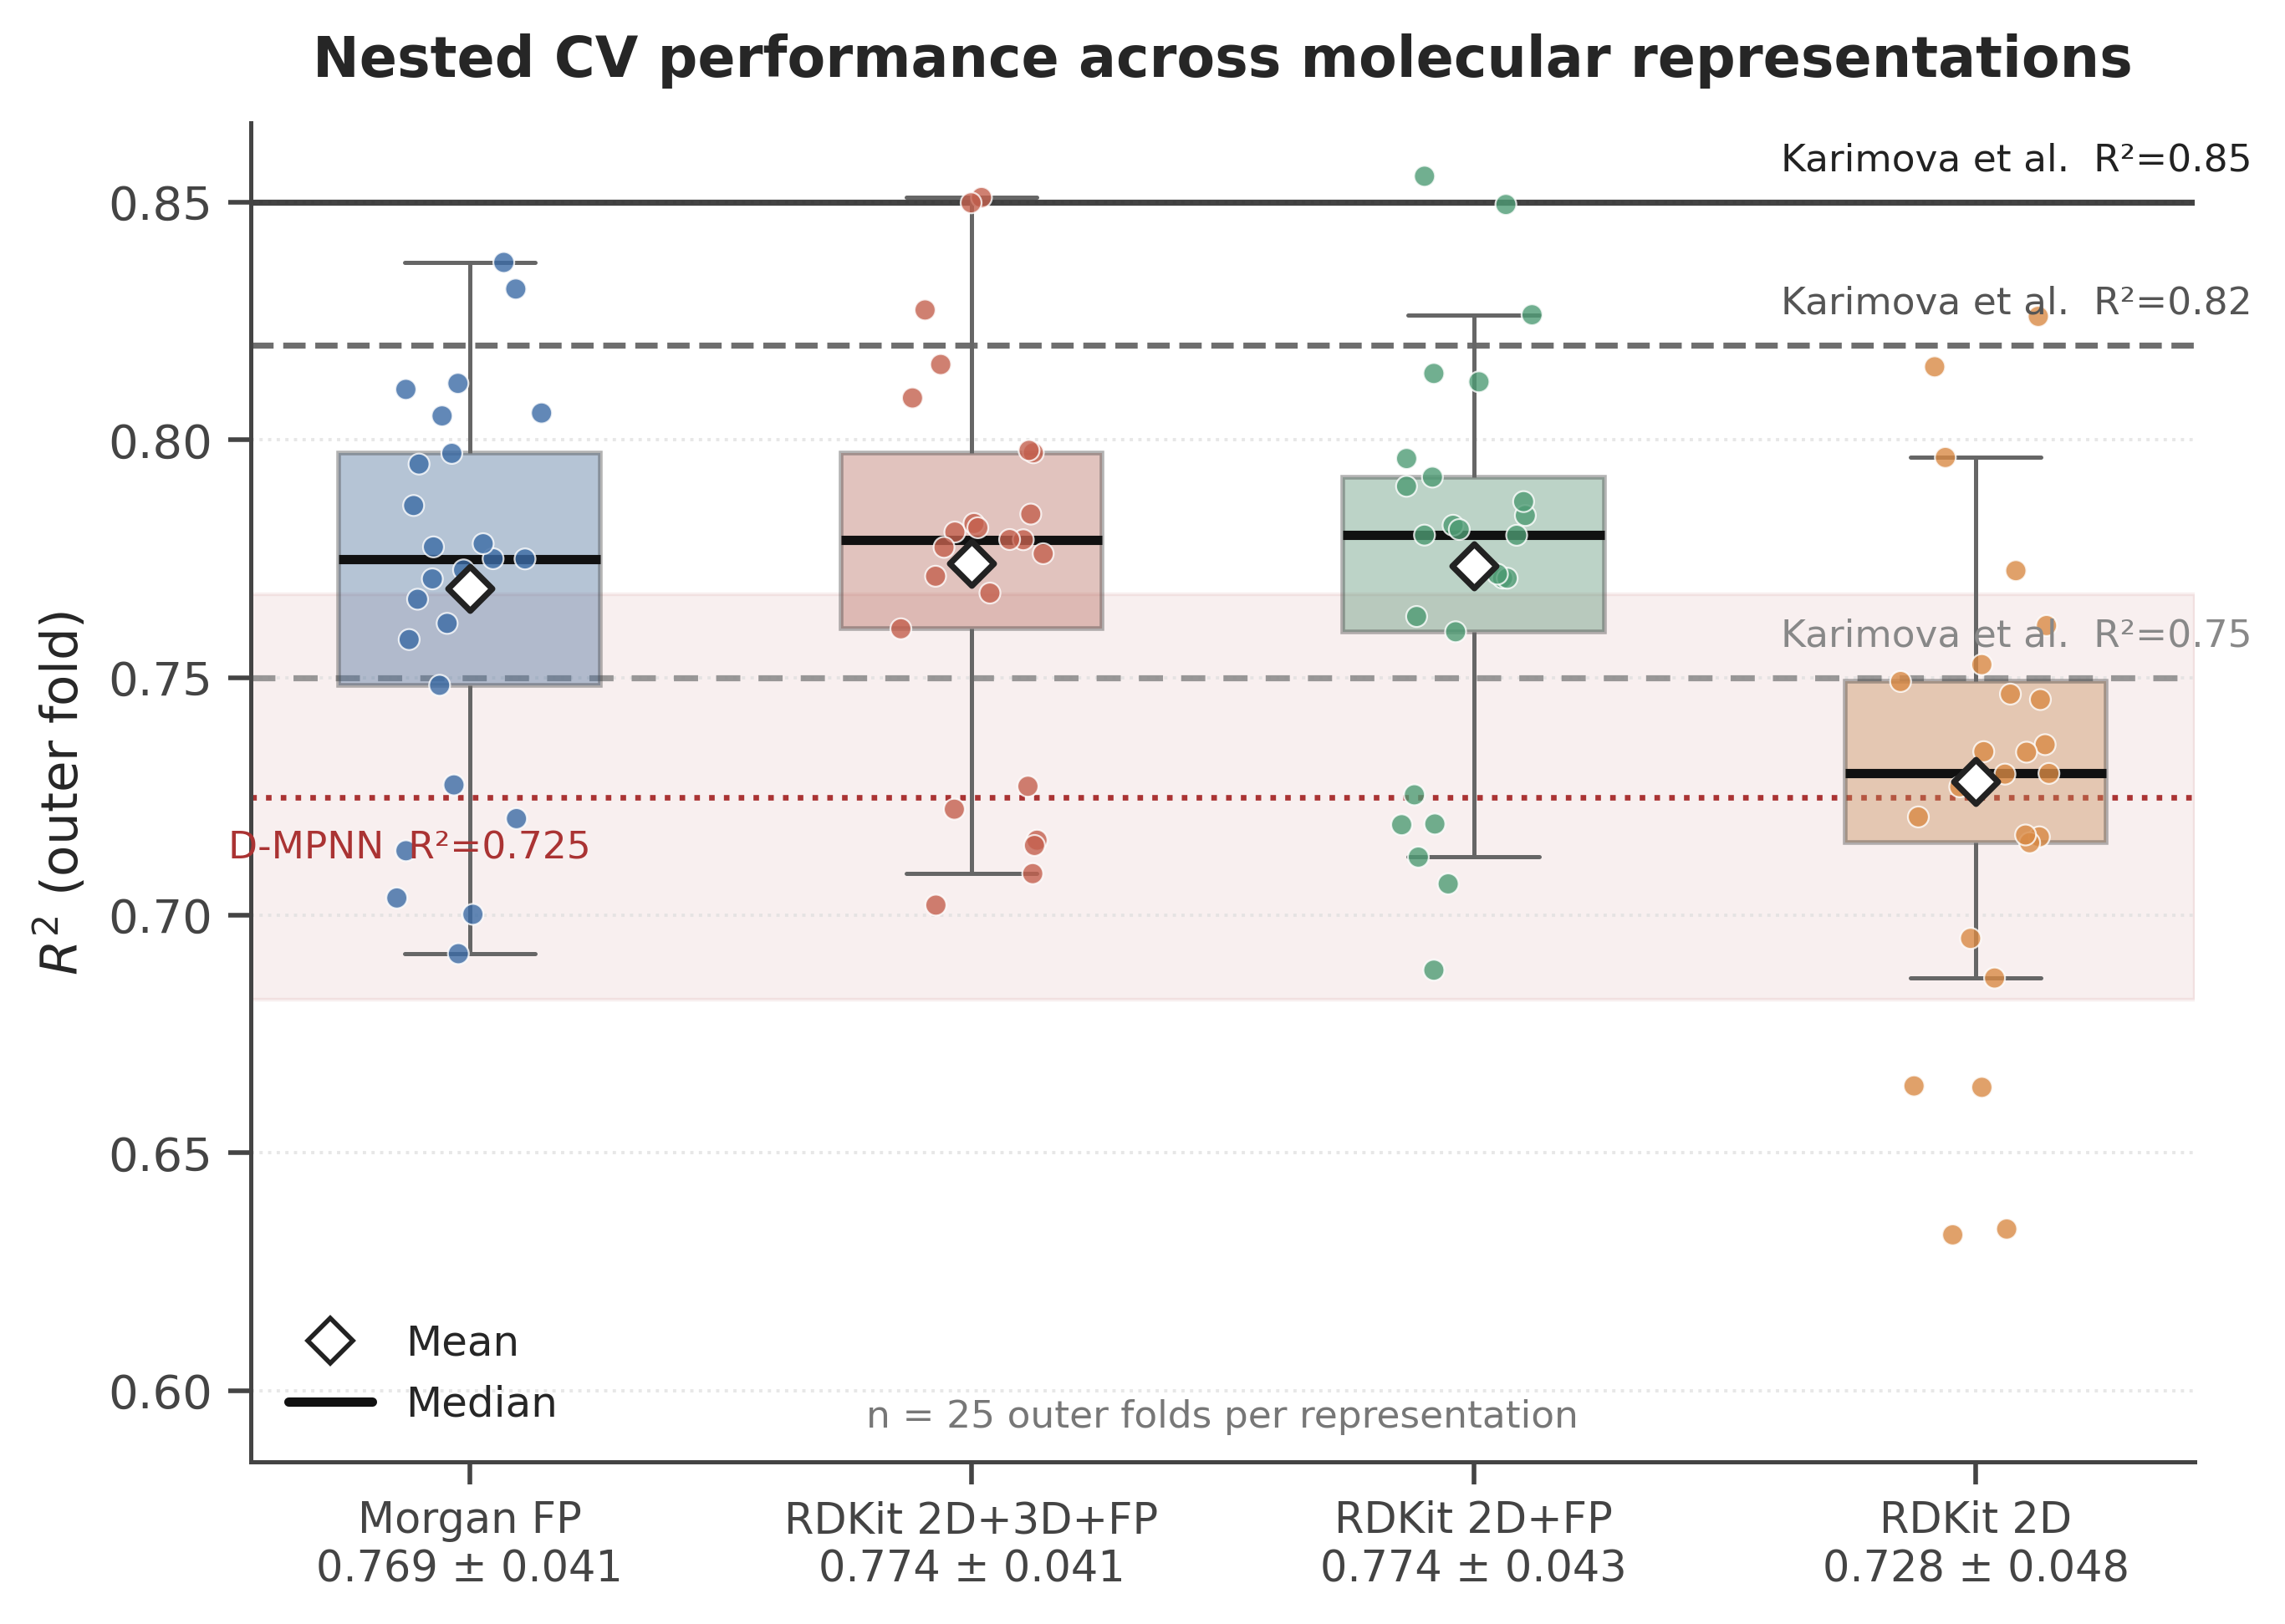
\includegraphics[width=0.8\textwidth]{figures/01_nested_cv_stability_boxplot.png}
	\caption{Nested cross-validation $R^2$ across four molecular representations (each point is one of the 25 outer folds). Horizontal lines mark the three values reported in the original study \cite{karimova2025}; the dotted line and band show the mean $\pm$ SD of the D-MPNN benchmarked in Section~\ref{sec:gnn_results}. The three representations that contain fingerprints are statistically indistinguishable in $R^2$.}
	\label{fig:nested_cv_boxplot}
\end{figure}

Differences between representations were assessed with Nadeau-Bengio corrected paired $t$-tests on the shared outer folds. The three fingerprint-containing spaces could not be separated in $R^2$ (Morgan versus 2D descriptors with fingerprints, $p = \NBpRTwoMorganVsTwoDFp$; Morgan versus the 3D hybrid, $p = \NBpRTwoMorganVsTwoDThreeDFp$; 2D descriptors with fingerprints versus the 3D hybrid, $p = \NBpRTwoTwoDFpVsTwoDThreeDFp$). In MAE, Morgan trailed the two hybrid spaces by \NBdiffMAEMorganVsTwoDFp\ and \NBdiffMAEMorganVsTwoDThreeDFp\ $pIC_{50}$ units ($p = \NBpMAEMorganVsTwoDFp$ and $p = \NBpMAEMorganVsTwoDThreeDFp$), a small gap that is no longer significant after Holm adjustment for the six comparisons ($p_{\mathrm{Holm}} = \NBpHolmMAEMorganVsTwoDFp$ for both). In contrast, 2D descriptors alone were significantly worse than every space that includes fingerprints (versus 2D descriptors with fingerprints, $p = \NBpRTwoTwoDVsTwoDFp$; versus the 3D hybrid, $p = \NBpRTwoTwoDVsTwoDThreeDFp$; versus Morgan, $p = \NBpRTwoMorganVsTwoD$). Topological fingerprints are therefore the primary driver of predictive capacity, and the ten 3D shape descriptors derived from ETKDGv3 embedding and MMFF94 minimization added no measurable advantage for this benchmark.

To rule out chance correlation, a \YRandomNPermutations-iteration y-randomization test was applied to the stacking ensemble of the screening model (\YRandomArchitecture: random forest, XGBoost and SVR with a ridge meta-learner) trained on Morgan fingerprints and scored by \YRandomCVFolds-fold cross-validation. With the true potencies this model reached $R^2 = \YRandomTrueRTwo$ (a single \YRandomCVFolds-fold partition, which explains the small difference from the nested estimate), whereas the permuted models collapsed to a mean $R^2$ of $\YRandomMeanRTwo \pm \YRandomStdRTwo$, a separation of $Z = \YRandomZScore$ standard deviations. The ensemble therefore maps genuine structure--activity relationships rather than memorizing noise.

Selection of the stacking architecture was unstable (Figure~\ref{fig:algorithm_selection}). Within the Morgan space, Support Vector Regression entered the selected ensemble in \SelMorganSVMPct\% of the outer folds and Random Forest in \SelMorganRFPct\%, followed by XGBoost (\SelMorganXGBPct\%), LightGBM (\SelMorganLGBMPct\%), $k$-nearest neighbors (\SelMorgankNNPct\%), and Extra Trees (\SelMorganETPct\%); the selected ensembles contained one, two, or three models in \SelMorganSizeOnePct\%, \SelMorganSizeTwoPct\%, and \SelMorganSizeThreePct\% of the folds. No single hierarchy dominated: the most frequent exact combination, \MorganBestArchitecture, won only \MorganStability\% of the folds (\SelMorganTopCount/\TotalOuterFolds), followed by \SelMorganSecond\ (\SelMorganSecondCount/\TotalOuterFolds) and \SelMorganNOthers\ further architectures selected in at most \SelMorganOthersMaxCount\ folds each. The descriptor-based spaces behaved differently: Extra Trees was selected in \SelRdkitTwoDETPct\%, \SelRdkitTwoDFpETPct\%, and \SelRdkitTwoDThreeDFpETPct\% of the folds of the 2D, 2D+FP, and 2D+3D+FP spaces, respectively, and SVR in \SelRdkitTwoDSVMPct\%, \SelRdkitTwoDFpSVMPct\%, and \SelRdkitTwoDThreeDFpSVMPct\%. While aggregated performance remains stable across outer folds, the data sparsity of the \NCompounds-compound benchmark prevents the inner loop from isolating a universally superior ensemble.

\begin{figure}[htbp]
	\centering
	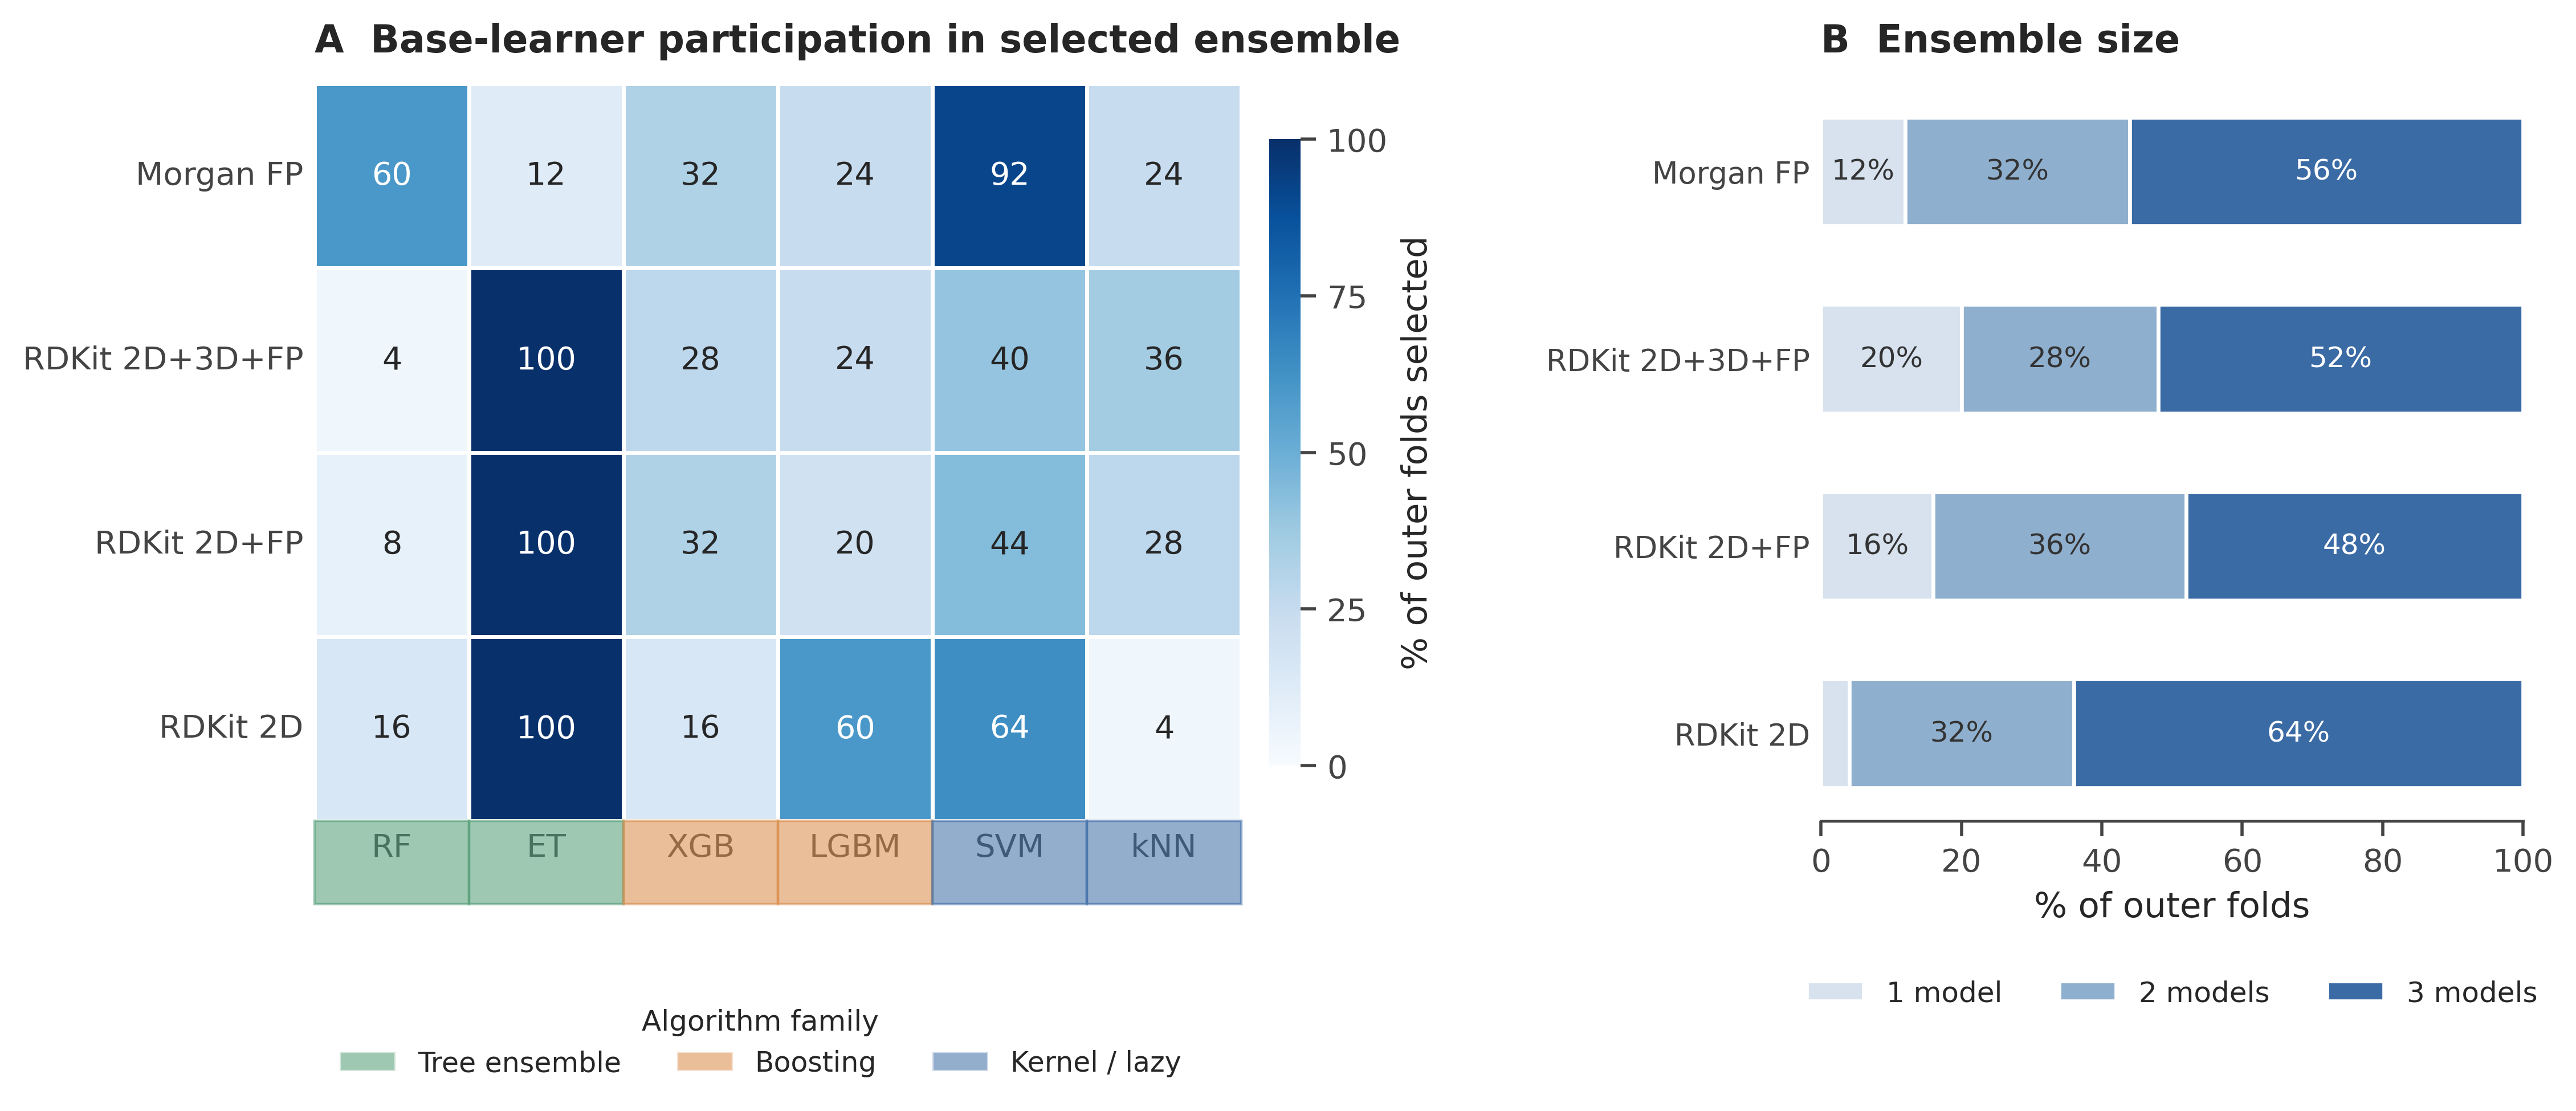
\includegraphics[width=\textwidth]{figures/01_nested_cv_algorithm_selection.png}
	\caption{Composition of the stacking ensembles selected by the inner loop in the 25 outer folds. (A) Percentage of folds in which each base learner entered the selected ensemble, per representation. (B) Distribution of ensemble size (one, two, or three base models). No single architecture dominates in the Morgan space.}
	\label{fig:algorithm_selection}
\end{figure}

We then placed these results against the incremental progression reported in the original study (Table~\ref{tab:methodological_comparison}). Our classical stacking ensemble trained solely on Morgan features ($R^2 = \MorganRTwoMean$) performed comparably to their unselected 2D/3D/FP baseline ($R^2 = \PaperBaselineRTwo$); under a Nadeau-Bengio corrected one-sample $t$-test the difference was not significant ($t = \TStatMorganVsPaperBaseline$, $p = \PValueMorganVsPaperBaseline$). In contrast, the literature value for the model with permutation-importance feature selection ($R^2 = \PaperSelectedRTwo$) lies significantly above our nested cross-validated Morgan estimate ($t = \TStatMorganVsPaperSelected$, $p = \PValueMorganVsPaperSelected$), and so does the final data-augmented deep neural network ensemble ($R^2 = \PaperFinalRTwo$; $t = \TStatMorganVsPaperFinal$, $p = \PValueMorganVsPaperFinal$). This comparison has a limitation: the original values come from a single hold-out split without a reported dispersion and are treated here as fixed constants, so the test does not capture the sampling variability of that split. Achieving a competitive baseline ($R^2 \approx \PaperBaselineRTwo$) does not require computationally expensive 3D descriptors or complex neural network architectures; simple 2D fingerprints paired with classical algorithms suffice.

\begin{table}[htbp]
	\centering
	\caption{Methodological comparison isolating the performance impact of architectural complexity, descriptor dimensionality, and data augmentation in TgDHFR bioactivity prediction.}
	\label{tab:methodological_comparison}
	\small
	\begin{tabular}{@{}>{\raggedright\arraybackslash}p{0.35\textwidth}p{0.2\textwidth}p{0.13\textwidth}p{0.2\textwidth}@{}}
		\toprule
		\textbf{Model Framework} & \textbf{Descriptors} & \shortstack[l]{\textbf{Data}\\\textbf{Augmentation}} & \shortstack[l]{\textbf{Test $R^2$}\\\textbf{(mean $\pm$ std)}} \\
		\midrule
		Current Study (Classical Ensemble) & ECFP4 (2D) & None & \MorganRTwoMean $\pm$ \MorganRTwoStd \\
		Baseline \cite{karimova2025} & 2D/3D/FP & None & \PaperBaselineRTwo \textsuperscript{a} \\
		Feature-selected model \cite{karimova2025} & 2D/3D/FP (Selected) & None & \PaperSelectedRTwo \textsuperscript{a} \\
		Augmented Final Model \cite{karimova2025} & 2D/3D/FP (Selected) & Gaussian Noise & \PaperFinalRTwo \textsuperscript{a} \\
		\bottomrule
		\multicolumn{4}{p{0.9\textwidth}}{\footnotesize \textsuperscript{a} Standard deviation not reported (NR) in the original study.}
	\end{tabular}
\end{table}

To test whether the interventions credited with the gains of the original study transfer to classical learners, we replicated its protocol (15\% hold-out, seed 42; \ExpNTest\ molecules held out before any selection or augmentation, \ExpNDev\ for development) on a stacking ensemble (Figure~\ref{fig:augmentation_ablation}). The unselected baseline reached $R^2 = \ExpARTwoMean$ (MAE = \ExpAMae). Permutation-importance selection (\ExpBNFeaturesSelected\ of \ExpBNFeaturesTotal\ bits retained) yielded $R^2 = \ExpBRTwoMean$ (MAE = \ExpBMae), and Gaussian-noise augmentation yielded $R^2 = \ExpCRTwoMean$ (MAE = \ExpCMae). Paired bootstrap differences showed no significant effect of either intervention: selection changed $R^2$ by $\ExpBvsADeltaRTwo$ (95\% CI $[\ExpBvsADeltaCILow, \ExpBvsADeltaCIHigh]$) and augmentation by $\ExpCvsADeltaRTwo$ (95\% CI $[\ExpCvsADeltaCILow, \ExpCvsADeltaCIHigh]$) relative to the baseline, and both intervals include zero. The hold-out intervals are wide, spanning roughly 0.2 $R^2$ units, and contain the original baseline of \PaperBaselineRTwo; the original values of \PaperSelectedRTwo\ and \PaperFinalRTwo\ lie above the upper limits of the intervals for selection ($p_{\mathrm{boot}} = \ExpBVsPaperSelectedPBoot$) and augmentation ($p_{\mathrm{boot}} = \ExpCVsPaperFinalPBoot$), respectively. The gains reported for the original deep ensemble were therefore not reproduced by feature selection or augmentation applied to a classical learner; they may depend on the neural architecture, or reflect the sampling variability of a single hold-out split. Two properties of the replicated interventions limit how strong this negative result is. First, the permutation importance was computed on the data the model was fitted on, so the selection removes essentially the bits the model never uses and little else, and no change is expected for tree-based learners. Second, Gaussian noise of $\sigma \leq 0.01$ added to binary fingerprint bits barely moves the split thresholds of tree models, so the augmented copies are almost identical to the originals. Neither intervention was therefore a demanding test of its idea.

\begin{figure}[htbp]
	\centering
	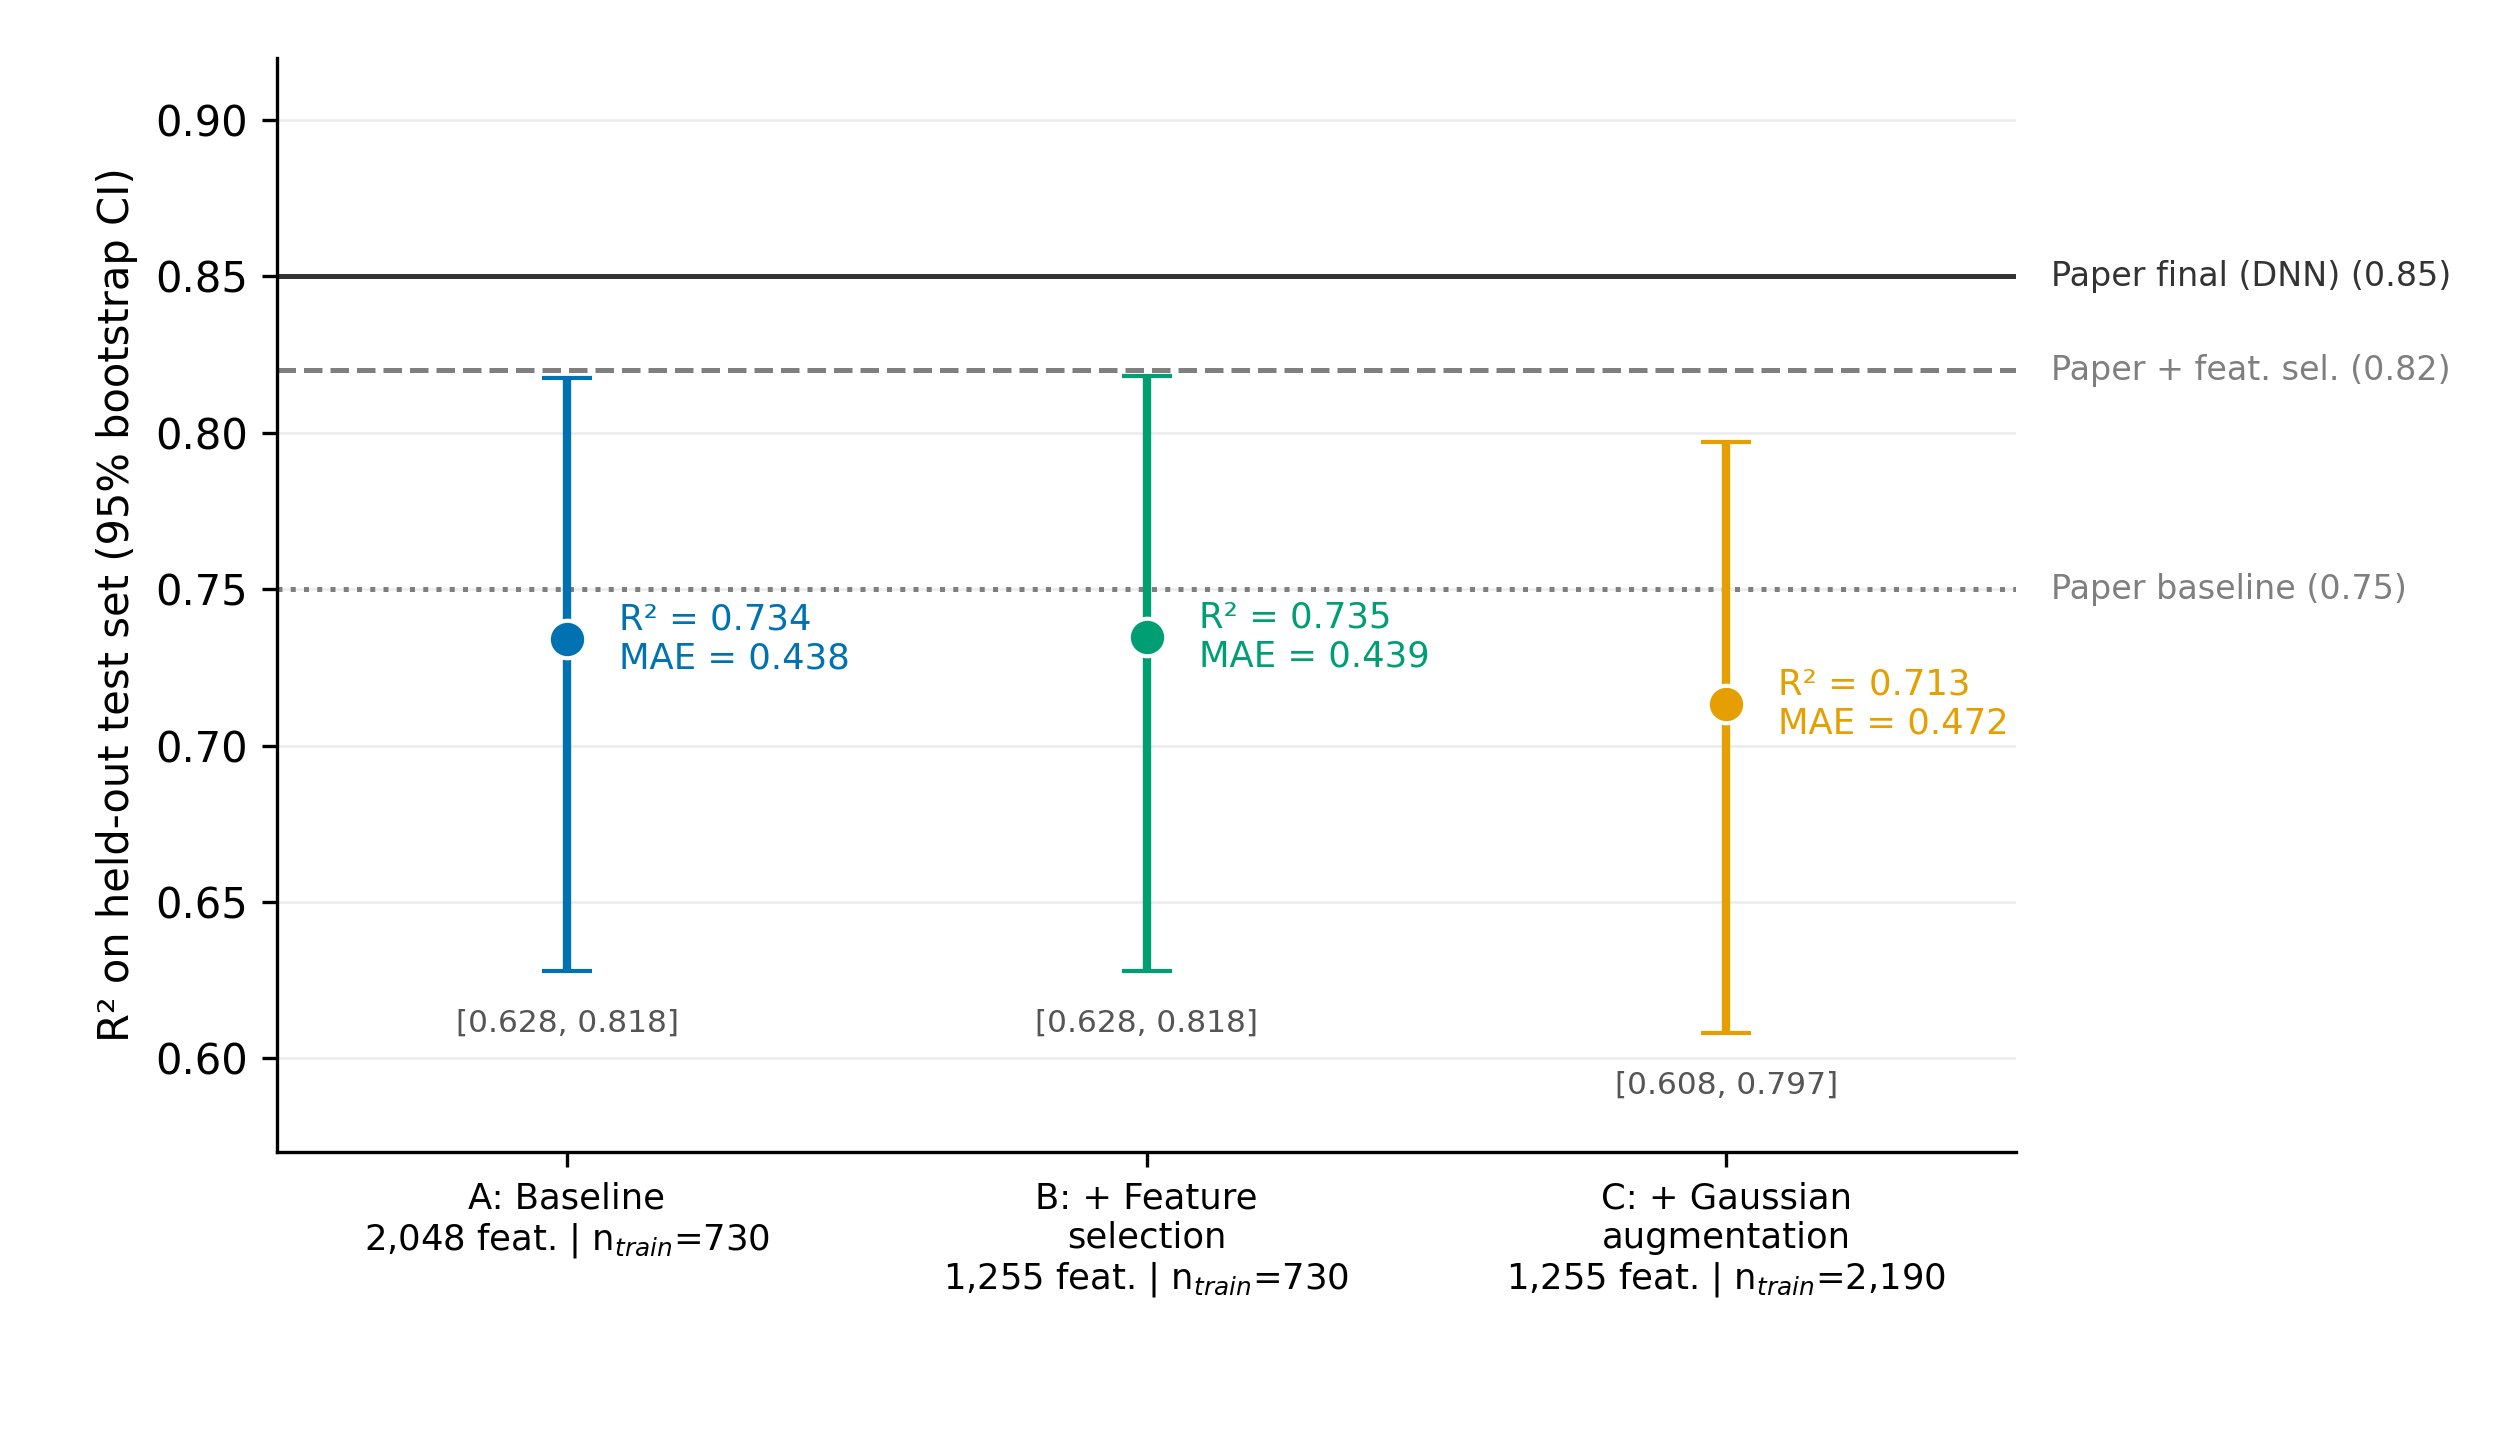
\includegraphics[width=0.8\textwidth]{figures/04_augment_r2_comparison.png}
	\caption{Replication of the original hold-out protocol on a classical stacking ensemble (\ExpNTest\ held-out molecules). Points are $R^2$ on the test set with 95\% bootstrap confidence intervals for the baseline (A), permutation-importance feature selection (B), and feature selection plus Gaussian-noise augmentation (C); horizontal lines mark the values reported in the original study \cite{karimova2025}.}
	\label{fig:augmentation_ablation}
\end{figure}

% ==========================================
% 3. SECTION 3.2
% ==========================================
\subsection{Benchmarking Tree-Based Ensembles Against Graph Neural Networks}
\label{sec:gnn_results}

Graph neural networks learn molecular representations directly from the atom--bond graph, but their advantage is expected to shrink when labeled data are scarce. To test whether representation learning helps on the TgDHFR dataset (\NCompounds\ compounds), a Directed Message Passing Neural Network (D-MPNN, Chemprop) was evaluated on exactly the same \TotalOuterFolds\ outer folds as the classical ensembles, in two variants described in the Methods: default hyperparameters, and a hyperparameter search nested inside each outer fold.

The default D-MPNN reached a mean fold $R^2$ of $\ChemPropDMPNNFoldRTwoMean \pm \ChemPropDMPNNFoldRTwoStd$ and a mean absolute error of \ChemPropDMPNNFoldMae, compared with $R^2 = \MorganRTwoMean \pm \MorganRTwoStd$ for the Morgan-fingerprint stacking ensemble (Figure~\ref{fig:gnn_comparison}). Because the folds are shared, the models can be compared with the same Nadeau--Bengio corrected paired $t$-test used for the classical representations. The network was numerically below the Morgan ensemble ($\Delta R^2 = \GnnVsMorganDiffRTwo$) and the fingerprint-based hybrid ensembles ($\Delta R^2 = \GnnVsRdkitTwoDFpDiffRTwo$ and $\GnnVsRdkitTwoDThreeDFpDiffRTwo$ against 2D+FP and 2D+3D+FP), and on par with the 2D descriptors alone ($\Delta R^2 = \GnnVsRdkitTwoDDiffRTwo$), but no difference was significant after Holm adjustment (smallest adjusted $p$: \GnnVsMinPRTwo\ for $R^2$ and \GnnVsMinPMae\ for MAE).

Tuning did not change this picture. In the nested search, the selected configuration varied across folds (\GnnTunedNChosen\ of the \GnnTunedNConfigs\ configurations were chosen at least once, and the default one in only \GnnTunedDefaultChosenPct\% of the folds), but the tuned network reached $R^2 = \GnnTunedRTwoMean \pm \GnnTunedRTwoStd$ and MAE = \GnnTunedMae, indistinguishable from the default one ($\Delta R^2 = \GnnTunedVsUntunedDiffRTwo$, $p = \GnnTunedVsUntunedPRTwo$; $\Delta$MAE $= \GnnTunedVsUntunedDiffMae$, $p = \GnnTunedVsUntunedPMae$). Against the classical ensembles the tuned network was again numerically lower than Morgan ($\Delta R^2 = \GnnTunedVsMorganDiffRTwo$, Holm-adjusted $p = \GnnTunedVsMorganPRTwo$) and the two fingerprint-based hybrids ($\Delta R^2 = \GnnTunedVsRdkitTwoDFpDiffRTwo$ and $\GnnTunedVsRdkitTwoDThreeDFpDiffRTwo$), and on par with the 2D descriptors ($\Delta R^2 = \GnnTunedVsRdkitTwoDDiffRTwo$); none of these differences was significant (smallest adjusted $p$: \GnnTunedVsMinPRTwo\ for $R^2$ and \GnnTunedVsMinPMae\ for MAE).

Equivalence is a separate question. With the $\pm 0.05$ margin, the tuned network was equivalent to the 2D descriptors in $R^2$ (90\% CI $[\GnnTunedVsRdkitTwoDCILowRTwo, \GnnTunedVsRdkitTwoDCIHighRTwo]$, $p = \GnnTunedVsRdkitTwoDEquivPRTwo$), but equivalence to the Morgan ensemble could not be shown for $R^2$ (90\% CI $[\GnnTunedVsMorganCILowRTwo, \GnnTunedVsMorganCIHighRTwo]$, $p = \GnnTunedVsMorganEquivPRTwo$). In MAE, the tuned network and the Morgan ensemble were equivalent within $\pm 0.05$ ($\Delta = \GnnTunedVsMorganDiffMae$, 90\% CI $[\GnnTunedVsMorganCILowMae, \GnnTunedVsMorganCIHighMae]$, $p = \GnnTunedVsMorganEquivPMae$). The evidence therefore supports that the network is not clearly worse in absolute error, but leaves open a deficit in $R^2$ as large as $\Delta R^2 = \GnnTunedVsMorganCILowRTwo$. The tuned search was deliberately modest (Methods), so a larger search or a different architecture could change this.

Both graph-network variants and the classical ensembles fall in the same range as the original study's unselected baseline ($R^2 = \PaperBaselineRTwo$). The final augmented ensemble of the original study ($R^2 = \PaperFinalRTwo$) lies above this range, but, as discussed in Section~\ref{sec:res_classical}, that value comes from a single hold-out split and was not reproduced by selection or augmentation on a classical learner. Under the data volume of this benchmark, the graph architecture therefore did not provide a measurable gain over fixed fingerprints.

Computational cost does not favor the classical approach in this protocol, but the comparison needs care (Table~\ref{tab:cost}). One default D-MPNN training took about \GnnFoldSecMean\ s on the workstation CPU (about \GnnTotalMin\ minutes for the \TotalOuterFolds\ folds), whereas a classical outer fold with its complete inner search took between \ClassicalFoldSecMin\ and \ClassicalFoldSecMax\ s depending on the representation (\ClassicalMorganFoldSec\ s, about \ClassicalMorganTotalHours\ h in total, for Morgan). The default network received no model selection. When it did, in the tuned variant, one outer fold took \GnnTunedFoldSecMean\ s, about \GnnTunedTotalHours\ h of worker time for the whole benchmark, which is more than the classical protocol even though the network's search was smaller. The case for the classical ensembles therefore rests on accuracy that is not lower, on simpler inputs and models that run on a CPU, and on a deployed model that uses only a subset of the fingerprint bits, and not on a shorter benchmark.

\begin{table}[htbp]
	\centering
	\caption{Run time and accuracy of every model. Time is the mean wall-clock time of one outer fold on the workstation, including the inner search where one exists, and the 25-fold total is that time multiplied by 25. Times are not normalized by thread count (the classical models used all threads on one fold at a time; the tuned D-MPNN ran two training processes in parallel).}
	\label{tab:cost}
	\resizebox{\textwidth}{!}{% Auto-generated by 09.1_build_figures.py
\begin{tabular}{lcccc}
\toprule
\textbf{Model} & \textbf{Time per outer fold (s)} & \textbf{25 folds (h)} & \textbf{Model selection} & $R^2$ \\
\midrule
Morgan FP & 1987 & 13.8 & Yes (41 combinations) & $0.769 \pm 0.041$ \\
RDKit 2D+FP & 2504 & 17.4 & Yes (41 combinations) & $0.774 \pm 0.043$ \\
RDKit 2D+3D+FP & 2586 & 18.0 & Yes (41 combinations) & $0.774 \pm 0.041$ \\
RDKit 2D & 1182 & 8.2 & Yes (41 combinations) & $0.728 \pm 0.048$ \\
D-MPNN, default & 179 & 1.2 & No & $0.725 \pm 0.043$ \\
D-MPNN, tuned & 2192 & 15.2 & Yes (8 configurations) & $0.726 \pm 0.034$ \\
\bottomrule
\end{tabular}
}
\end{table}

\begin{figure}[htbp]
	\centering
	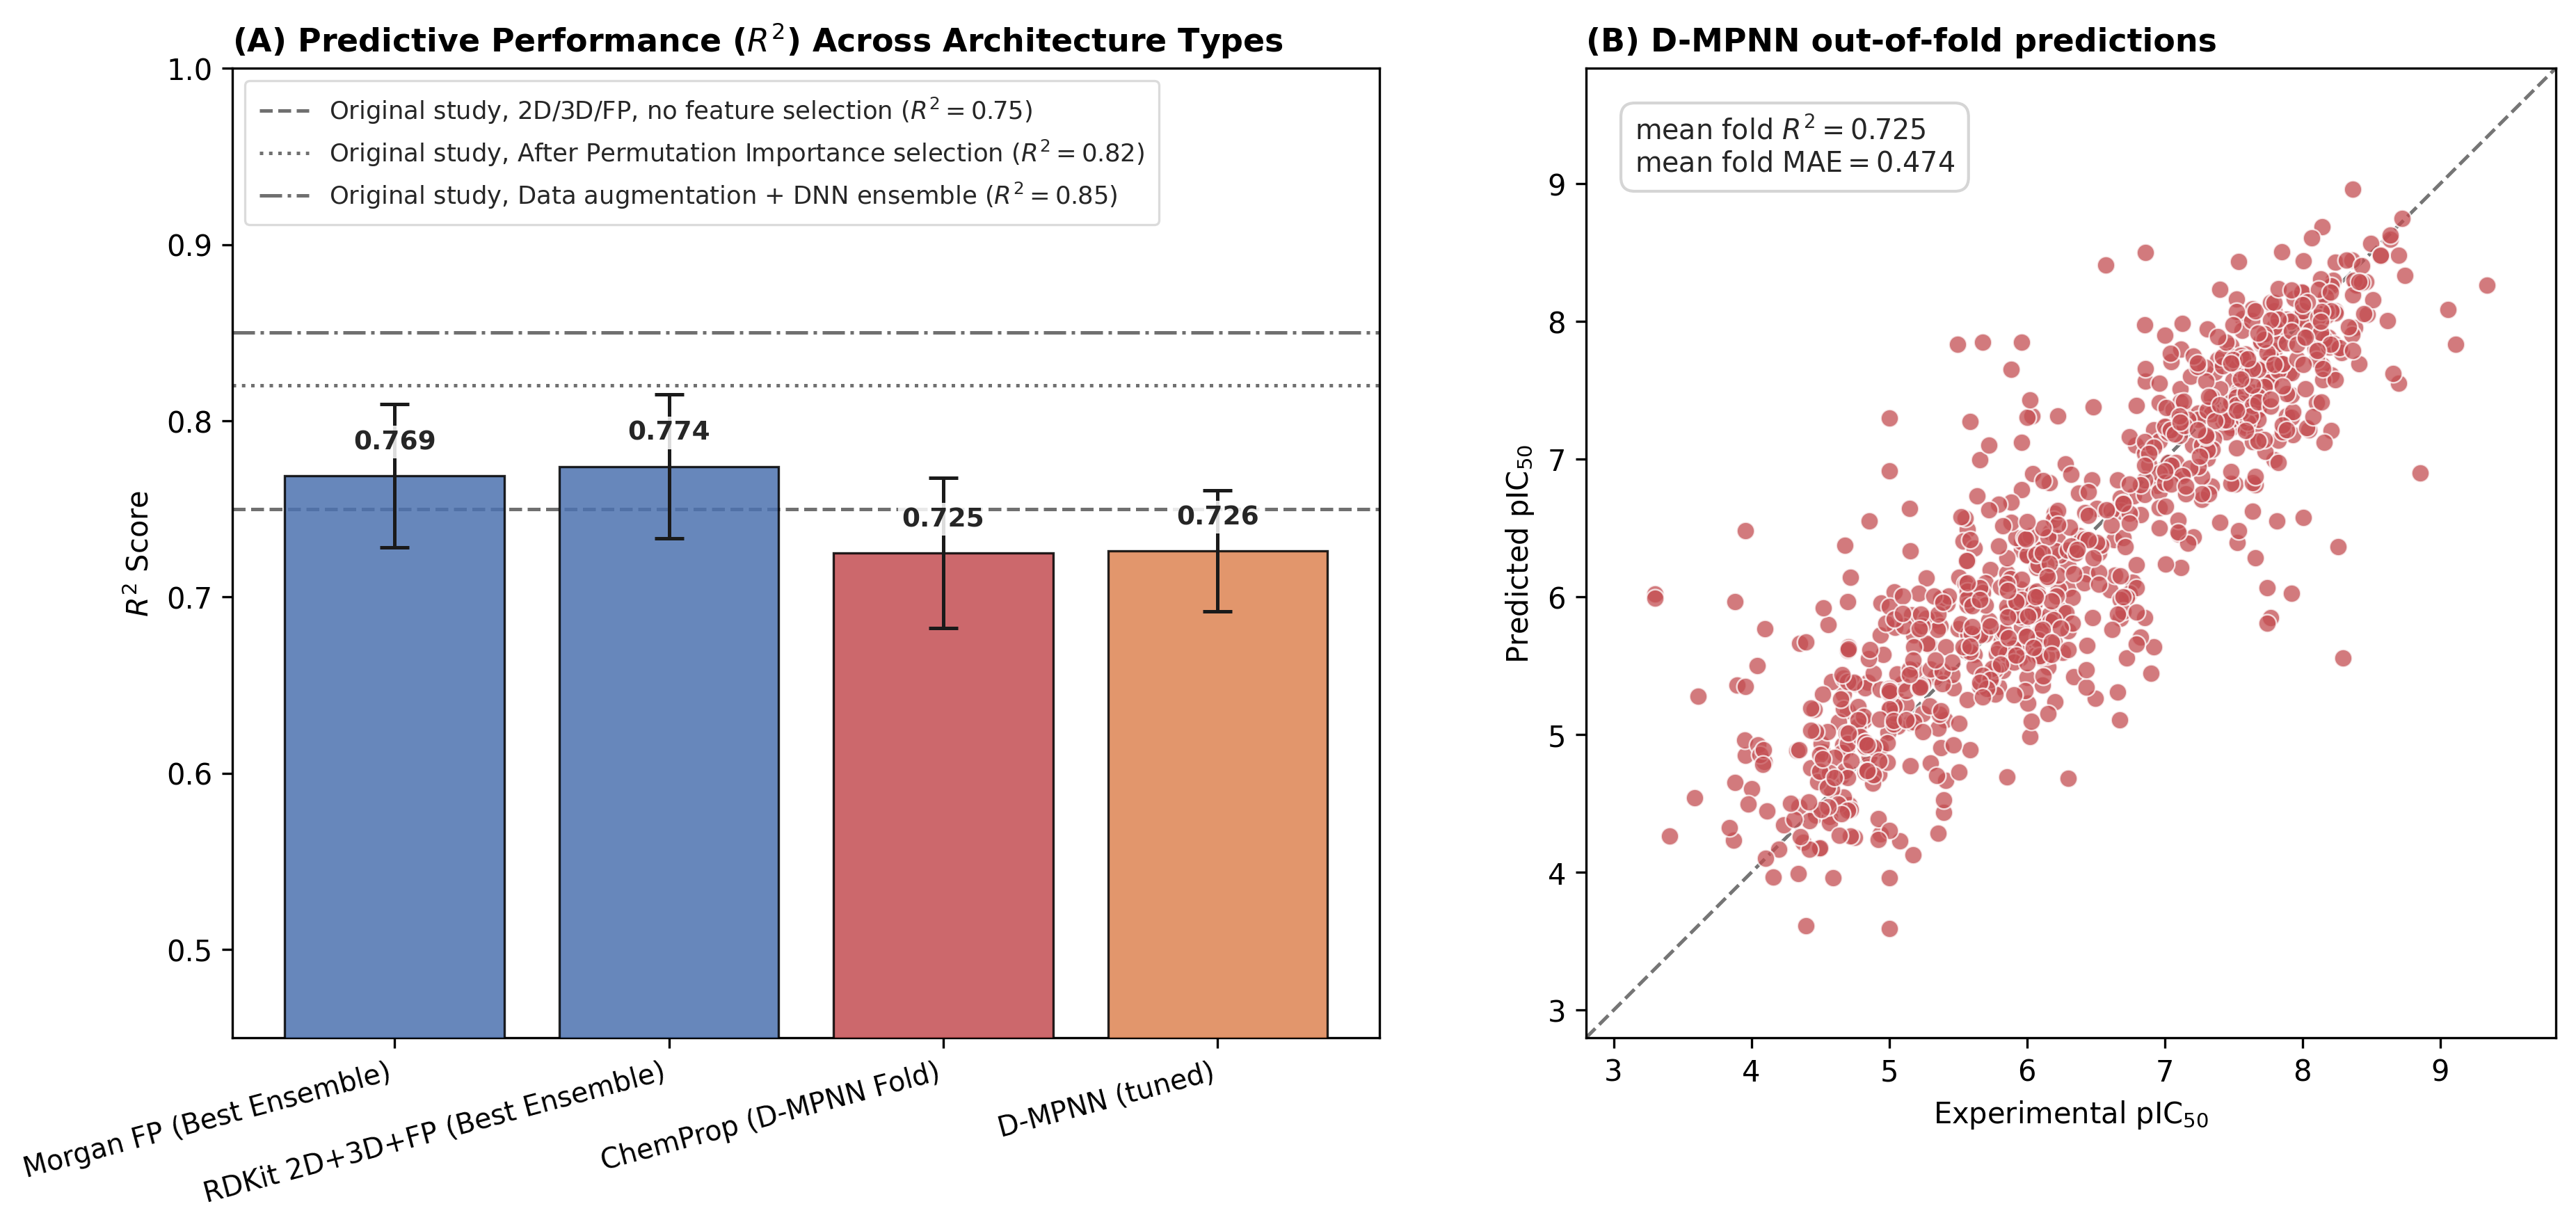
\includegraphics[width=\textwidth]{figures/09_gnn_benchmark_comparison.png}
	\caption{(A) Mean $R^2$ over the \TotalOuterFolds\ shared outer folds for the best classical ensembles and the D-MPNN with default and tuned hyperparameters; error bars are the standard deviation across folds, and horizontal lines mark the values reported in the original study. (B) Default D-MPNN predicted versus experimental pIC$_{50}$ for every compound, averaged over the five repeats of the cross-validation (each prediction comes from a model that did not see the compound).}
	\label{fig:gnn_comparison}
\end{figure}

% ==========================================
% 3. SECTION 3.3 (screening, docking and ADMET: hypothesis generation)
% ==========================================
\subsection{Hypothesis Generation: Screening, Docking and ADMET}
\label{sec:screening_results}
\label{sec:consensus_results}
\label{sec:admet_results}

The deployed model, the feature-selected Morgan-fingerprint stacking ensemble of the augmentation experiment (Section~\ref{sec:res_classical}), was applied to the FDA-approved library after the funnel described in the Methods: \ScreenNLibrary{} compounds were reduced to \ScreenNStructural{} by the size and elemental filters, and all of these were scored. Their mean Tanimoto similarity to the five most similar training compounds had a median of \ScreenADFdaMedian{} (5th--95th percentile \ScreenADFdaLow{}--\ScreenADFdaHigh{}), against \ScreenADTrainMedian{} for the training compounds measured against each other, and only \ScreenNDomain{} of them reached the applicability-domain threshold of \ScreenADMinSimilarity{}. The predicted potencies of this library are therefore mostly extrapolations, and each candidate's similarity to the training set is reported with its prediction; of the \ScreenNCandidates{} candidates advanced to docking, \ScreenNCandidatesInDomain{} were inside the domain. As a consistency check, pyrimethamine was predicted at pIC$_{50}$ \ControlPyrimethaminePred{} (experimental \ControlPyrimethamineExp{}) and trimethoprim at \ControlTrimethoprimPred{} (experimental \ControlTrimethoprimExp{}); both belong to the training partition, so this verifies that the final model fits its training data and says nothing about generalization.

Table~S1 and Figures~S3--S5 give the ranking with its efficiency metrics. The antifolates methotrexate, trimetrexate and pralatrexate lead by absolute potency, but potency scales with molecular size and their efficiency is modest (ligand efficiency between \AntifolateLEMin{} and \AntifolateLEMax{}, against the value of 0.30 commonly taken as the lower bound of a good lead); methotrexate is also in the training set, so its rank partly reflects memorization. Size-corrected metrics reorder the list: triamterene, which is absent from the training data, combines a predicted pIC$_{50}$ of \CandTriamterenePred{} with the highest ligand efficiency (\CandTriamtereneLE{}) and binding efficiency index (\CandTriamtereneBEI{}) of the table, and is therefore the clearest repurposing hypothesis of the ML stage.

Because neither ligand-based prediction nor docking is reliable alone, the \DockNTotal{} candidates were scored by both and classified by agreement (Figure~\ref{fig:docking_scatter}), a compound being a consensus hit when the model predicts it active ($pIC_{50} > \DockMLActiveThresh$) and it docks favorably ($\Delta G < \DockActiveThresh\text{ kcal/mol}$). This yielded \DockNValidated{} entries (\DockNValidatedUnique{} unique compounds): pralatrexate ($pIC_{50} = \PralatrexateMLpIC$, $\Delta G = \PralatrexateDockScore$ kcal/mol, the best docking score of the set), methotrexate (\MethotrexateMLpIC, \MethotrexateDockScore), trimetrexate glucuronate (\TrimetrexateMLpIC, \TrimetrexateDockScore) and triamterene (\TriamtereneMLpIC, \TriamtereneDockScore). Agreement between the two methods is weak: Spearman's rank correlation between predicted $pIC_{50}$ and Vina score was $\rho = \DockSpearmanRho$ ($p = \DockSpearmanP$), with the expected sign but no statistical significance, and the estimate is less informative than its $N = \DockNTotal$ suggests, because the four trimethoprim entries share one structure and one docking score. We therefore read the correlation only as evidence that docking does not reproduce the ML ranking.

The discordant cases bound both methods. Pyrimethamine, an established TgDHFR inhibitor, docked at only $\Delta G = \PyrimethamineDockScore$ kcal/mol and trimethoprim similarly ($\Delta G = \TrimethoprimDockScore$ kcal/mol); small ligands obtain modest Vina scores because the score grows with the number of contacts, which points to a limited sensitivity of the scoring function for small inhibitors rather than to an ML artifact. Bisacodyl is the opposite case, favored by docking ($\Delta G = \BisacodylDockScore$ kcal/mol) while the model predicted $pIC_{50} = \BisacodylMLpIC$; it carries none of the diaminopyrimidine-like features of the antifolate ligands in the training set, so a docking artifact of a flexible, hydrophobic ligand is the more plausible explanation. Without experimental data we cannot arbitrate between the two methods.

\begin{figure}[htbp]
	\centering
	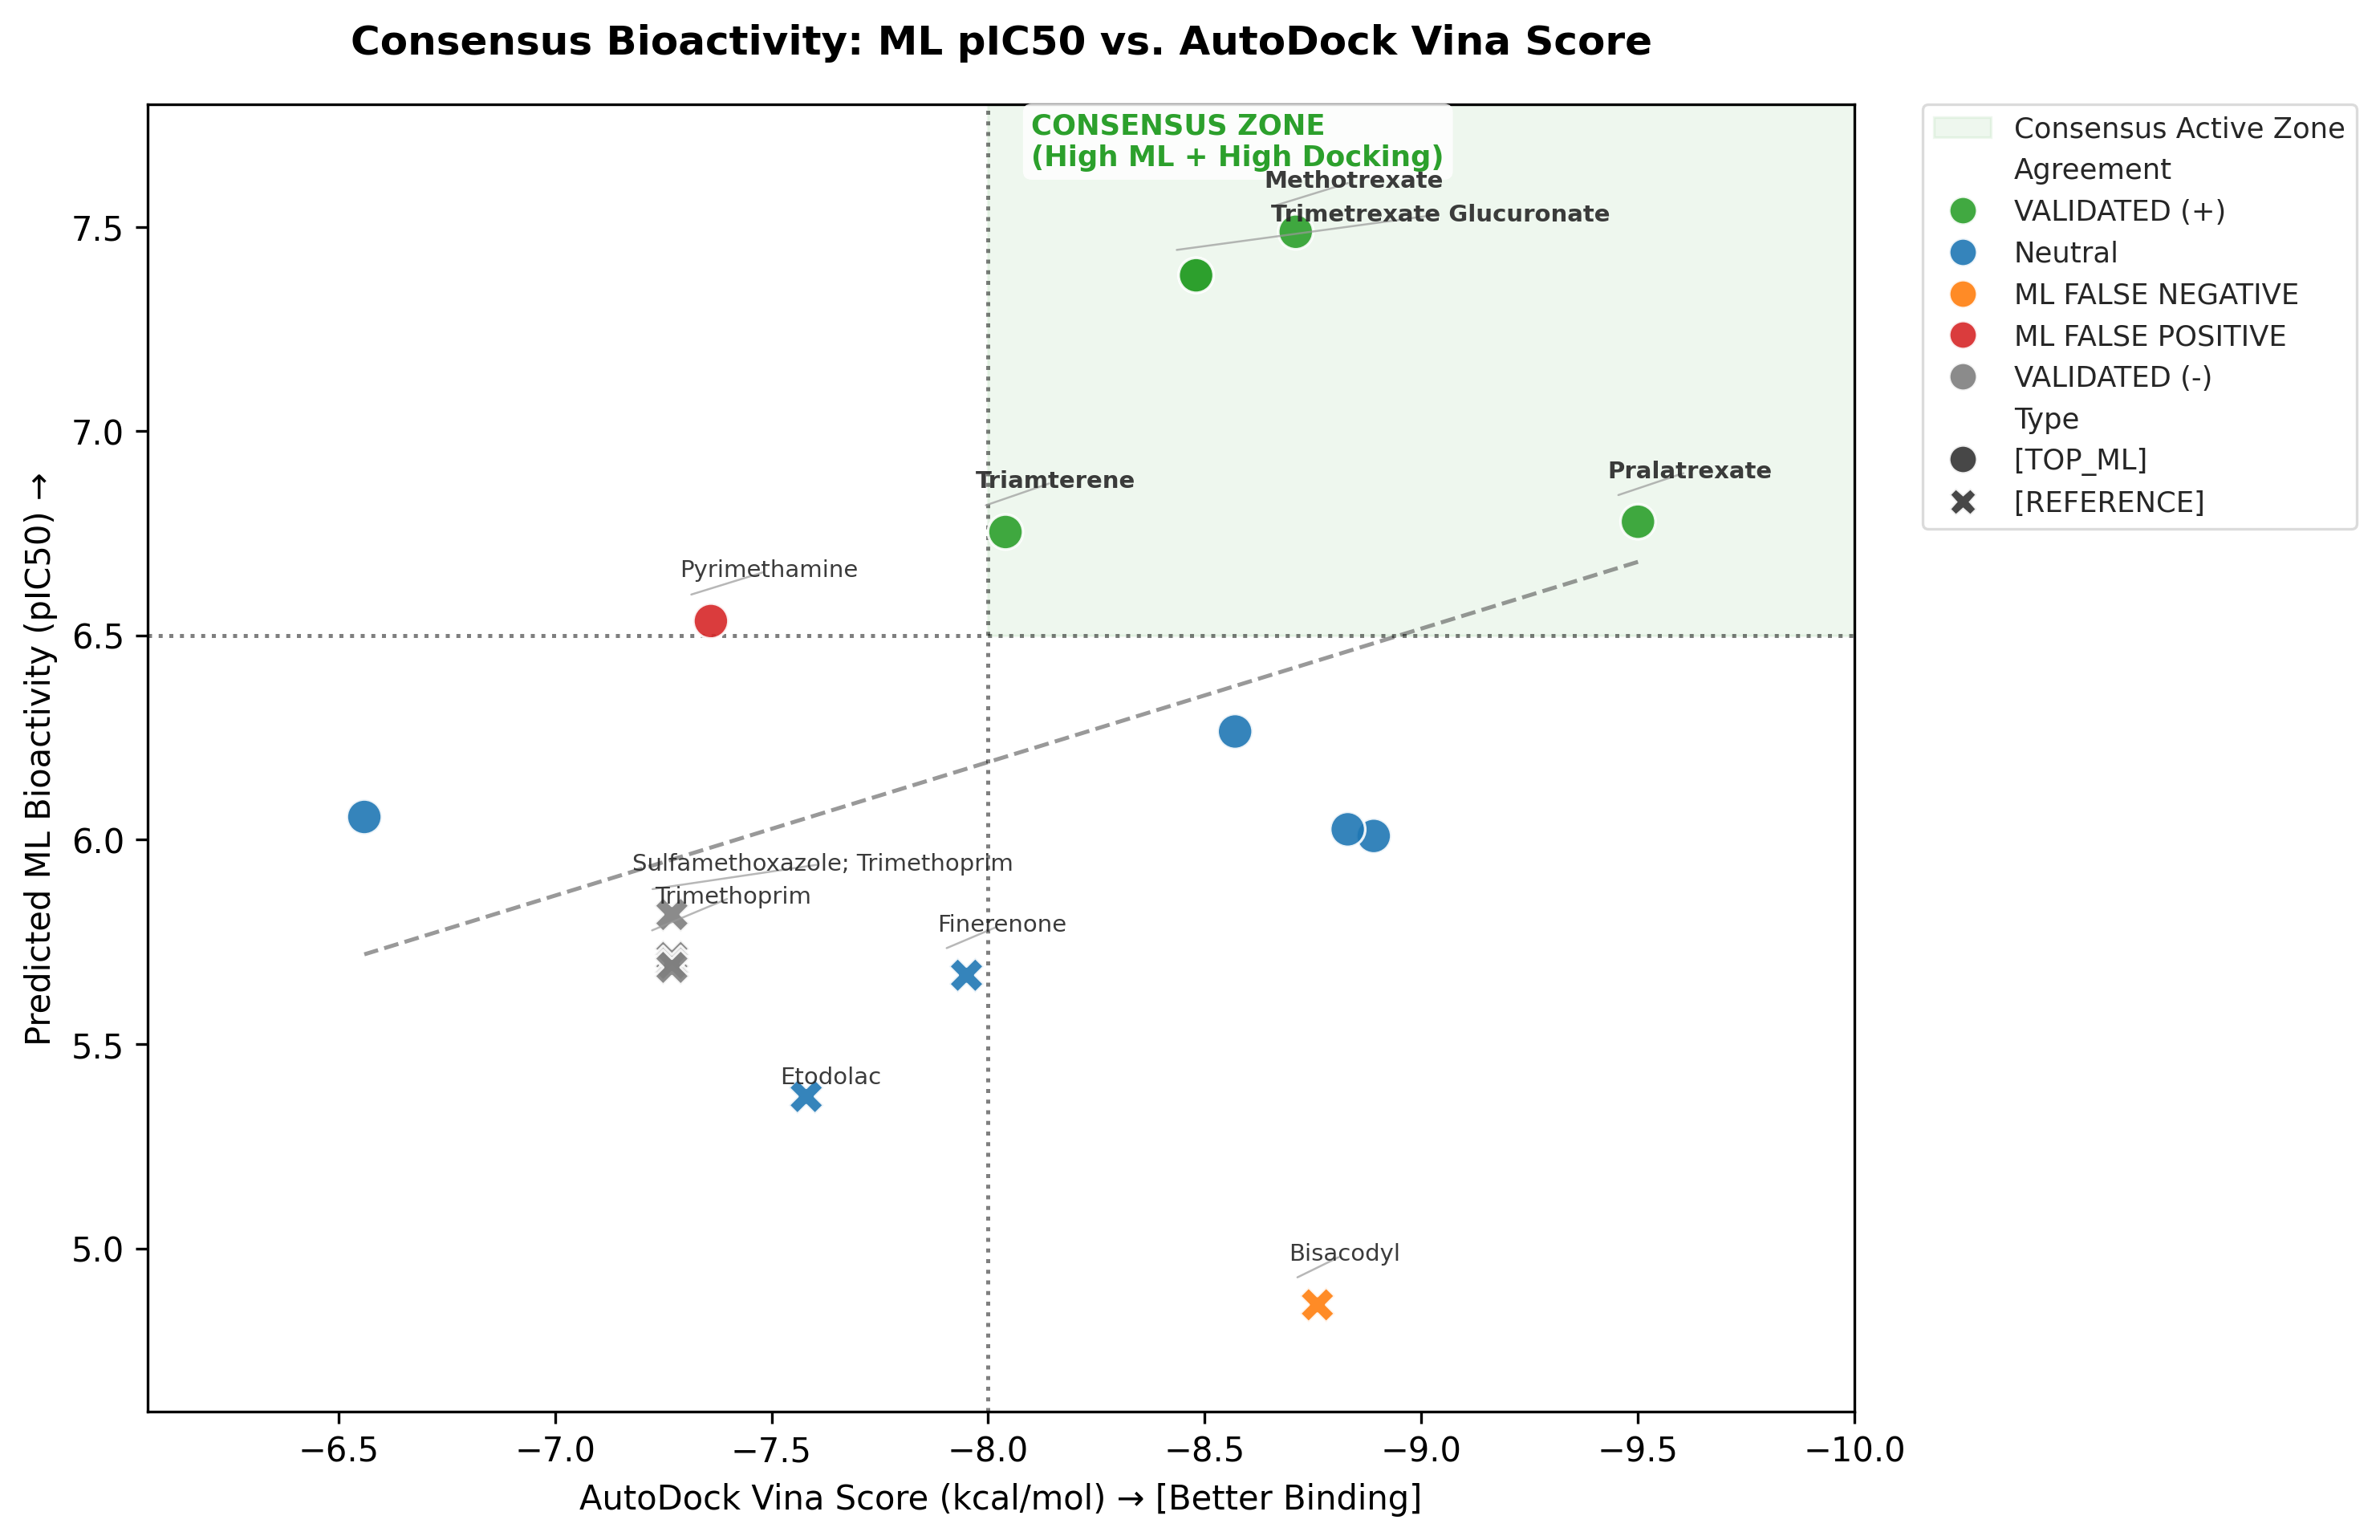
\includegraphics[width=0.9\textwidth]{figures/07_docking_scatter.png}
	\caption{Predicted pIC$_{50}$ versus AutoDock Vina score for the \DockNTotal{} docked candidates, coloured by agreement class. The shaded region is the consensus zone ($pIC_{50} > \DockMLActiveThresh$ and $\Delta G < \DockActiveThresh$ kcal/mol).}
	\label{fig:docking_scatter}
\end{figure}

Of the \AdmetNDocked{} docked entries, \AdmetNLipinski{} satisfied the three Lipinski criteria, the hERG classifier flagged \AdmetNHergFlagged{} as likely channel blockers, and \AdmetNRemaining{} remained: \AdmetNOral{} classified as oral and \AdmetNParenteral{} as parenteral because of low predicted Caco-2 permeability (Table~S2, Figure~S6). Of the \AdmetNConsensus{} consensus hits, \AdmetNConsensusSurvivors{} passed both filters: pralatrexate and methotrexate were hERG-safe but poorly permeable and so classified as parenteral, and trimetrexate was predicted to be hERG-safe and orally absorbed, whereas triamterene, the most ligand-efficient candidate of the screen, was the only consensus hit removed (predicted hERG probability \AdmetHergTriamterene{}). How much weight such a profile deserves depends on the indication and the length of the course: toxoplasmosis is treated for weeks, far longer in ocular and immunocompromised cases, and its cerebral and congenital forms require passage of the blood--brain barrier and the placenta, so the filter is informative for this target, but it is a rule- and classifier-based screen and not part of the benchmark.

This whole stage is a computational prioritization. The receptor is rigid, no water molecules or protonation states are modelled, Vina scores are empirical estimates, and the ADMET classifiers were trained on public data whose accuracy was not evaluated here, with some of these compounds in their training sets. The consensus hits are therefore hypotheses for experimental testing and not confirmed inhibitors.

% ==========================================
% 3. SECTION 3.6
% ==========================================
\subsection{Robustness to Scaffold-Grouped Splits}
\label{sec:scaffold_results}

Random folds place close analogs of a test compound in the training set, which favors models that memorize local structure. To measure how much of the reported accuracy depends on this, the Morgan-fingerprint ensemble and the D-MPNN were re-evaluated with scaffold-grouped outer folds (Section~\ref{sec:materials_ncv}), keeping the \TotalOuterFolds\ folds, the hyperparameters and the shared partitions. Table~\ref{tab:scaffold} summarizes the outcome.

\begin{table}[htbp]
	\centering
	\caption{Cross-validated performance (mean $\pm$ SD over \TotalOuterFolds\ outer folds) under random and scaffold-grouped splits. The drop is the difference in mean $R^2$.}
	\label{tab:scaffold}
	\begin{tabular}{lcccc}
		\hline
		Model & $R^2$ (random) & $R^2$ (scaffold) & Drop in $R^2$ & MAE (scaffold) \\
		\hline
		Morgan ensemble & $\RandomMorganRTwoMean \pm \RandomMorganRTwoStd$ & $\ScaffoldMorganRTwoMean \pm \ScaffoldMorganRTwoStd$ & \ScaffoldMorganDropRTwo & \ScaffoldMorganMae \\
		D-MPNN & $\RandomGnnRTwoMean \pm \RandomGnnRTwoStd$ & $\ScaffoldGnnRTwoMean \pm \ScaffoldGnnRTwoStd$ & \ScaffoldGnnDropRTwo & \ScaffoldGnnMae \\
		\hline
	\end{tabular}
\end{table}

Both families lost about 0.2 units of $R^2$ when scaffolds were held out: from $\RandomMorganRTwoMean$ to $\ScaffoldMorganRTwoMean$ for the Morgan ensemble (MAE from \RandomMorganMae\ to \ScaffoldMorganMae) and from $\RandomGnnRTwoMean$ to $\ScaffoldGnnRTwoMean$ for the D-MPNN (MAE from \RandomGnnMae\ to \ScaffoldGnnMae). The fold-to-fold spread also more than doubled (SD of $R^2$ from \RandomMorganRTwoStd\ to \ScaffoldMorganRTwoStd\ and from \RandomGnnRTwoStd\ to \ScaffoldGnnRTwoStd, respectively), because the difficulty of a fold now depends on which scaffolds it contains. The random-split estimates of the main benchmark therefore overstate the performance expected on new chemotypes.

The comparison between families kept its direction but not its resolution. Under scaffold splits the D-MPNN was lower than the Morgan ensemble by $\Delta R^2 = \ScaffoldGnnVsMorganDiffRTwo$ (corrected $p = \ScaffoldGnnVsMorganPRTwo$, Holm-adjusted; $\Delta$MAE $= \ScaffoldGnnVsMorganDiffMae$, $p = \ScaffoldGnnVsMorganPMae$). The 90\% confidence interval of the $R^2$ difference, $[\ScaffoldGnnVsMorganCILowRTwo, \ScaffoldGnnVsMorganCIHighRTwo]$, includes zero but also extends beyond the $\pm 0.05$ equivalence margin, and the equivalence test was not significant ($p = \ScaffoldGnnVsMorganEquivPRTwo$). With the present data we can thus neither claim a difference nor equivalence between the two families on new scaffolds; the sample (\NCompounds\ compounds) is too small to separate them given the larger variance of this protocol.

% ==========================================
% 3. SECTION 3.7
% ==========================================
\subsection{Sensitivity to Extreme Potency Values}
\label{sec:outlier_sensitivity}

The two records excluded by the Tukey rule (Section~\ref{sec:materials_curation}) were retained in a second, complete execution of the nested cross-validation benchmark ($n = \OutlierNSens$ versus $n = \OutlierNMain$ in the primary analysis; identical algorithms, search space and 5$\times$5 protocol). If these records were informative members of the chemical series, retaining them should not degrade generalization; if they are outliers, retaining them should lower accuracy. Table~\ref{tab:outlier_sensitivity} reports the outcome.

\begin{table}[htbp]
	\centering
	\caption{Nested cross-validation performance without (primary analysis, $n = \OutlierNMain$) and with ($n = \OutlierNSens$) the two extreme-potency records. $p$-values compare the two runs with a Welch test using the Nadeau-Bengio variance correction \cite{nadeau2003}; the runs use different fold partitions, so folds are not paired.}
	\label{tab:outlier_sensitivity}
	% Auto-generated by 10_outlier_sensitivity.py
\begin{tabularx}{\textwidth}{>{\raggedright\arraybackslash}Xcccccccc}
\toprule
& \multicolumn{4}{c}{\textbf{$R^2$}} & \multicolumn{4}{c}{\textbf{MAE}} \\
\cmidrule(lr){2-5} \cmidrule(lr){6-9}
\textbf{Representation} & Without & With & $\Delta$ & $p$ & Without & With & $\Delta$ & $p$ \\
\midrule
RDKit 2D+3D FP & 0.774 & 0.754 & -0.020 & 0.52 & 0.428 & 0.440 & +0.012 & 0.62 \\
RDKit 2D FP & 0.774 & 0.753 & -0.020 & 0.53 & 0.428 & 0.439 & +0.011 & 0.64 \\
Morgan FP & 0.769 & 0.750 & -0.019 & 0.56 & 0.434 & 0.449 & +0.015 & 0.53 \\
RDKit 2D & 0.728 & 0.709 & -0.019 & 0.63 & 0.468 & 0.482 & +0.014 & 0.61 \\
\bottomrule
\end{tabularx}

\end{table}

Retaining the two records lowered $R^2$ in all four representations (from $\OutlierMinDeltaRTwo$ to $\OutlierMaxDeltaRTwo$) and raised the MAE (from $\OutlierMinDeltaMAE$ to $\OutlierMaxDeltaMAE$ pIC$_{50}$ units), a consistent direction that is nevertheless indistinguishable from fold-to-fold variability ($p$ between $\OutlierMinP$ and $\OutlierMaxP$). For the Morgan representation, $R^2$ moved from $\OutlierMorganRTwoMain$ to $\OutlierMorganRTwoSens$ ($p = \OutlierMorganRTwoP$). The ordering of the three best representations changed between runs, but their differences were already within noise in the primary analysis, so the central conclusion (no representation is reliably superior) holds in both.

To test whether the records are predictable at all, a Morgan fingerprint Random Forest trained on the primary set was asked to predict them. The record at $pIC_{50} = \OutlierHighPIC$ was predicted as $\OutlierHighPred$ (absolute error $\OutlierHighErr$) and the record at $\OutlierLowPIC$ as $\OutlierLowPred$ (error $\OutlierLowErr$), that is, $\OutlierHighRatio$ and $\OutlierLowRatio$ times the out-of-fold RMSE of that model ($\OutlierOofRMSE$), and larger than every out-of-fold error among the $\OutlierNMain$ retained compounds.

Taken together, the two records behave as outliers with respect to the model: they cannot be anticipated from the structure--activity relationship learned from the rest of the series, and keeping them modestly worsens, without significantly altering, the reported metrics. Their exclusion is therefore justified as a pre-specified applicability-domain decision rather than as a way of improving performance, and it does not affect any comparison reported in this study. We note that the high-potency record may be a genuine measurement of a very potent antifolate rather than an error; in either case it lies outside the domain that the present data can support.

\section{Discussion}

% ==========================================
% 4. SECTION 4.1 
% ==========================================

\subsection{The Role of Explicit Inductive Bias in Small-Scale Molecular Datasets}

Graph neural networks can learn molecular features directly from graph topology, which removes the need for hand-designed descriptors, but this flexibility is usually paid for with training data. In our benchmark, with only \NCompounds\ compounds, the D-MPNN reached $R^2 = \ChemPropDMPNNFoldRTwoMean$ with default hyperparameters and $\GnnTunedRTwoMean$ after a nested hyperparameter search, numerically below the Morgan-fingerprint ensemble ($\Delta R^2 = \GnnVsMorganDiffRTwo$ and $\GnnTunedVsMorganDiffRTwo$, respectively) and statistically indistinguishable from every classical representation after multiple-comparison correction (Section~\ref{sec:gnn_results}). Tuning itself changed nothing detectable ($\Delta R^2 = \GnnTunedVsUntunedDiffRTwo$), and the configuration chosen by the search varied from fold to fold. In this dataset, therefore, learning the representation brought no detectable gain over using a fixed one.

A plausible reading is that explicit chemical priors matter when labels are scarce. A circular fingerprint hands the learner a fixed, chemically motivated description of substructures, whereas a message-passing network must learn an equivalent description from a few hundred molecules and a noisy target. We stress that this is an interpretation, not a result of this study: no experiment isolates the inductive bias. The network search was modest (\GnnTunedNConfigs\ configurations, one inner split), and, although it did not help, a larger search, a pretrained network or a different architecture could close the gap; our data cannot say otherwise. Equivalence with the Morgan ensemble was shown for the absolute error but not for $R^2$ (Section~\ref{sec:gnn_results}), so a small deficit of the network cannot be ruled out.

The augmentation experiments argue against one common remedy. The original study attributed part of its gains to Gaussian-noise augmentation and permutation-importance feature selection applied to a deep ensemble. Applied to a classical stacking ensemble under the same hold-out protocol, neither intervention improved on the unaugmented baseline (Figure~\ref{fig:augmentation_ablation}): selection changed $R^2$ by $\ExpBvsADeltaRTwo$ and augmentation by $\ExpCvsADeltaRTwo$, with confidence intervals that include zero (Section~\ref{sec:res_classical}). This shows that the gains of the original study did not transfer to a classical learner under these implementations, which are weak tests for tree-based models (the selection only removes unused bits and the noise is negligible for binary inputs; Section~\ref{sec:res_classical}). It does not show that augmentation is useless for neural networks, which we did not test, and it does not by itself explain the original gains, which may also reflect the variability of a single hold-out split.

The practical conclusion is limited to this regime. For a dataset of this size, a classical ensemble on Morgan fingerprints is a sound default: it performed at least as well as the graph network we tested, tuned or not, with simpler inputs and fewer moving parts. Whether the balance changes with more data is an open question that these results cannot address; larger datasets are generally expected to favor learned representations, but we did not measure a learning curve, and the point at which a graph network would overtake fixed fingerprints is likely to depend on the target and on how well the network is tuned.

% ==========================================
% 4. SECTION 4.2
% ==========================================

\subsection{Dimensionality, Conformational Overhead, and Model Efficiency}

Richer molecular representations are only worth their cost if they add predictive information. Three-dimensional descriptors are the most expensive to obtain, since they require conformer embedding (ETKDGv3) and force-field minimization (MMFF) for every molecule. Our comparison separates what each block of features contributes (Section~\ref{sec:res_classical}). The 2D physicochemical descriptors alone were clearly the weakest representation ($R^2 = \RdkitTwoDRTwoMean$, against \MorganRTwoMean\ for Morgan fingerprints; $\Delta R^2 = \NBdiffRTwoMorganVsTwoD$, Holm-adjusted $p = \NBpHolmRTwoMorganVsTwoD$). Adding fingerprints to them recovered the difference ($R^2 = \RdkitTwoDFpRTwoMean$), and adding the ten 3D descriptors on top changed nothing detectable ($R^2 = \RdkitTwoDThreeDFpRTwoMean$; $\Delta R^2 = \NBdiffRTwoTwoDFpVsTwoDThreeDFp$, $p = \NBpRTwoTwoDFpVsTwoDThreeDFp$). Morgan fingerprints alone were within $\NBdiffRTwoMorganVsTwoDThreeDFp$ of the 2D+3D+FP set in $R^2$ (Holm-adjusted $p = \NBpHolmRTwoMorganVsTwoDThreeDFp$). The hybrid sets had a slightly lower MAE than Morgan alone ($\Delta = \NBdiffMAEMorganVsTwoDThreeDFp$), but this was not significant after correction ($p = \NBpHolmMAEMorganVsTwoDThreeDFp$). In this dataset the fingerprint block carries the predictive signal, and neither the descriptors nor the 3D block added a detectable amount to it. This conclusion concerns accuracy on this target; a ten-descriptor 3D summary could miss information that a richer 3D representation would capture.

The cost side is less clear-cut than usually assumed. For the \NCompounds\ compounds, computing the features took \MorganFeaturizationSec\ s for Morgan fingerprints and \RdkitTwoDThreeDFpFeaturizationSec\ s for the full 2D+3D+FP set on matrices of \MorganNFeaturesTotal\ and \RdkitTwoDThreeDFpNFeaturesTotal\ features, respectively (wall-clock time with parallel workers on the workstation). The 3D set is the more expensive, but the absolute difference is a few seconds. The cost of a complete outer fold, with its inner architecture search, was instead dominated by model fitting: between \ClassicalFoldSecMin\ and \ClassicalFoldSecMax\ s on average across the four representations (\ClassicalMorganFoldSec\ s for Morgan), without a clear relation to whether 3D descriptors were present (Figure~\ref{fig:cost_accuracy}). At this scale, then, conformer generation was not the bottleneck. We did not measure how the cost of 3D features grows for libraries of millions of compounds, where it could matter, and the deployed screening model does not use them: it takes only the \ScreenMaskBits\ selected Morgan bits, which are computed from the 2D structure.

\begin{figure}[htbp]
	\centering
	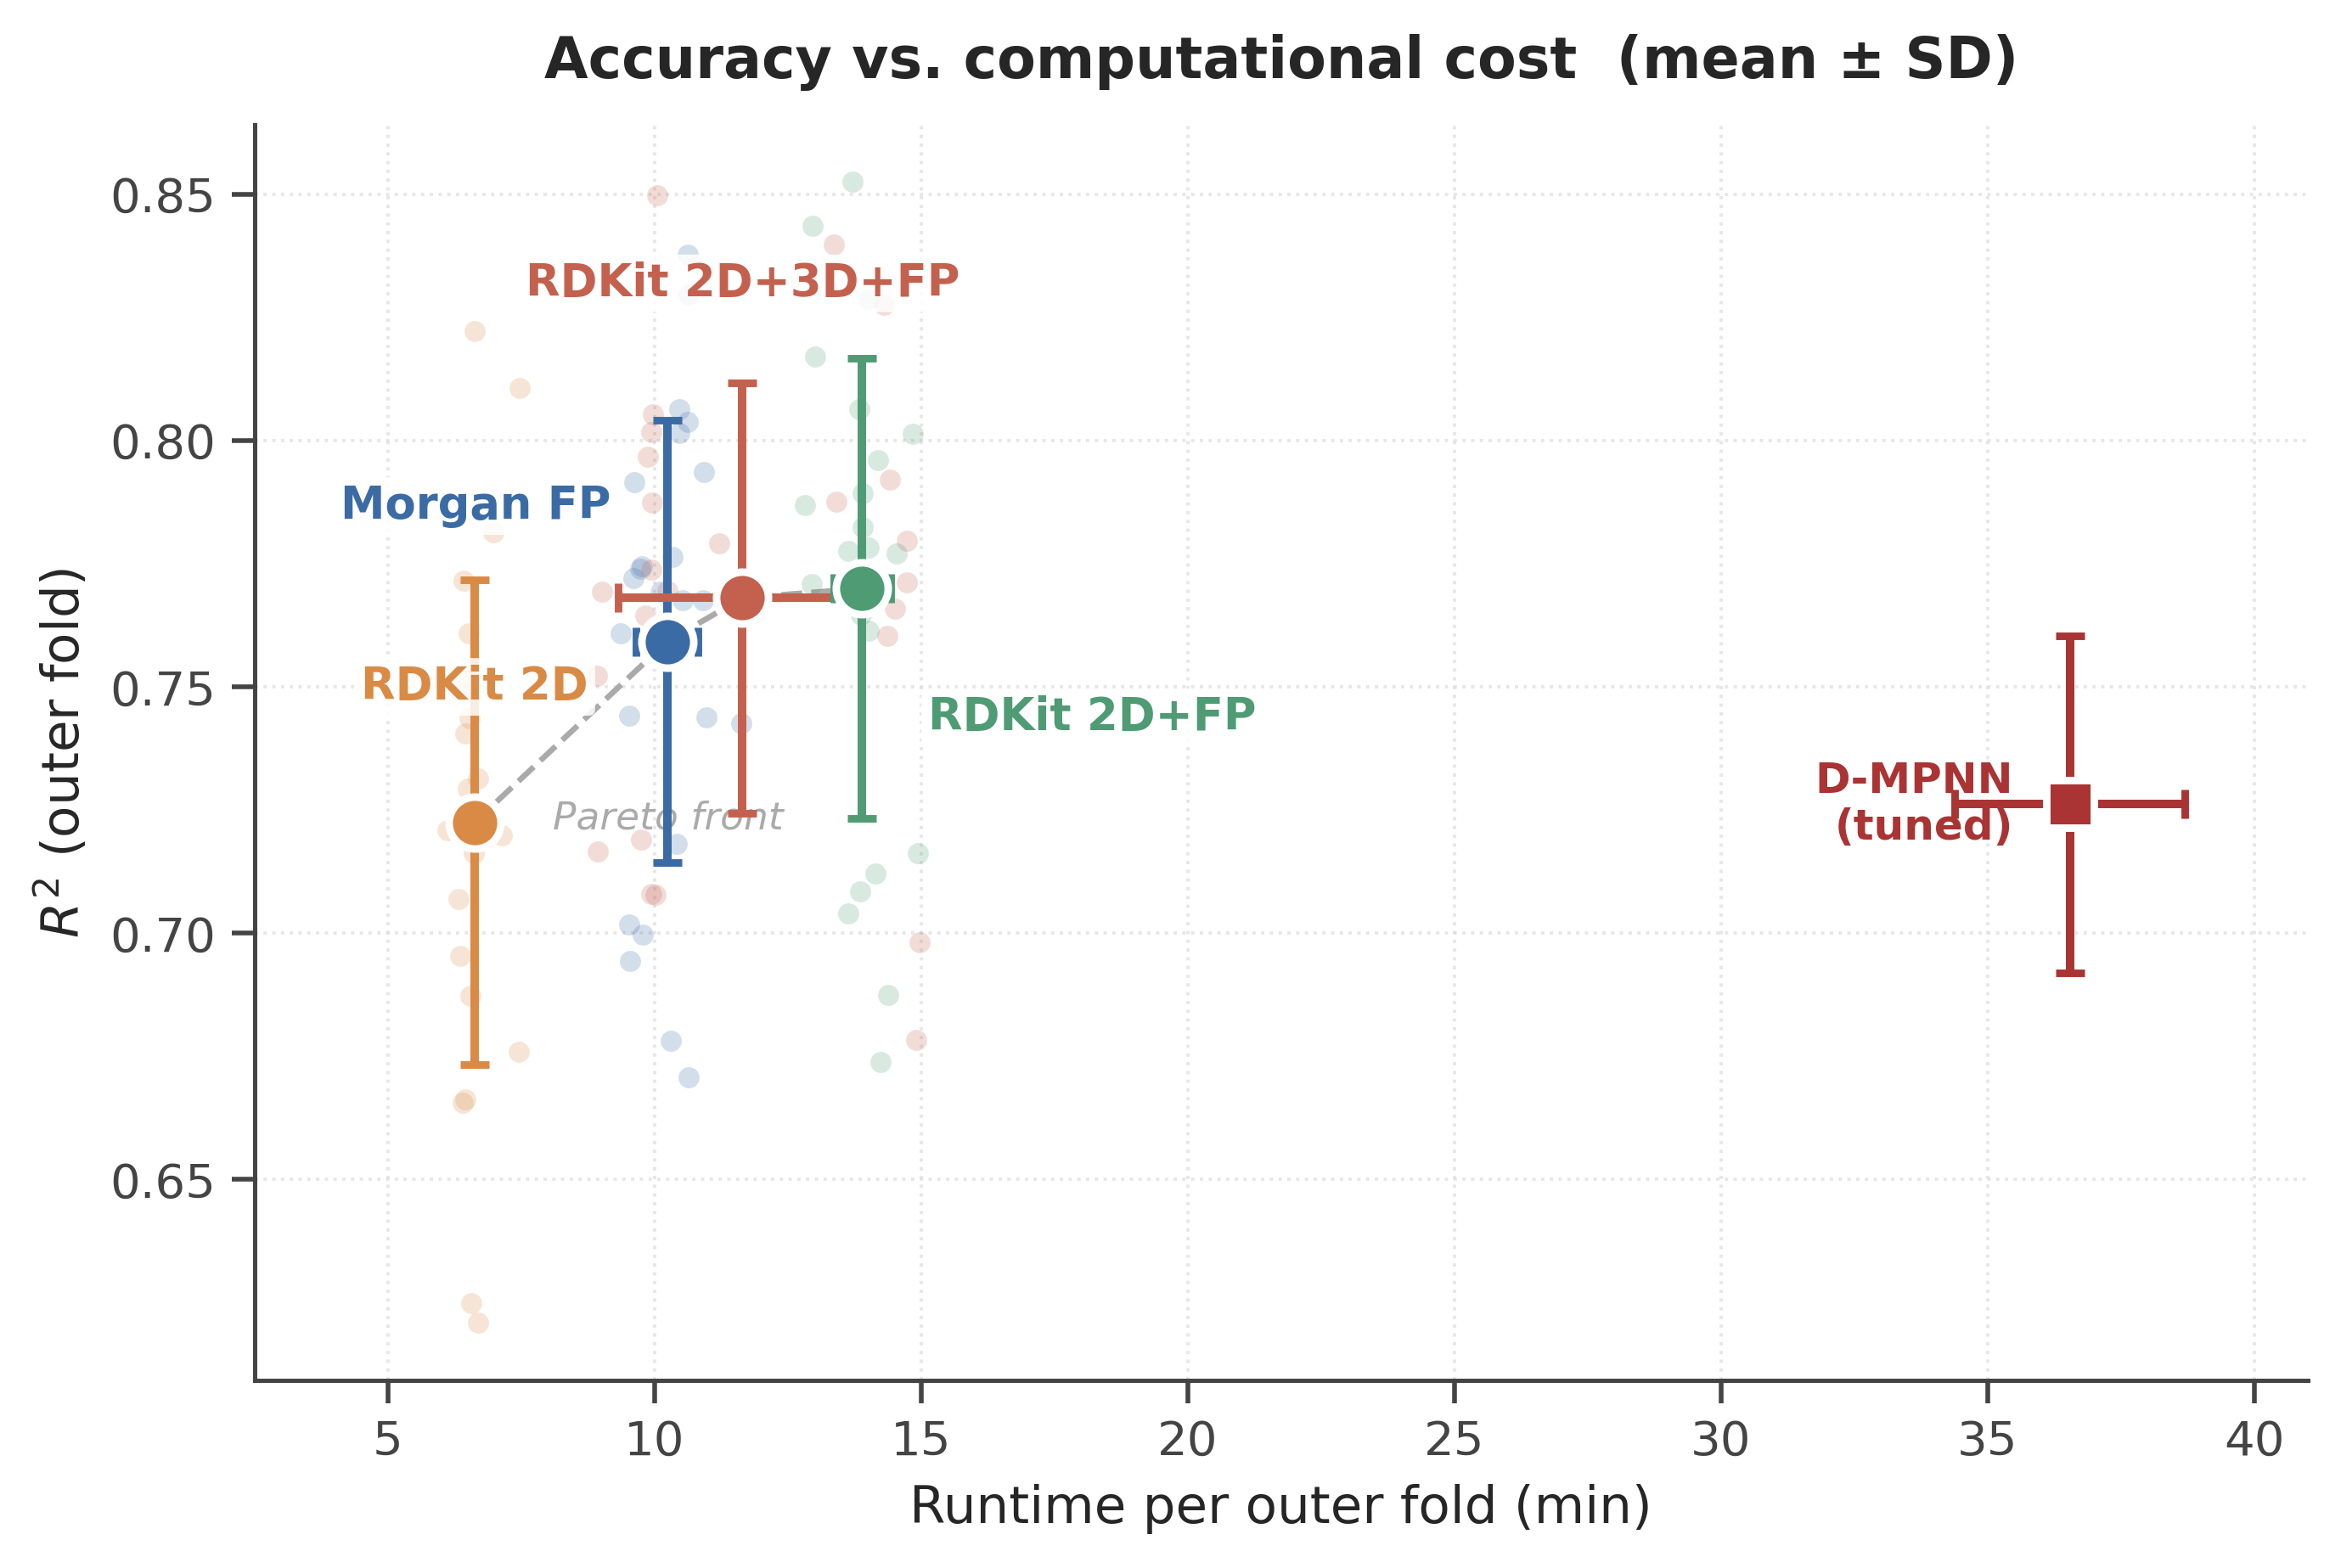
\includegraphics[width=0.85\textwidth]{figures/01_nested_cv_time_vs_performance.png}
	\caption{Accuracy versus run time per outer fold (mean $\pm$ SD over the \TotalOuterFolds\ folds; faint dots are individual folds). Only models that include a model-selection step are shown: the classical ensembles with their inner architecture search and the D-MPNN with a nested search over \GnnTunedNConfigs\ configurations; the default D-MPNN, which has none, is reported in Table~\ref{tab:cost}. Times are not normalized by thread count.}
	\label{fig:cost_accuracy}
\end{figure}

The parsimonious choice for this target is therefore the 2D fingerprint ensemble. This is a statement about information content and about the inputs the screening step needs, not a measured speed advantage; as shown in Section~\ref{sec:gnn_results}, the end-to-end benchmark of the classical protocol was not faster than the graph network.

% ==========================================
% 4. SECTION 4.3
% ==========================================

\subsection{Methodological Scope, Limitations, and Translational Potential}

The reliability of any quantitative structure--activity relationship (QSAR) model is bounded by the chemical diversity of its training data. With \NCompounds\ compounds, the applicability domain of the ensemble is restricted to the scaffolds and physicochemical ranges of the curated TgDHFR set, and the FDA drugs are far from it: their median similarity to the five nearest training compounds is \ScreenADFdaMedian, against \ScreenADTrainMedian\ for the training compounds among themselves, so most predicted potencies in the screening are extrapolations that the applicability domain cannot vouch for. The cross-validation estimate also needs a caveat: the main folds were random, and scaffold-grouped splits (Section~\ref{sec:scaffold_results}) lowered $R^2$ by about 0.2 for both the Morgan ensemble (from $\RandomMorganRTwoMean$ to $\ScaffoldMorganRTwoMean$) and the D-MPNN (from $\RandomGnnRTwoMean$ to $\ScaffoldGnnRTwoMean$). The reported $R^2$ therefore describes interpolation among related compounds, and the expected accuracy on the structurally distant drugs of the FDA library is closer to the scaffold-split values. We did not evaluate temporal splits. The predicted potencies of those drugs have no experimental counterpart in this study.

Activity cliffs are a specific weakness of 2D circular fingerprints in this setting: very similar molecules can differ strongly in activity, and a Morgan bit vector may map them to nearly the same representation. We did not measure how many cliffs the data set contains or how the model behaves on them. The docking step does not remove the problem either; it adds an independent estimate, but a rigid-receptor Vina score is itself unreliable for small differences between close analogs, as the discordance for pyrimethamine in Section~\ref{sec:consensus_results} illustrates.

The inner architecture search is a further source of instability. Evaluating \NArchitectureCombos\ stacking combinations per outer fold carries a risk of selection bias. The nested design keeps this search away from the outer test folds, so the estimate is not inflated by it, but the chosen architecture varied across folds: within the Morgan space, \MorganBestArchitecture\ was the most frequent choice yet was selected in only \MorganStability\% of the \TotalOuterFolds\ folds (Figure~S1 of the Supplementary Material). With a data set of this size the inner loop does not converge on a single architecture, and the reported performance should be read as that of the selection procedure and not of one fixed ensemble.

The ADMET step (Section~\ref{sec:admet_results}) shows how much the final list depends on the filters: triamterene, the most efficient candidate of the ML screen, was removed on a predicted hERG probability of \AdmetHergTriamterene{} from a Random Forest trained on \AdmetNHergTrain\ compounds whose accuracy we did not evaluate, so the flag is a reason to test the compound and not a reason to discard it. The parenteral label given to pralatrexate and methotrexate comes from a passive-permeability model and should not be read as a statement about clinical use: methotrexate, for example, is also given orally, because its absorption is carrier-mediated and is not captured by a passive-permeability predictor.

The most important translational limitation is selectivity. Pralatrexate, methotrexate and trimetrexate are anticancer antifolates that inhibit human dihydrofolate reductase, and are cytotoxic to host cells. Our pipeline predicts potency against the parasite enzyme and ranks docking energies against it, but it does not assess selectivity over the human enzyme, so a high rank should not be mistaken for a therapeutic candidate. The consensus hits are best read as computational hypotheses: compounds whose predicted activity is supported by two independent methods and that merit selectivity docking against human DHFR and experimental testing. The same pipeline could be applied to other targets with small data sets, but our results do not show that it transfers; that would need to be tested on those targets.

\subsection{Conclusions and Future Directions}

This study compared classical machine learning ensembles with a graph neural network on a small TgDHFR data set ($N = \NCompounds$), under a leakage-free nested cross-validation protocol, and applied the best classical model to a library of FDA-approved drugs with an orthogonal docking check. Three conclusions follow.

First, on this data set a classical stacking ensemble on 2D Morgan fingerprints performed at least as well as the alternatives we tested. It reached $R^2 = \MorganRTwoMean \pm \MorganRTwoStd$, against $\ChemPropDMPNNFoldRTwoMean \pm \ChemPropDMPNNFoldRTwoStd$ for a default D-MPNN and $\GnnTunedRTwoMean \pm \GnnTunedRTwoStd$ for one tuned in a nested search; the difference ($\Delta R^2 = \GnnTunedVsMorganDiffRTwo$ for the tuned network) was small but survived multiple-comparison correction, and equivalence with the Morgan ensemble could not be established in either metric, so the network as usually trained is behind the fingerprint-based ensembles rather than interchangeable with them. The gap is one of training budget and not of architecture: averaging five networks narrows it, and a D-MPNN initialized from a pretrained model reaches $\ChemeleonRTwoMean$ and is the only model equivalent to the Morgan ensemble in both metrics, at \ChemeleonCostFactor\ times the computational cost and without exceeding it. Adding 3D descriptors to the fingerprint-based sets changed nothing detectable. Feature selection and Gaussian-noise augmentation, which the original study credited with large gains, did not improve a classical learner under the same hold-out protocol. Those gains are accounted for by information leaks: removing them one at a time from the published code takes its $R^2$ from \KarLadderRungZeroRTwoMean\ to \KarLadderRungFourRTwoMean, and the same selection applied leakily to a classical learner reproduces them (\ExpBleakyRTwoMean\ against \ExpBRTwoMean). These findings are limited to a single target and a comparison in which the network search was modest; they do not show that graph networks cannot match fixed fingerprints. The classical protocol was also not cheaper to run: the benchmark took longer than the network's, and its advantage lies in accuracy that is not lower, simpler inputs, and a deployed model that needs only a subset of fingerprint bits.

Second, nested cross-validation and a careful curation of the data (removal of duplicates and of two extreme potency values, with a sensitivity analysis of the latter) were necessary to obtain estimates that can be compared across models. Our random-split estimates are also optimistic: with scaffold-grouped splits every model lost between \ScaffoldChemeleonDropRTwo\ and \ScaffoldRdkitTwoDDropRTwo\ units of $R^2$ (to $\ScaffoldMorganRTwoMean$ for the Morgan ensemble and $\ScaffoldGnnRTwoMean$ for the D-MPNN), and the data could not resolve the differences between them. The loss was smallest for the pretrained network, so what representation learning offers on this data set is robustness to a change of chemotype rather than accuracy within one.

Third, combining ML prediction with docking produced a short, reproducible list of hypotheses and not validated leads. Only \ScreenNDomain{} of the \ScreenNStructural{} scored compounds fell inside the model's applicability domain, the agreement between predicted potency and docking energy was weak ($\rho = \DockSpearmanRho$, $p = \DockSpearmanP$), and the compounds leading the ranking by potency are antifolates that also inhibit the human enzyme, whose selectivity was not assessed.

Future work should therefore (i) dock the consensus hits against human DHFR and test them in enzymatic assays against TgDHFR, (ii) evaluate temporal splits, (iii) compare against larger searches and pretrained graph models, and (iv) apply the pipeline to other targets before claiming that it generalizes.



	% The declarations publishers ask for, in the order they are most often requested. Each one is a file of its own so
% that a statement is written once and every layout reports the same thing; the heading, and whether the set is
% gathered under one of its own, is the layout's business, which is what \projdeclaration supplies. Adding a
% journal means defining that command and reordering these lines, not rewriting the statements.
\projdeclaration{Availability of data and materials}{sections/06_1_Data_Available.tex}
\projdeclaration{Competing interests}{sections/06_2_Competing_Interests.tex}
\projdeclaration{Funding}{sections/06_3_Funding.tex}
\projdeclaration{Authors' contributions}{sections/06_4_Authors_Contributions.tex}
\projdeclaration{Acknowledgements}{sections/06_5_Acknowledgements.tex}
\projdeclaration{Declaration of generative AI use}{sections/06_6_Generative_AI.tex}

	
	% \printcredits is left out on purpose: the contributions are declared once, in
	% sections/06_4_Authors_Contributions.tex, so that every layout reports the same thing. The
	% \credit entries above stay for the journal's own metadata.
	
	%% Loading bibliography style file
	%\bibliographystyle{model1-num-names}
	\bibliographystyle{cas-model2-names}
	
	% Loading bibliography database
	\bibliography{references_nourl.bib}
	
	% Biography
	%\bio{}
	% Here goes the biography details.
	%\endbio
	
	%\bio{pic1}
	% Here goes the biography details.
	%\endbio
	
\end{document}

